\setcounter{chapter}{11}
\chapter{第一原理计算}\label{chap:quantum-calculation}
\section{密度泛函理论基础} \label{section:dft}

二十世纪二十年代,Thomas-Fermi{建议的自由电子模型}\cite{PCPS23-542_1927,ZP48-73_1928}中,将经典体系的总能表示成为电子密度$\rho$的函数\cite{Parr-Yang,CR91-651_1991},可以看成密度泛函(Density Functional)思想的源头;五十年代Slater用局域电荷密度代替离域的波函数乘积,该近似简化了Hartree-Fock方法\cite{MPCPS24-111_1928,ZP61-126_1930, PR32-339_1928}交换能的计算,这就是著名的X\,$\alpha$方法\cite{PR81-385_1951}。该方法表明,考虑量子效应后的电子体系,能量可以用电子密度近似表示
。%这些研究都显示,体系的能量有可能表示成为基态密度的函数。 %最早}) {思想的源头}可以上溯到%理论})
相比于波函数,用电子密度表示体系总能量,最大的优点是有效地减少变量的数目,%方便了应用理论方法研究电子体系,
X\,$\alpha$方法带动了采用密度泛函表示体系性质的可行研究的深入。但是真正将
密度泛函理论\textrm{(Density Functional Theory,~DFT)}确立为严格的理论,要等到六十年代,Hohenberg和Kohn%最基本的变量是体系单粒子})
完成密度泛函理论的基本定理的证明\cite{PR136-B864_1964}。
Hohenberg-Kohn定理表明,体系的基态性质(如总能量)完全由%单})
%粒})
基态{电}子密度决定;随后,Kohn和Sham\cite{PR140-A1133_1965}%采用了与相互作用体系有相同单粒子密度的无相互作用体系的动能近似来近似计算相互作用体系的动能,把剩余部分都放在交换-相关能项中予以考虑。本质上,这个方法把单粒子波函数又引入了密度泛函理论,但是基本解决了动能计算的问题。在他们的工作基础上,各种近似的交换-相关能泛函形式\cite{CJP58-1200_1980,PRB45-13244_1992,PRA38-3098_1988,PRB33-8822_1986,PRB37-785_1988}被提出来并})
{提出了用基态密度表示体系总能量的成近似方案,使密度泛函理论可应用于实际体系的量子力学计算。七十年代之后,密度泛函理论的研究主要集中在寻求更精确的能量密度泛函表达形式上,其中有些泛函已被}广泛应用于%计算各类})
原子、分子和固体体系{的计算中\cite{CJP58-1200_1980,PRB45-13244_1992,PRA38-3098_1988,PRB33-8822_1986,PRB37-785_1988}}。

\subsection{Hohenberg-Kohn定理}
Hohenberg-Kohn定理\cite{PR136-B864_1964}包含两部分{内容}:
\begin{itemize}
	\item 第一部分指出,多%粒})
{电}子体系的外势由其%基态性质与
基态%单})
%粒})
{电}子密度%之间存在一一对应关系,这部分是密度泛函理论的基础
决定(除可能相差一个常数以外),从而体系的基态波函数以及所有其它性质均由其基态电子密度决定
;\item 第二部分指出体系基态总能量{泛函}在体系基态%单})
%粒})
{电}子密度处取极小{值},这部分%给出})
{提供}了从%单}) %粒})
{电}子密度计算体系基态能量的基本方法。
\end{itemize}
%Hohenberg-Kohn
简单证明如下:

%设})
N个粒子相互作用量子力学体系的%Hamiltonian})
{基态总能量}可表示为:
\begin{equation}
	{E_{\mathrm{gs}}[\Psi]}%F_{\mathrm{HK}}[\rho]})
=\langle\Psi%[\rho]})
|\hat{T}+\hat{V}+\hat{W}|\Psi%[\rho]})
\rangle
	\label{eq:DFT_01}
\end{equation}
其中$\hat{T}$是动能算符,$\hat{V}$是外势%、即通常的局域单粒子势})
,$\hat{W}$为%粒})
{电}子间相互作用势{,$|\Psi\rangle$是基态波函数}。假设两个体系的外势分别为$\hat{V}$和$\hat V^{\prime}$,它们之间相差不为常数,这两个体系的非简并基态分别为$|\Psi\rangle$和$|\Psi^{\prime}\rangle$,其基态的本征方程分别为:
$${\hat H\Psi=}\bigl(\hat{T}+\hat{V}+\hat{W}\bigr)|\Psi\rangle=E_{\mathrm{gs}}|\Psi\rangle$$
$${\hat H^{\prime}\Psi=}\bigl(\hat{T}+\hat V^{\prime}+\hat{W}\bigr)|\Psi^{\prime}\rangle=E_{\mathrm{gs}^{\prime}}|\Psi^{\prime}\rangle$$

%假设})
{根据量子力学原理,}$|\Psi\rangle{\neq}|\Psi^{\prime}\rangle$,%则上两式相减可得}):
% $$%\big(\hat{V}-\hat V^{\prime}\big)|\Psi\rangle=\big(E_{gs}-E^{\prime}_{gs}\big)|\Psi\rangle}) $$
%因为$\hat{V}$和$\hat V^{\prime}$是乘积算符,从上式可知,$\big(\hat{V}-\hat V^{\prime}\big)=\big(E_{gs}-E^{\prime}_{gs}\big)=\text{const}$,这与$\hat{V}$和$\hat V^{\prime}$之间相差不为常数矛盾,因此$\hat{V}$和$|\Psi\rangle$之间存在一一对应关系。})
由变分原理可知:
$$E_{\mathrm{gs}}=\langle\Psi|\hat{H}|\Psi\rangle<\langle\Psi^{\prime}|\hat{H}|\Psi^{\prime}\rangle$$

设$|\Psi\rangle$和$|\Psi^{\prime}\rangle$对应的%单})
%粒})
{电}子密度分别为$\rho(\vec{r})
$和$\rho^{\prime}(\vec{r})$,{$v(\vec r)$为单个电子受到的外势的作用能,则}有
$$\langle\Psi^{\prime}|\hat{H}|\Psi^{\prime}\rangle=\langle\Psi^{\prime}|\hat H^{\prime}+\hat{V}-\hat V^{\prime}|\Psi^{\prime}\rangle=E^{\prime}_{gs}+\int{\rho^{\prime}(\vec{r})[v(\vec{r})-v^{\prime}(\vec{r})]\textrm{d}^3\vec{r}}$$
%相应的,从$E^{^{\prime}}_{gs}$出发})
{类似地}可以得到不等式
$$E^{^{\prime}}_{gs}<E_{gs}+\int{\rho(\vec{r})[v^{\prime}(\vec{r})-v(\vec{r})]\textrm{d}^{3}\vec{r}}$$

%假设})
{如果}$\rho(\vec{r})\!=\!\rho^{\prime}(\vec{r})$,把上面两个不等式相加可以得到$E_{gs}+E^{\prime}_{gs}\!<\!E_{gs}+E^{\prime}_{gs}$,这显然%与假设矛盾,因此$\rho(\vec{r})$与v可以表示的基态$|\Psi\rangle$之间有一一对应关系})
{不能成立。亦即不可能出现不同的外势产生相同的电子密度的情况}。由此可以得出结论,体系的基态%单})
%粒})
{电}子密度和体系的外势(除了相差一个常数之外)一一对应%,})
{。}%也就是说,})
{因为$\rho(\vec r)$唯一地确定体系中电子的数目$N$,故}体系%的一切})
{%基态
的\textrm{Hamiltonian}、从而全部}性质都%可以})
由体系的基态%单})
%粒})
{电}子密度完全决定。{特殊地,体系基态总能量是它的基态电子密度的泛函,记作$E[\rho]$。
	
设有一电子密度$\tilde\rho(\vec r)$,满足约束条件
\begin{displaymath}
	\begin{aligned}
		\tilde\rho(\vec r)\!&\geqslant\!0\\
		\int\tilde\rho(\vec r)\textrm{d}^3\vec r&\!=\!N
	\end{aligned}
\end{displaymath}
$\tilde\rho(\vec r)$来自某个\textit{v}\,-\,可表示的基态波函数$\tilde\Psi$(称为\textit{v}\,-\,可表示的电子密度)。设与体系基态波函数$\Psi$对应的电子密度为$\rho_0(\vec r)$,若$\tilde\rho(\vec r)\!\neq\!\rho_0(\vec r)$,则根据上面的讨论可知,$\tilde\Psi\!\neq\!\Psi$,$E[\tilde\rho]$\,$\geqslant$\,$E[\rho_0]$。}

%从上面的结论我们可以定义作为单粒子密度$\rho(\vec{r}) $泛函的体系基态能量的形式。设一$N$个粒子体系的外势场为$\hat{V_{0}}$,})
{设}与$\rho(\vec{r})$%一一})
对应的%某一N个粒子})
体系波函数为$|\Psi[\rho]\rangle$,%定义该})
体系的基态总能量作为$\rho(\vec{r})
$的泛函%形式})
{可表达}为:
\begin{equation}
	E[\rho]=\langle\Psi[\rho]|\hat{T}+\hat{V}+\hat{W}|\Psi[\rho]\rangle
	\label{eq:DFT_02}
\end{equation}
%由变分原理可知,体系本身的基态单粒子密度使得$E_{v_{0}}[\rho]$取极小,因此可以通过寻找能量泛函的极小值点来确定体系的基态能量和基态粒子密度}
{因为由外势产生的势能是电子密度$\rho(\vec r)$的简单泛函,}体系的{基态}总能量泛函可以写成:
\begin{equation}
	E[\rho]=F_{\mathrm{HK}}[\rho]+\int\rho(\vec{r})v(\vec{r})\textrm{d}^3\vec{r}
	\label{eq:DFT_03}
\end{equation}
其中$F_{\mathrm{HK}}[\rho]=\underset{\Psi\to\rho}{\mathrm{Min}}\langle\Psi[\rho]|\hat{T}+\hat{W}|\Psi[\rho]\rangle$%。})
{,}%从上式可以看出,$F_{\mathrm{HK}}$的形式}
与%$v_{0}$})
{$v(\vec r)$}没有关系,%只与动能和离子间相互作用能的形式有关。对于我们最通常研究的原子、分子和固体体系而言,$F_{\mathrm{HK}}$的形式都是一致的。但是})
{是一个普适的能量泛函。}

到目前为止,$F_{\mathrm{HK}}$的%具体})
{精确表达形}
式还没有得到,%一般都采用近似的方法})
{只能作近似处理}。Thosmas-Fermi%理论})
{模型}%实际上就是一个对$F_{\mathrm{HK}}$近似的理论,但是由于动能泛函的误差很})
{可以看作是对$F_{\mathrm{HK}}[\rho]$泛函采取粗略近似的密度泛函理论。由于误差太}大,Thomas-Fermi%理论})
{模型}既不能%得到})
{说明}原子体系%正确的})
电子密度的壳层结构,也不能%得到})
{说明存在}稳定%的})
分子{的事实}。%后来经过})
Dirac\cite{PCPS26-376_1930}和Weizsacker\cite{ZP96-431_1935}对能量泛函的改进取得%了})
一定%的进展})
{成功},但%是同实验结果相比,仍然有比较大的差距})
{没有取得实质性的进展}。

\subsection{Kohn-Sham方程}
%对于})
{根据}Hohenberg-Kohn定理,只要%得到})
{知道}体系的总能量的{密度}泛函形式,就可以通过对%单})
%粒})
{电}子密度%作})
变分求得体系的基态%单粒})
{总能量和基态的电}子密度%和基态能量})
。与%通常的})
对波函数%作})
变分求%得})
体系基态%性质})
{总能量}的方法相比,波函数是3N%-维})
{维空间中的}函数,而%单})
%粒})
{电}子密度只是三维{空间中的}函数,因此这种方法有%巨})
{很}大的优越性。但是%由于很难})
{迄今无法}得到%比较})
精确的能量密度
泛函形式,特别是体系的动能密度
泛函的精确%度对计算体系性质有很大的影响})
{形式。为避开这一困难},Kohn和Sham\cite{PR140-A1133_1965}提出%了用具有与相互作用体系单粒电子密度相同但无相互作用体系的动能来近似计算相互作用体系动能的方法,这种})
{以下}方法%比较好地})
解决%了})
动能泛函的计算问题。%他们的})
具体%计算})
方法如下:假设存在一个外势为$v_s$的无相互作用多%粒})
{电}子体系,其基态%单})
%粒})
{电}子密度$\rho$与%我们所})
{要}研究的一个多电子相互作用体系的基态%单})
%粒})
{电}子密度相同。这个无相互作用体系的%单})
%粒})
{电}子密度为:
$$\rho(\vec{r})=\sum_{i=1}^{N}\langle\varphi_{i}|\vec{r}\rangle\langle\vec{r}|\varphi_{i}\rangle$$
其中$\varphi_i(i\!=\!1,\cdots,N)$是该体系能量最低的$N$个{单电子}本征态。该体系的动能为:\linebreak $T_{s}[\rho]\!=\!\sum\limits_{i=1}^{N}\langle\varphi_{i}|\hat{T}|\varphi_{i}\rangle$。
用这个无相互作用体系的动能作为%我们})
{要}研究的相互作用体系的动能近似{值},可以把相互作用体系的%动能})
{基态能量密度泛函}写成如下形式:
\begin{equation}
  \label{eq:dft-1}
E[\rho]=T_{s}[\rho]+\int{v(\vec{r})\rho(\vec{r})\textrm{d}^3\vec{r}}+\frac 12\iint{\rho(\vec{r})w(\vec{r},\vec r\,^{\prime})\rho(\vec r\,^{\prime})\textrm{d}^3\vec{r}\textrm{d}^3\vec r\,^{\prime}}+E_{XC}[\rho]
\end{equation}
其中{$w(\vec r, \vec r\,^{\prime})$为两个电子间的相互作用能。}交换-相关能泛函的形式为:
\begin{equation} 
  \label{eq:dft-2}
  E_{XC}[\rho]=F_{\mathrm{HK}}[\rho]-\frac 12\iint{\rho(\vec{r}) w(\vec{r},\vec r\,^{\prime})\rho(\vec r\,^{\prime})\textrm{d}^3\vec{r}\textrm{d}^3\vec r\,^{\prime}}-T_{s}[\rho]
\end{equation}
利用$T_s$和$\rho$的表达式,%对})
{由}总能量%作})
{在$\{\varphi_i, i\!=\!1,\cdots, N\}$满足正交归一条件下对$\{\varphi_i\}$}变分,即%可以})
得到Kohn-Sham方程:
\begin{equation} \label{eq:dft-3}
	\bigl(\hat{T}+\hat{V}_{\mathrm{eff}}\bigr)|\varphi_{i}\rangle=\varepsilon_{i}|\varphi_{i}\rangle{,\quad i=1,\cdots,N,\cdots}
\end{equation}
其中
\begin{equation} \label{eq:dft-4}
	V_{\mathrm{eff}}(\vec{r})={v}(\vec{r})+\int{w(\vec{r},\vec r\,^{\prime})\rho(\vec r\,^{\prime})\textrm{d}^3{\vec r\,^{\prime}}+\frac{\delta E_{XC}}{\delta\rho(\vec{r})
}}
\end{equation}
式\eqref{eq:dft-4}右边第一项%中})
${v}(\vec{r})
$为外势,第二项为%粒})
{电}子间经典的{Coulomb}相互作用势,第三项是交换-相关势。%对于我们所关心的原子、分子和固体等多电子体系而言,\eqref{eq:dft-4}式中的外势为核吸引势,粒子间经典相互作用势是电子间的Coulomb势。})

以上推导中假设任意一个相互作用%的{\it v}-可表示的单粒})
{体系的基态电}子密度%也是})
{都有一个}与之有相同基态电子密度的无相互作用%的{\it v}-可表示单粒})
{的体系相对应}。可以证明,按照该方法构造的无相互作用体系基态如果是非简并的,即这个无相互作用体系的基态可以用单行列式波函数表示,则用这个单行列式波函数构造的%单粒})
{基态电}子密度与相互作用体系的%单粒})
{基态电}子密度是一致的%,但是如果无相互作用体系的基态是简并的,相互作用{\it v}-可表示单粒子密度是否仍然与由单行列式波函数构造的无相互作用体系单粒子密度对应的问题还没有得到解决})
。\cite{PNAS76-6062_1979,IJQC24-243_1983}

对于{电子}自旋{密度}%极化的情况,从})
{不恒为零的体系,推广}Hohenberg-Kohn定理%可以知道,体系基态自旋为})
{的推导过程和近似处理方法,可以得到对于体系的}$\alpha$%})
自旋和%为$\beta$的})
{$\beta$自旋}电子的{\textrm{Kohn-Sham}方程,被称为自旋密度泛函理论\textrm{(SDFT)}。}%密度从原理上可以由体系总电子密度完全决定;但是如果要研究})
{在}研究一些体系的磁学性质或者处于解离极限的分子的性质{时},%在现有泛函基础上,只有})
采用%把自旋$\alpha$和自旋$\beta$的电子分开处理的})
自旋密度泛函方法才能得到合理的结果{。}%而且})
对于开壳层体系%而言})
,用自旋密度泛函方法%的结果})
通常比不{区}分自旋的密度泛函方法结果要好。%自旋密度泛函理论的基本原理和Kohn-Sham方程很容易用类似的推导方法得到,在此不作推导了。})

Kohn-Sham方程的%这个})
实质,是把动能泛函的主要部分分离出来,将剩余%不太重要的动能})
部分放到交换-相关能中。由于该方程%基本})
{比较好地}解决了%计算})
动能泛函的{计算}问题,%这个方法})
使得密度泛函方法能够比较精确地研究电子体系的性质。有必要指出,Kohn-Sham方程虽然把单%粒})
%{\kaishu 电}
电子波函数引进密度泛函理论,但它是{\heiti 形式上的单粒子方程},%从理论上讲只利用单Slater行列式就})
因为方程中包括泛函的形式表示的交换-相关作用%计算})
,这是对电子间的多体关联的一种近似考虑,%而传统的量子化学方法如果要考虑电子之间的相关能效应,则必须采用多Slater行列式的方法,Kohn-Sham方程})
{相比}传统的量子%化})
{力}学方法,密度泛函方法有明显的%})
优越%性})
{之处},基于Kohn-Sham方程的密度泛函方法也成为电子尺度计算最重要的{理论}方法之一。

\subsection{交换-相关能泛函}
Kohn-Sham方程%从})
理论上%讲})
是%一个})
严格的方程,但是要把它用于具体计算,就需要%解决})
{知道}交换-相关能泛函的具体形式。%从上一节的推导可以看出,})
Kohn-Sham%理论})
提出的交换-相关能的含义与从头计算方法的交换和相关能的含义有%很})
{较}大的差别{。现有}密度泛函理论中,习惯上将交换能定义为用Kohn-Sham轨道按照Hartree-Fock交换能%形})
{表达}式计算得到的能量,相关能则包含两部分,一部分是相互作用体系动能和对应的无相互作用体系动能{之}差,另一部分是相互作用体系中粒子间的相互作用能与经典相互作用{能}和交换能%的})
{之}差。密度泛函{理论}中的交换-相关能泛函的精确形式还%没有})
{无法}得到,只能通过{考虑}一些{应满足的}具体%的})
物理%考虑})
{条件}和合理的假设得到近似的交换-相关能泛函。最简单的近似就是由Kohn和Sham提出的局域密度近似%方法})
{泛函}(local density approxmiation, LDA)\cite{PR140-A1133_1965}{。}交换-相关能{泛函}的具体形式取为:
\begin{equation}
  \label{eq:dft-5}
  E_{XC}^{\mathrm{LDA}}[\rho]=E_X^{\mathrm{LDA}}[\rho]+E_C^{\mathrm{LDA}}[\rho]=\int\varepsilon_X[\rho]\rho(\vec{r}) \textrm{d}^3\vec{r}+\int\varepsilon_C[\rho]\rho(\vec{r}) \textrm{d}^3\vec{r}
\end{equation}
其中$\varepsilon_X[\rho]$和$\varepsilon_C[\rho]$分别为{一个电子的}交换能和相关能%密度})
。上式表明空间每一个点的交换能密度和相关能密度只是取决于该点的电子密度,而与其他点的电子密度无关。对{于均匀电子气,}$\varepsilon_X[\rho]$和$\varepsilon_C[\rho]$%的选取可按照均匀电子气中交换-相关能和电子密度的关系得到,})
{为常数%,等于体系的总电子交换能(或相关能)除以体系的体积和电子密度
。}对于非均匀电子气%而言})
,%这样选取的$e_X(\rho)$和$e_C(\rho)$的物理图象相当于})
{可以设想}把空间分割为无穷多个%非常})
{无限}小的区域,%假设})
{可以认为}电子的密度在每个小的区域内都是均匀的,每个小区域中的交换-相关能都%采用})
{可以按}均匀电子气%模型下})
的交换-相关能{计算},整个体系的交换-相关能就可以写成\eqref{eq:dft-5}式的形式。局域密度近似基于均匀电子气模型得到的,直觉上,应该主要对于电子密度变化缓慢的体系{才会}是%个})
比较好的近似,而实际上对于原子、分子和某些价电子密度%变化})
剧烈变化的固体,局域密度近似方法仍然能够得到比较合理的结果。不过,为了进一步提高密度泛函方法对原子、分子以及扩展体系的计算精度,应该需要考虑%到})
电子密度的不均匀性。通过引入电子密度的梯度对{局域近似的}交换-相关能的{泛函}形式加以校正,%即所谓的})
{就是}梯度展开近似(Gradient Expansion Approximation, GEA)%和})
{或}一般梯度近似(Generalized Gradient Approximation, GGA),%即})
此时能量泛函不仅依赖于局域密度值的分布,还与密度梯度有关,这在一定程度上改善LDA的计算结果。比较重要的GGA交换能泛函有P86$_x$\cite{PRB33-8800_1986}、B88\cite{PRA38-3098_1988}、PW91\cite{PRB46-6671_1992,PRB48-4978_1993,PRB54-16533_1996,PRB57-14999_1998}、PBE\cite{PRL77-1396_1996,IBID78-1396_1997}、HCTH\cite{JCP109-6264_1998}等。

由于在交换-相关能泛函的定义中包含了一部分动能的贡献,因此很多研究者考虑{到}在交换-相关{能}泛函中应该包括动能密度为变量,%这就是所谓的})
{提出}\textit{meta}-GGA泛函。自1980年代末以来,比较有代表性的\textit{meta}-GGA交换能泛函有BR89\cite{PRA39-3761_1989}、\linebreak VSXC\cite{JCP109-400_1998}、tauPBE\cite{JCP111-911_1999}、PKZB\cite{PRL82-2544_1999,PRL82-5179_1999}、B00\cite{JCP112-4020_2000}、PCS00\cite{JCP113-10013_2000}等。

为了提高各种近似{能量}泛函的%计算结果的})
精度,从1990年代初起,基于绝热关联\textrm{(adiabatic connection)}%(下面会详述)})
{的推理},Becke提出把部分按Hartree-Fock方法计算的交换能加入到能量密度泛函中的思想{,}%从而})
构造出了一系列%的所谓})
杂化型%的})
交换-相关{能}泛函,其中比较重要的是“半对半(half and half)”泛函\cite{JCP98-1372_1993}、B3P\cite{JCP98-5648_1993}、B3LYP\cite{JPC98-11623_1994}、B1B95\cite{JCP104-1040_1995}等。

由于%对})
相关能的物理%定})
{含}义不%很})
{够}清晰,而且相关能的数值比交换能小一个数量级,既比较难准确估计,又不是计算中误差的最主要来源,因此提出的{近似}相关能泛函%模型})
比交换能泛函%模型})
少一些。最早提出把相关能表示成电子密度泛函的是Wigner\cite{PR46-1002_1934},他的公式适用于均匀电子气:
\begin{equation}
  E_C=-\dfrac a{r_s+b}
  \label{eq:dft-16}
\end{equation}
其中$a$、$b$是参数,$r_s$\,=\,$\left(\dfrac3{4\pi\rho}\right)^{\frac13}$称为表观半径。%实际上})
对%于})
均匀电子气的相关能并没有统一\linebreak 的解析式。von Barth\cite{JPC5-1629_1972}和Gunnarsson\cite{PRB13-4274_1976}等人都提出过一些近似的式子。1980年,\linebreak Vosko、Wilk和Nusair\cite{CJP58-1200_1980}利用Ceperley和Alder\cite{PRL45-566_1980}用量子Monte Carlo方法计算得到的{均匀电子气}相关能数据拟合出一个%均匀电子气的})
相关能的%公})
{表达}式,即最常用的VWN%公})
{表达}式。后来Perdew和Wang\cite{PRB45-13244_1992}把他们的%公})
{表达}式简化并重新拟合了参数。

以上相关能%公式})
{泛函}都是针对均匀电子气的,比较常用的考虑了梯度校正的相关能泛函%公})
{表达}式有P86$_c$\cite{PRB33-8822_1986}、LYP\cite{PRB37-785_1988}、Bc88\cite{JCP88-1053_1988}、PW91\cite{PRB46-6671_1992,PRB48-4978_1993,PRB54-16533_1996,PRB57-14999_1998}等。

按照Perdew的建议\cite{Perdew-Schmidt_2001},现有的交换-相关能密度泛函可以分为以下几类:
\begin{enumerate}
  \item LDA: 即泛函只与密度分布的局域值有关;
  \item GGA: 泛函所依赖的变量除了局域密度之外,还包括局域密度的梯度;
  \item \textit{meta}-GGA: 泛函依赖的变量还包括动能密度;
  \item {杂化(hybrid)泛函}: 泛函与占据轨道有关;
  \item 完全非局域泛函: 泛函与所有的占据和非占据轨道都有关,属于理想泛函但不%现实})
{切合实际}。
\end{enumerate}
\begin{figure}[!h]
\centering
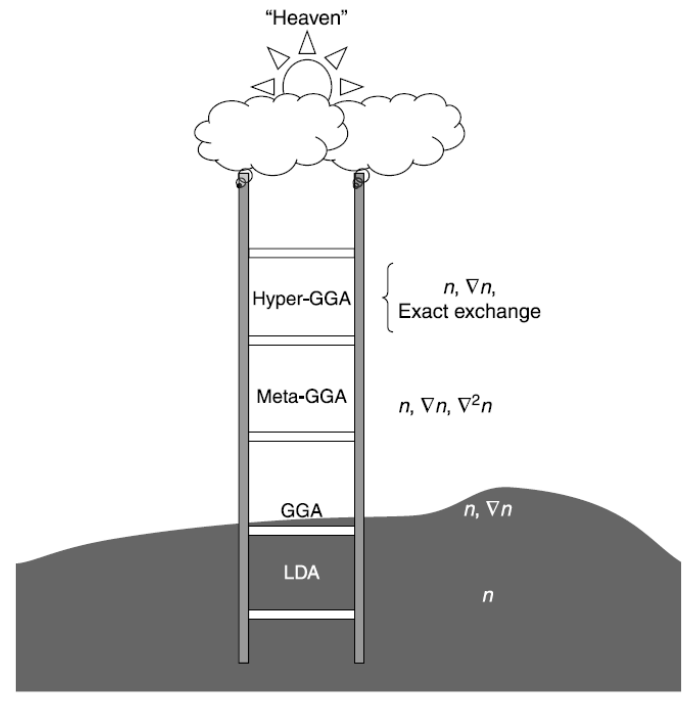
\includegraphics[height=3.4in,width=3.18in,viewport=10 5 680 700,clip]{Jacobi-ladder.png}
\caption{\small The schematic digram of Jacob's Ladder for DFT.\cite{Perdew-Schmidt_2001,Science298-759_2002}}
\label{Fig:Jacob-Ladder}
\end{figure}

上述{各类}泛函%的类别})
从上到下越来越接近%化学})
精确值,因此被形象地视为``Jacob's Ladder''(登天梯,见图\ref{Fig:Jacob-Ladder}):~将\textrm{LDA~}视为第一级阶梯,\textrm{GGA~}视为第二级阶梯,更复杂的泛函形式视为第三级及更高的阶梯。\cite{PRL91-146401_2003}但在密度泛函中过度引入轨道将会%造成})
{大大增加}计算量%的大大增加})
,失去密度泛函理论对%一般})
从头计算方法的优势,因此是{并}不可取的。
%下面对每一类中最重要的泛函作一些简单的介绍。
%
%\subsection{局域密度近似和LDA泛函}
%局域密度近似是Kohn和Sham提出的最简单的一种近似处理交换-相关能的方法。交换-相关能{泛函}的具体形式取为:
%\begin{equation}
%  \label{eq:dft-5}
%  E_{XC}^{\mathrm{LDA}}[\rho]=E_X^{\mathrm{LDA}}[\rho]+E_C^{\mathrm{LDA}}[\rho]=\int\varepsilon_X[\rho]\rho(\vec{r}) \textrm{d}^3\vec{r}+\int\varepsilon_C[\rho]\rho(\vec{r}) \textrm{d}^3\vec{r}
%\end{equation}
%其中$\varepsilon_X[\rho]$和$\varepsilon_C[\rho]$分别为{一个电子的}交换能和相关能%密度})
%。上式表明空间每一个点的交换能密度和相关能密度只是取决于该点的电子密度,而与其他点的电子密度无关。对{于均匀电子气,}$\varepsilon_X[\rho]$和$\varepsilon_C[\rho]$%的选取可按照均匀电子气中交换-相关能和电子密度的关系得到,})
%{为常数%,等于体系的总电子交换能(或相关能)除以体系的体积和电子密度
%。}对于非均匀电子气%而言})
%,%这样选取的$e_X(\rho)$和$e_C(\rho)$的物理图象相当于})
%{可以设想}把空间分割为无穷多个%非常})
%{无限}小的区域,%假设})
%{可以认为}电子的密度在每个小的区域内都是均匀的,每个小区域中的交换-相关能都%采用})
%{可以按}均匀电子气%模型下})
%的交换-相关能{计算},整个体系的交换-相关能就可以写成\eqref{eq:dft-5}式的形式。{采用}这种模型{,}%下的})
%\textrm{Kohn-Sham~}方程的交换势表达为:
%\begin{equation} \label{eq:dft-6}
%	V_X^{\mathrm{LDA}}(\vec{r}) =\dfrac {\delta E_X^{\mathrm{LDA}}}{\delta\rho(\vec{r}) }=-\dfrac 32\alpha\left\{\dfrac3\pi\rho(\vec{r}) \right\}^{1/3}
%\end{equation}
%Kohn和Sham等从总交换能的角度出发%给})
%{得}出$\alpha=2/3$\cite{PR140-A1133_1965},Slater从交换势的角度出发,%给})
%{得}出$\alpha=1$\cite{PR81-385_1951},对原子、分子体系的计算表明,选取$\alpha$约为0.7\cite{AQC6-1_1972,Slater-4_1974}结果更好。
%
%对于用自旋密度泛函方法处理的自旋极化体系%的情况})
%,%此时的})
%交换能{泛函的}形式可以写成\cite{PRA20-397_1979}
%\begin{equation} \label{eq:dft-7}
%E_X[\rho_{\alpha},\rho_{\beta}]=\frac12E_X^{0}[2\rho_{\alpha}]+\frac12E_X^{0}[2\rho_{\beta}]
%\end{equation}
%其中$E_X^{0}[\rho]=E_X\bigl[\dfrac 12\rho_{\alpha},\dfrac 12\rho_{\beta}\bigr]$
%
%相关能包含相同自旋电子间的相互作用和不同自旋电子间相互作用,不可能把相关能泛函也分解成为两种自旋电子的相关能的贡献和。一般采用Stoll\cite{TCA49-143_1978}的定义,将局域密度近似的相关能泛函写成如下形式:
%\begin{equation}
%  E_C=E_C^{\alpha\beta}+E_C^{\alpha\alpha}+E_C^{\beta\beta}
%  \label{eq:dft-17}
%\end{equation}
%
%把局域密度近似引入自旋密度泛函理论就是通常所说的局域{自旋}密度近似(local spin-density approximation, LSDA),LSDA中的交换能{泛函}%形})
%{表达}式可以%结合})
%{由}\eqref{eq:dft-7}式和\eqref{eq:dft-6}式%给})
%{得}出{。}相关能泛函的形式可以写成:
%$$E_C^{\mathrm{LSDA}}[\rho_{\alpha},\rho_{\beta}]=\int{\varepsilon_C(\rho,\varsigma)\rho\,\textrm{d}^3\vec{r}}$$
%其中$\varsigma=(\rho_{\alpha}-\rho_{\beta})
%/(\rho_{\alpha}+\rho_{\beta})
%$,$\rho_{\alpha}$和$\rho_{\beta}$分别是自旋为$\alpha$和自旋为$\beta$的电子密度。均匀电子气相关能的解析形式很难求得,但是可以用数值方法计算得到%其})
%数值结果,Vosko等\cite{CJP58-1200_1980}用解析式拟合%出})
%精确的数值计算结果,得到局域密度近似下的相关能泛函VWN表达式{。}%但是})
%他们给出的表达式%太})
%{比较}复杂,Perdew和Wang\cite{PRB45-13244_1992}%又})
%把它改%写})
%成%为})
%{比较}简单的形式,得到%的})
%{一个电子的}相关能%密度})
%{的}表达式为:
%\begin{equation}
%  \label{eq:dft-8}
%  \varepsilon_C^{\mathrm{LDA}}(r_s,\varsigma)=\varepsilon_C^{\mathrm{LDA}}(r_s,0)+a_C(r_s)\dfrac{f(\varsigma)}{f^{\prime\prime}(\varsigma)}(1-\varsigma^4)+[\varepsilon_C(r_s,1)-\varepsilon_C(r_s,0)]f(\varsigma)\varsigma^4
%\end{equation}
%其中$r_s=\left[\dfrac 3{4\pi}\bigl(\rho_{\alpha}+\rho_{\beta}\bigr)\right]^{-1/3}$,$f(\varsigma)=[(1+\varsigma)^{4/3}+(1-\varsigma)^{4/3}-2]/(2^{4/3}-2)$,\\$\varepsilon_C(r_s,0)$,$\varepsilon_C(r_s,1)$和$-a_C(r_s)$由经验公式
%$$G(r_s,A,\alpha_1,\beta_1,\beta_2,\beta_3,\beta_4,p)=-2A(1+\alpha_1r_s)\ln\left[1+\dfrac1{2A(\beta_1r_s^{1/2}+\beta_2r_s+\beta_3r_s^{3/2}+\beta_4r_s^{p+1})}\right]$$
%计算{,}其中{$G$可以是$\varepsilon_C(r_s,0)$,$\varepsilon_C(r_s,1)$或$-a_C(r_s)$},$A$,$\alpha_1$,$\beta_1$,$\beta_2$,$\beta_3$,$\beta_4$,$p$%都})
%是{特定的}参数。
%
%由于局域密度近似下的交换-相关能泛函形式是从均匀电子气模型中得到的,一般认为它对于电子密度变化比较小的体系结果比较好,%而})
%{可能}不适用于电子密度剧烈变化的原子、分子和一些固体体系。%事实上})
%{不过},局域密度近似用于原子、分子特别是某些扩展体系仍能得到很合理的结果,其原因是%因为})
%局域密度近似下的交换-相关能密度和交换-相关孔在每一点上的数值都来自一个体系的精确的值,因此满足交换-相关电荷总量为一个电子电荷的负值的约束条件,交换-相关能泛函的误差%在不同位置})
%{能部分}相互抵消。
%
%\subsection{梯度校正和GGA泛函}
%%由于})
%LDA是建立在均匀电子气模型基础上{的},而原子、分子和很多扩展体系的电子密度远非均匀,%通常})
%由LDA计算得到的分子的原子化能{通常}过大。%要})
%{为}进一步提高计算精度,%就})
%需要对电子密度的非均匀性加以校正。一般是通过在交换-相关能泛函中引入电子密度%的})
%梯度来加以校正{,}即构造GGA泛函。可以将GGA交换能泛函写成一般形式:
%\begin{equation}
%	E_X^{\mathrm{GGA}}=E_X^{\mathrm{\mathrm{LDA}}}-\sum_{\sigma}\int F[x_{\sigma}]\rho_{\sigma}^{\frac43}(\vec r)\textrm{d}^3r{=E_X^{\mathrm{LDA}}+E_X^{\mathrm{NL}}}
%  \label{eq:dft-18}
%\end{equation}
%其中$x_{\sigma}=|\nabla\rho_{\sigma}|\rho_{\sigma}^{-4/3}$称为约化梯度,是一个无量纲的量。%依据})
%{按}所用$F${泛函}的形式不同,%目前})
%{现有}GGA的交换能泛函可以分为两大类,一类以Becke\cite{PRA38-3098_1988}在1988年提出的表达式为基础:
%\begin{equation}
%  \label{eq:dft-9}
%  E_X^{\mathrm{NL}}=-b\sum_{\sigma}\int\rho_{\sigma}^{4/3}\dfrac{x_{\sigma}^2}{1+6bx_{\sigma}\sinh^{-1}x_{\sigma}}\textrm{d}^3r
%\end{equation}
%其中$b$\,=\,0.0042{。}%$X_{\sigma}=|\nabla\rho_{\sigma}|\rho_{\sigma}^{-4/3}$})
%这是目前常用的交换能非局域校正公式。属于这一类的交换能泛函有PW91\cite{PRB46-6671_1992,PRB48-4978_1993,PRB54-16533_1996,PRB57-14999_1998}、FT97\cite{MP91-847_1997}、CAM(A)和CAM(B)\cite{JCP99-8765_1993}等等。另一类泛函的$F${泛函}采用有理函数{形式,}包括幂函数和有理分式的泛函。属于这一类的交换能泛函有B86\cite{JCP84-4524_1986}、P86$_x$\cite{PRB33-8800_1986}、LG\cite{PRA47-4681_1993}、PBE\cite{PRL77-1396_1996,IBID78-1396_1997}、VSXC\cite{JCP109-400_1998}等。B86采用的$F${泛函}的形式是
%\begin{equation}
%	F^{\mathrm{B86}}=\left[1+1.296\left(\dfrac{x_{\sigma}}{(24\pi^2)^{1/3}}\right)^2+14\left(\dfrac{x_{\sigma}}{(24\pi^2)^{1/3}}\right)^4+0.2\left(\dfrac{x_{\sigma}}{(24\pi^2)^{1/3}}\right)^6\right]^{1/15}
%  \label{eq:dft-19}
%\end{equation}
%
%最常用的相关能非局域校正{$E_C^{\mathrm{NL}}$}是Perdew和Wang\cite{PRB33-8822_1986}提出的%形})
%{表达}式以及把$E_C^{\mathrm{NL}}$和$E_C^{\mathrm{LDA}}$合{并}在一起计算的LYP%形})
%{表达}式\cite{PRB37-785_1988}。Perdew和Wang的表达式为:
%\begin{equation} 
%  \label{eq:dft-10}
%  E_C^{\mathrm{NL}}=\int{d^{-1}\textrm{e}^{-\varphi}C[\rho]|\nabla\rho|^2\rho^{-4/3}\textrm{d}^3r}
%\end{equation}
%其中$\varphi=1.745\times 0.11\times C[\infty]|\nabla\rho|/(C[\rho]\rho^{7/6})$,%\\%\linebreak
%
%$d=2^{1/3}\left[\biggl(\dfrac {1+\varsigma}2\biggr)^{5/3}+\biggl(\dfrac{1-\varsigma}2\biggr)^{5/3}\right]^{1/2}$,
%
%$C[\rho]=a+(b+ar_s+\beta r_s^2)(1+\gamma r_s+\delta r_s^2+10^4\beta r_s^3)^{-1}$,\\%\linebreak
%$a$,$b$,$\alpha$,$\beta$,$\gamma$,$\delta$为通过拟合{实验数据}得到的参数。
%
%LYP相关能泛函是%利用})
%{在}Colle-Salvetti公式\cite{TCA37-329_1975}{的基础上}导出的,其具体形式为:
%\begin{equation}
%  \begin{aligned}
%	  E_C^{\mathrm{LYP}}=&-a\int\dfrac{\gamma(\vec r)}{1+d\rho^{-1/3}}\biggl\{\rho+2b\rho^{-5/3}\biggl[2^{2/3}C_F\rho_{\alpha}^{8/3}+2^{2/3}C_F\rho_{\beta}^{8/3}-\rho t_w\biggr.\biggr.\\
%  &+\left.\left.\dfrac19\left(\rho_{\alpha}t_w^{\alpha}+\rho_{\beta}t_w^{\beta}\right)+\dfrac1{18}\left(\rho_{\alpha}\nabla^2\rho_{\alpha}+\rho_{\beta}\nabla^2\rho_{\beta}\right)\right]\textrm{e}^{-c\rho^{-1/3}}\right\}\textrm{d}\vec r
%  \end{aligned}
%  \label{eq:dft-20}
%\end{equation}
%其中$\gamma(\vec r)=2\left[1-\dfrac{\rho_{\alpha}^2(\vec r)+\rho_{\beta}^2(\vec r)}{\rho^2(\vec r)}\right]$,$t_w(\vec r)=\dfrac18\cdot\dfrac{|\nabla\rho(\vec r)|^2}{\rho(\vec r)}-\dfrac18\nabla^2\rho(\vec r)$,$C_F=\dfrac3{10}(3\pi^2)^{2/3}$,\\$a$,$b$,$c$,$d$%是})
%{为通过拟合实验数据确定的}常数。
%
%\subsection{\textit{meta}-GGA泛函}
%由于密度泛函理论的交换-相关能中包含了实际体系与无相互作用参考体系动能{之}间的差别,%因此如果})
%在交换和相关能泛函中包含动能密度$\tau$,%则})
%计算结果可能会更合理一些。表达式中包含动能密度$\tau$为变量的泛函称为\textit{meta}-GGA泛函。动能密度的一般定义为
%\begin{equation}
%	\tau=\sum_i^{\mathrm{occ}}|\nabla\Psi_i|^2
%  \label{eq:dft-21}
%\end{equation}
%其中$\Psi_i$是含自旋的轨道。
%
%van~Voorhis和Scuseria于1998年提出了基于密度矩阵展开理论\cite{PRC5-1472_1972,PRC11-1031_1975}的VSXC泛函\cite{JCP109-400_1998},得到的交换能密度泛函为:
%\begin{equation}
%  \begin{aligned}
%    E_X[\rho_{\alpha},\rho_{\beta}]&=\sum_{\sigma}\int\rho_{\sigma}^{4/3}{f(x_{\sigma},z_{\sigma})
%    }\textrm{d}\vec r\\
%    f(x_{\sigma},z_{\sigma})&=\left(\dfrac a{\Gamma_{\sigma}(x,z)}+\dfrac{bx_{\sigma}^2+cz_{\sigma}}{\Gamma_{\sigma}^2(x,z)}+\dfrac{dx_{\sigma}^4+ex_{\sigma}^2z_{\sigma}+f_0z_{\sigma}^2}{\Gamma_{\sigma}^3(x,z)}\right) 
%  \end{aligned}
%  \label{ed:def-22}
%\end{equation}
%其中$x_{\sigma}=|\nabla\rho_{\sigma}|\rho_{\sigma}^{-4/3}$,$z_{\sigma}=\tau\rho_{\sigma}^{-5/3}-C_F$,$C_F=\dfrac35(3\pi^2)^{2/3}$,$\Gamma_{\sigma}(x,z)=1+\alpha(x_{\sigma}^2+z_{\sigma})$,\linebreak $\alpha$为常数;$a$,$b$,$c$,$d$,$e$,$f_0$均为参数。
%
%{在}相关能泛函的计算中,将相同自旋电子的相关作用和不同自旋{电子}的相关作用分开%计算})
%{处理}\cite{TCA49-143_1978},%有})
%\begin{equation}
%  \begin{aligned}
%    E_C=&E_C^{\alpha\beta}+E_C^{\alpha\alpha}+E_C^{\beta\beta}\\
%    E_C^{\sigma\sigma^{\prime}}=&\int f^{\sigma\sigma^{\prime}}(x,z)e_{c\sigma\sigma^{\prime}}^{\mathrm{LDA}}\textrm{d}\vec r\\
%    E_C^{\sigma\sigma}=&\int f^{\sigma\sigma}(x_{\sigma},z_{\sigma})
%    D_{\sigma}e_{c\sigma\sigma}^{\mathrm{LDA}}\textrm{d}\vec r
%  \end{aligned}
%  \label{eq:dft-23}
%\end{equation}
%其中$x^2=x_{\alpha}^2+x_{\beta}^2$,$z=z_{\alpha}+z_{\beta}$,{$e_C^{\mathrm{LDA}}$为相关能密度,}$D_{\sigma}$是相同自旋自相互作用的校正系数,表达式为:
%$$D_{\sigma}=1-\dfrac{x_{\sigma}^2}{4(z_{\sigma}+C_F)}$$
%
%1989年Becke和Roussel从类氢原子的密度矩阵表达式出发,提出%了})
%BR89交换能泛函\cite{PRA39-3761_1989}。
%交换势为:
%$$U_{X\sigma}=-4\pi\int_0^{\infty}\rho_X^{\mathrm{H}}(a,b,s)s\textrm{d}s=-\left(1-\textrm{e}^{-x}-\frac12x\textrm{e}^{-x}\right)/b$$
%其中$\rho_X^{\mathrm{H}}(a,b,s)$是类氢原子的交换孔函数,%$x$})
%{$x=ab$},由{逐点求解}超越方程
%$$\dfrac{x\textrm{e}^{-2/3}}{x-2}=\dfrac23\pi^{2/3}\dfrac{\rho_{\sigma}^{5/3}}{Q_{\sigma}}$$
%%逐点求解})
%得到。方程中$Q_{\sigma}$\,=\,$\dfrac16\left[\nabla^2\rho_{\sigma}-2\gamma\bigl(\tau_{\sigma}-\dfrac{(\nabla\rho_{\sigma})^2}{4\rho_{\sigma}}\bigr)\right]$,其中$\gamma$是参数,$\tau_{\sigma}$为动能密度{,}\linebreak $b$%根据})
%\,=\,$\left[\dfrac{x^3\textrm{e}^{-x}}{8\pi\rho_{\sigma}}\right]^{1/3}$%计算得到})
%{,$a=x/b$。}%最后得到})
%总的交换能为:$E_{X\sigma}=\dfrac12\displaystyle\int\rho_{\sigma}U_{X\sigma}\textrm{d}\vec r$
%
%对于分子体系,交换孔函数比较离域,BR89模型往往高估交换能密度,Becke用LDA动能与精确动能密度的比值为参数,提出了B00修正模型\cite{JCP112-4020_2000}。修正后的交换能泛函形式为:
%\begin{equation}
%	E_{X\sigma}^{\mathrm{BR89}}=\int e_{X\sigma}^{\mathrm{BR89}}[1+f_{X\sigma}(t_{\sigma})
%  ]\textrm{d}\vec r
%  \label{eq:dft-24}
%\end{equation}
%其中$f_{X\sigma}$是校正函数,$e_{X\sigma}^{\mathrm{BR89}}$是BR89模型中的交换能密度。$f_{X\sigma}(t_{\sigma})=a_t(\omega_{\sigma}-2\omega_{\sigma}^3+\omega_{\sigma}^5)$,$\omega_{\sigma}=\dfrac{t_{\sigma}-1}{t_{\sigma}+1}$,$t_{\sigma}=\dfrac{\tau_{\sigma}^{\mathrm{LSDA}}}{\tau_{\sigma}^{\mathrm{exact}}}$,式中$a_t$为经验参数。
%
%%若})
%加上{电子}相关{能}作用(采用Bc88相关能泛函\cite{JCP88-1053_1988})
%,得到的交换-相关能{泛函的}表达式为:
%\begin{equation}
%	E_{XC}=E_X^{\mathrm{BR89}}+c_{\mathrm{opp}}E_{C\mathrm{opp}}^{\mathrm{Bc88}}+c_{\mathrm{par}}E_{C\mathrm{par}}^{\mathrm{Bc88}}+a_{mix}\sum_{\sigma}\int e_x^{\mathrm{BR89}}f_{x\sigma}(t_{\tau})\textrm{d}\vec r
%  \label{eq:dft-25}
%\end{equation}
%其中$E_{C\mathrm{opp}}^{\mathrm{Bc88}}$和$E_{C\mathrm{par}}^{\mathrm{Bc88}}$分别是自旋平行、反平行的相关能。拟合得到的参数$a_{mix}$的优选值为0.135。
%
%\subsection{{杂化(hybrid)}泛函}
%%还有})
%{目前}一种很常用的交换-相关能{泛函}是%采用})
%把Hartree-Fock%的相关})
%{交换}能%形式})
%与近似%的})
%交换-相关能%相})
%混合%的方法})
%\cite{JCP104-1040_1996,JCP98-5648_1993},其表达式%可以写})
%为:
%\begin{equation}
%	E_{XC}^{\mathrm{hybrid}}=\alpha E_X+(1-\alpha)\bar{E}_X+\bar{E}_C
% \label{eq:dft-11}
%\end{equation}
%其中$E_X$是Hartree-Fock%的相关})
%{交换}能%形式})
%,$\bar{E}_X$和$\bar{E}_C$分别为近似的交换能和相关能泛函,通常$\alpha$取值为0.28左右。%例如})
%“半对半(half and half)”泛函\cite{JCP98-1372_1993}%,其})
%{的}表达式%可以写成})
%{为}:
%\begin{equation}
%	E_{XC}^{\mathrm{HH}}=\dfrac12E_{X}^{\mathrm{HF}}+\dfrac12E_{XC}^{LSDA}
%  \label{eq:dft-26}
%\end{equation}
%
%杂化型的密度泛函方法可以统一地归为一类,称为绝热关联方法(Adiabatic Connection Method, ACM)。所谓绝热关联,就是定义以$\lambda$为参量的Hamiltonian
%\begin{equation}
%  \hat H_{\lambda}=-\dfrac12\sum_i\nabla_i^2+\sum_iV_i(\rho,\lambda)+\dfrac{\lambda}2\sum_{i\neq j}\dfrac1{r_{ij}}
%  \label{eq:dft-27}
%\end{equation}
%其中$V_i(\rho,\lambda)$是与$\lambda$有关的外势,选择$V_i(\rho,\lambda)$使不同$\lambda$时的密度$\rho$保持恒定。%显然})
%当$\lambda$=0时对应于无相互作用参考体系;而当$\lambda$=1时对应%着})
%真实体系。当$\lambda$连续地从0变化到1时,无相互作用参考体系绝热地过渡到真实体系。利用一级微扰理论\cite{JCP88-1053_1988},可以得到交换-相关能%地})
%{的}表达式为:
%$$E_{XC}=\dfrac12\int\rho(\vec r)d\vec r\int\dfrac{\bar h_{xc}(\vec r,\vec r\,^{\prime})}{|\vec r-\vec r\,^{\prime}|}\textrm{d}\vec r\,^{\prime}$$
%其中$$\bar h_{xc}(\vec r,\vec r\,^{\prime})=\int_0^1h_{xc}^{\lambda}(\vec r,\vec r\,^{\prime})\textrm{d}\lambda$$
%$h_{xc}^{\lambda}(\vec r,\vec r\,^{\prime})$是与$\hat H_{\lambda}$相应的交换-相关孔函数。令
%$$U_{XC}^{\lambda}=\dfrac12\int\rho(\vec r)d\vec r\int\dfrac{h_{xc}^{\lambda}(\vec r,\vec r\,^{\prime})}{|\vec r-\vec r\,^{\prime}|}\textrm{d}\vec r\,^{\prime}$$
%于是有$$E_{XC}=\int_0^1U_{XC}^{\lambda}\textrm{d}\lambda$$
%如果%选用最})
%简单%的})
%{地}假设,%认为})
%$U_{XC}^{\lambda}$与$\lambda$满足线性关系,就%可以})
%得到
%$$E_{XC}=\dfrac12U_{XC}^0+\dfrac12U_{XC}^1=\dfrac12E_X^{HF}+\dfrac12U_{XC}^1$$
%这就是“半对半(half and half)”泛函以及%所有})
%{其它}杂化型泛函的理论基础。
%
%属于这一类的泛函还有B3P\cite{JCP98-5648_1993}、B3LYP\cite{JPC98-11623_1994}、B1B95\cite{JCP104-1040_1995}、B97\cite{JCP107-8554_1997}、B98\cite{JCP109-2092_1998}、PBE0\cite{JCP110-6158_1999}~等。其中最流行的B3LYP泛函的具体形式为:
%$$E_{XC}^{\mathrm{B3LYP}}=(1-a)E_X^{\mathrm{LSDA}}+aE_X^{\mathrm{HF}}+bE_X^{\mathrm{B88}}+cE_C^{\mathrm{LYP}}+(1-c)E_C^{\mathrm{LSDA}}$$
%其中$a$,$b$,$c$%均})
%为参数。
%
%%一般来说})
%这几种泛函的近似公式的计算结果{一般}差别并不很大,对各种近似泛函的计算结果可以参考文献\inlinecite{JCP98-5612_1993,CPL316-160_2000}。
%

由于原子中的电子密度的不均匀性比分子中的不均匀性更强,交换-相关能的梯度校正部分对原子{计算}影响比较大,%能够})
比较明显%的})
{地}降低原子的能量,而对分子{计算}影响较小{。}与LDA的结果相比,交换-相关能的梯度校正使得分子的原子化能{计算值}降低,键长{计算值}增加,总体%上得到的})
{看计算}结果%也})
有明显改善。%也正是这些})
精度较高的交换-相关能泛函%形式})
的提出,使%得})
密度泛函理论%能够广泛应用于定量研究})
{在}原子、分子、团簇和固体等%各种})
体系的%性质。})
{定量研究中得到广泛的应用并且得到满意的结果。}

\subsection{近似能量泛函的主要问题}
有必要指出的是,目前使用的{近似能量}泛函%形式})
还存在问题,比较集中的有:
\begin{enumerate}
	\item 自相互作用抵消不干净;
	\item 对于简并基态和近简并基态还存在%严重问题})
{难于合理解决的困难};
	\item 对于弱相互作用体系,如van der Waals相互作用不能忽略时,{计算结果}还有很大的误差。%由于})
\end{enumerate}
电子与{其}自身没有相互作用,因此交换-相关能中包含的电子自相互作用部分应该和电子间Coulomb能中包含的自相互作用部分完全抵消,而目前使用的{近似能量密度}泛函%形式})
都不%具有})
{严格满足}这个%特点})
{条件},因此{用}密度泛函方法计算电子数很少的体系一般都会有比较大的误差。{在体系处于}简并基态和近简并基态的%问题一直是密度泛函理论比较困难的部分})
{情况下},当%体系的})
基态电子密度%取自})
{用}不同的简并轨道{计算}时%密度泛函方法得到的})
体系能量应该%保持一致})
{不变},%现在的})
{而现有近似能量密度}泛函%形式也})
不具有这个%特点})
{性质},%由于多数原子的基态是简并的,})
用%密度泛函方法})
{来}计算%的})
原子基态能量就%会})
随%着选})
取%的})
不同简并原子轨道{计算电子密度}而不同\cite{PRB43-6865_1991,CPL265-481_1997},%这})
给计算分子体系的原子化能造成很大%的})
困难。密度泛函方法计算弱相互作用体系出现%问题})
的{困难}主要%原因})
是弱相互作用体系%通常键})
{中的相互作用}能和现%在所用的近似泛函形式})
{有近似能量密度泛函}本身的{计算}误差%可以相比})
{在同一量级}。%但是})
寻找精度%有})
明显提高的近似能量密度泛函%形式})
是难度很大的工作,目前常用的{近似能量密度}泛函%形式})
主要是二十世纪八十年代后期和九十年代初提出的,此后虽然%也有一些})
{提出过很多}近似{能量密度}泛函%形式被提出来})
,%但是})
与以前提出的%泛函形式})
相比%都})
{精度并}没有很明显的%改进})
{提高}。

\noindent{\heiti{习题}}\\
1. 简述\textrm{Hohenberg-Kohn}定理的基本内容并推导证明过程.\\
2. 基于\textrm{Kohn-Sham}方程,写出密度泛函理论的体系总能量表达式(提示:~将体系动能用Kohn-Sham方程本征态表示),并在此基础上讨论\textrm{Kohn-Sham}方程中的``交换-相关势''与体系总能表达式中``交换-相关能''的联系与区别.\\
3. 借助参考文献,熟悉常见\textrm{L(S)DA}泛函和\textrm{GGA}泛函的函数表达形式.%\\
%4. 推导精确泛函满足的交换-相关孔条件.

\section{第一原理计算方法简介}
能带理论是凝聚态物理中最重要的理论之一,它是量子力学确立后,在研究金属电导理论过程中发展起来的,已经成为固体电子理论的支柱。理想晶体的原子有序排列形成晶格,具有平移周期性,%势能$V(\vec r)$满足:
%\begin{equation}\label{eq:solid-2}
%	V(\vec r)=V(\vec r+\vec R_n)\quad\mbox{($\vec R_n$为任意格矢)}
%\end{equation}
%\textrm{Bl\"och}定理指出:
%{\it 对于具有周期性的势场,单电子的Schr\"odinger方程}
%\begin{equation}\label{eq:solid-1}
%  \biggl[-\dfrac{\hbar^2}{2m}\nabla^2+V(\vec r)\biggr]\psi=E\psi
%\end{equation}
%{\it 的解满足}
%\begin{equation}
%  \psi(\vec r+\vec R_n)=e^{i\vec k\cdot\vec R_n}\psi(\vec r)
%  \label{eq:bloch}
%\end{equation}
%$k$是与平移对称性相应的量子数,因此理想晶体的
根据能带理论,电子波函数具有与势函数相同的平移周期性,并且受到平面波的相位控制。密度泛函理论发展起来后,为电子结构模拟奠定了的基础,选定合适的交换-相关泛函(主要是LDA或GGA),在倒空间内自洽迭代求解Kohn-Sham方程,即可得到电子能带。应用DFT求解能带结构时,除了泛函的选择,还需要考虑的问题主要包括:
\begin{itemize}
	\item 周期性势函数的表示
	\item 周期体系的总能计算包括无限原子(或离子)的求和,要考虑发散级数的处理
	\item 不同的实现方案的区别,主要源于基函数形式的不同
\end{itemize}

\subsection{Muffin-Tin近似与非Muffin-Tin校正}
周期体系的势函数与一般原子、分子的差别,主要表现在原子间区域,相应部分的波函数较为平缓,并且有周期特征,如图\ref{Potential-Wave}所示:
\begin{figure}[h!]
\centering
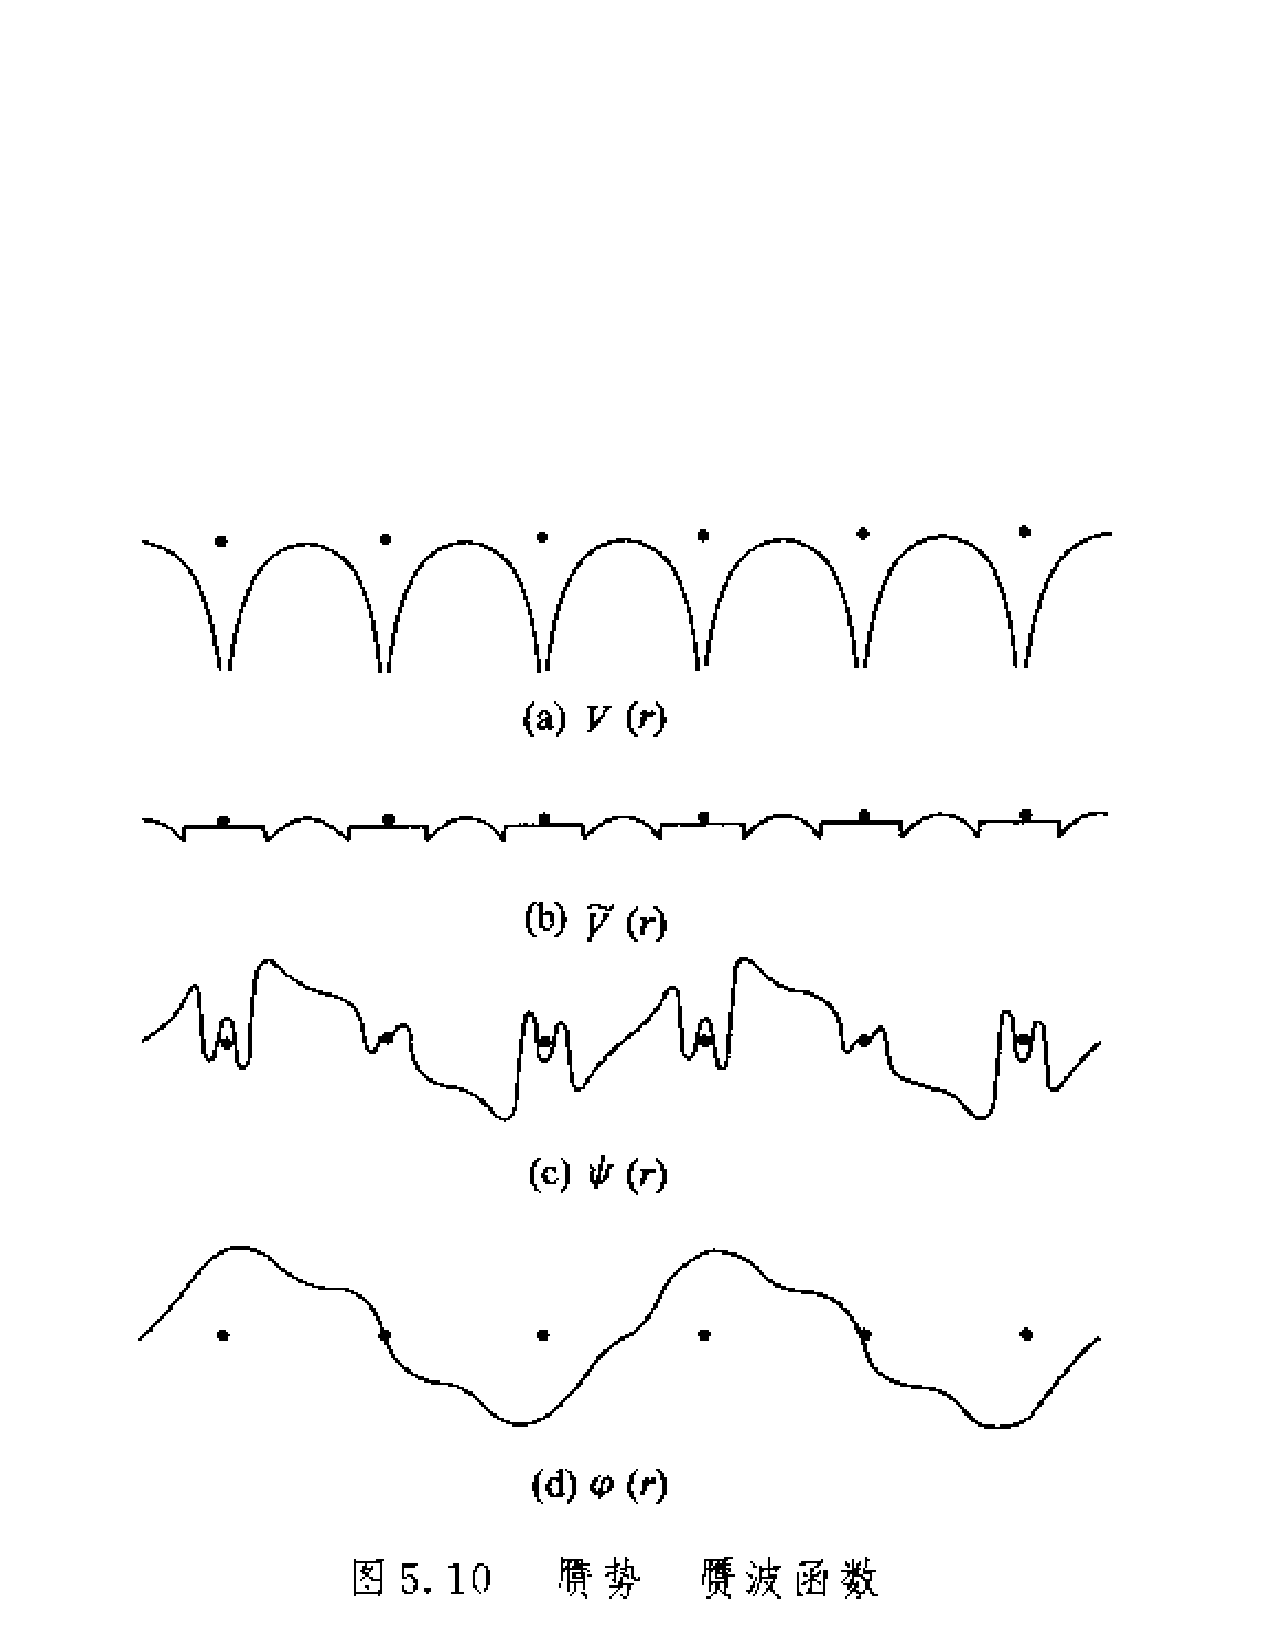
\includegraphics[height=0.8in,width=4.in,viewport=41 458 539 546,clip]{Pseudo_wave.pdf}\\
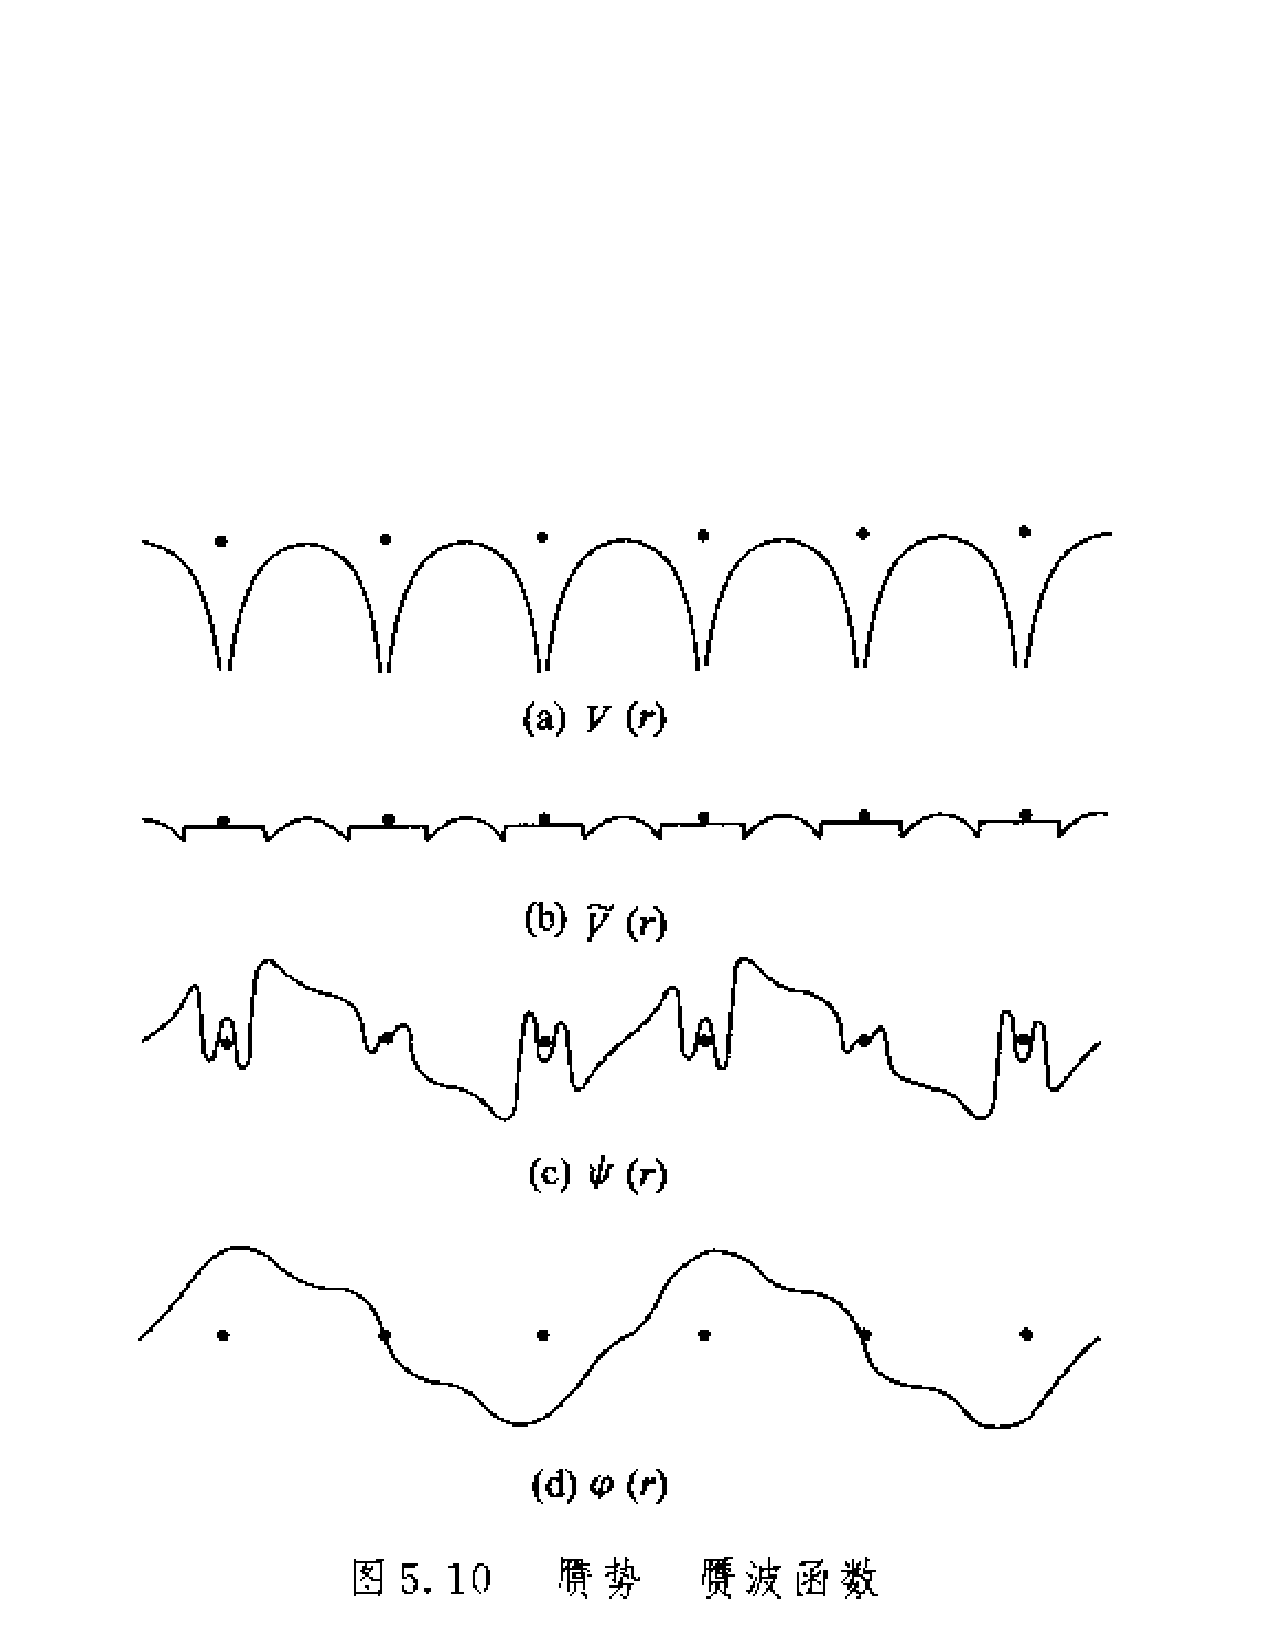
\includegraphics[height=0.8in,width=4.in,viewport=41 238 539 339,clip]{Pseudo_wave.pdf}
\caption{\small \textrm{The periodic Potential (up) and the wave functions (down) in crystal.}}%(与文献\cite{EPJB33-47_2003}图1对比)
\label{Potential-Wave}
\end{figure}

最早的能带计算方法是Wigner-Seitz(WS)原胞方法\cite{PR43-804_1933}。该方法不考虑晶体对称性特征,将原胞简化为球,假定原胞势场仍保持球对称性,结果仅依赖于每个原胞平均占据的体积,忽略实际晶体结构的影响。%即$V(\vec r)=V(r)$,波函数为中心力场Schr\"odinger方程标准的线性组合,边条件为$\left(\dfrac{\partial\psi_{\vec k}(r)}{\partial r}\right)_{r_0}$,$r_0$为球半径。
\textrm{WS}原胞方法在碱金属能带计算取得了很大的成功,但由于模型过于简化,无法应用于大多数晶体的计算。%如果采用真实的多面体WS原胞,为了满足表面边边界条件,计算将变得十分复杂,同时也会导致中心力场在原胞边界上导数的不连续。
为了克服WS原胞方法的缺陷,Slater提出Muffin-Tin(MT)近似\cite{PR51-846_1937}。MT近似的主要思想是将WS原胞分为两个区域:~以原胞中的每个原子{\it i}\,为中心,半径为$r_i$的彼此不相交叠的球形区,此区域内势函数具有球对称性;球形区以外为间隙区,此处势能近似为一常数。
如图\ref{Muffin_tin-1}所示:
\begin{figure}[h!]
\centering
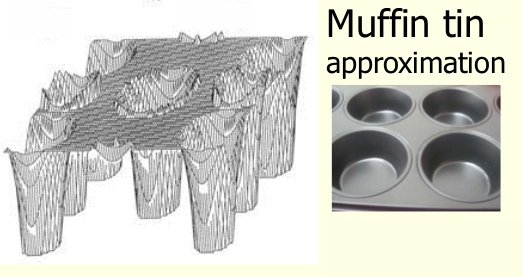
\includegraphics[height=1.45in,width=1.92in,viewport=1 22 317 295,clip]{Muffin-tin.png}
%\includegraphics[height=1.45in,width=1.92in,viewport=1 20 515 435,clip]{Muffin-Tin.png}
\caption{\small \textrm{Division of the unit cell into spheres(I) and into interstitial region(II)}}%(与文献\cite{EPJB33-47_2003}图1对比)
\label{Muffin_tin-1}
\end{figure} 

用数学形式表示即为:
\begin{equation}
  V(\vec r)=\left\{
  \begin{aligned}
    &V(|r|),\quad&r\leqslant R_{MT} \\
    &V_c.&r>R_{MT}
  \end{aligned}\right.
  \label{eq:Muffin-Tin}
\end{equation}
%为简化计算,
通常取$V_c$=0,这等价于将晶体的势能零点移动到$V_c$位置上。

MT势比WS原胞法相更接近实际情况,适用性更强。研究表明,对于过渡金属和具有密堆积结构的过渡金属化合物,间隙区势能近似为常数,MT方法是很好的近似,计算结果只会有很小的误差\cite{PR153-931_1967,PRB1-1318_1970,PLA33-414_1970}。%计算也表明, 
即使对于晶体势场不能完全用MT势描述的情况,如球内的非球形对称部分不能完全忽略的情况,也可以通过适当的方法修正。

%为了计算周期性晶体势场,Mattheiss提出了一个构造MT势的方法,在中心原子的势场上叠加上周围原子势场以中心为原点的球谐函数展开的球对称部分\cite{PRA133-1399_1964}。将Coulomb势和交换项分开处理。Coulomb势用晶体中原子势的静电排斥叠加表示,临近原子的Coulomb势叠加用L\"owdin发展的$\alpha$展开方法计算:
%\begin{equation}
%  V_C(r)=\sum_i\dfrac{N_i}{2a_ir}\int_{|a_i-r|}^{|a_i+r|}r'V_C^{at}(r')dr'
%  \label{eq:lodin-alpha}
%\end{equation}
%其中$a_i$是第$i$个等同原子球的半径;$N_i$是第$i$个原子的等同原子球数目;$V_C^{at}(r)$是原子的Coulomb势,可用下式%\eqref{eq:atomic-coulomb}
%计算:
%\begin{equation}
%  V_C^{at}(r)=-\dfrac{2Z}r+\frac2r\int_0^r4\pi\rho^{at}(r')r'^2dr'+2\int_r^{\infty}4\pi r'\rho^{at}(r')dr'
%  \label{eq:atomic-coulomb}
%\end{equation}
%其中$\rho^{at}(r)=\sum\limits_l n_lu_l^2$是自洽的原子电荷密度,$n_l$是占据电子数,$u_l$是自洽原子波函数\cite{Herman-Skillman}。对于含有重元素的体系,$u_l$的计算可参考文献\inlinecite{PR137-23_1965}。由此得到的MT势为
%\begin{equation}
%  V_{MT}(r)=V_C^{at}(r)+\sum_i\dfrac{N_i}{2a_ir}\int_{|a_i-r|}^{|a_i+r|}r'V_C^{at}(r')dr'+V_{xc}(r)-V_c
%  \label{eq:potential-MT}
%\end{equation}
%最初的交换势$V_{xc}$贡献用Slater的$\chi_{\alpha}$方法计算\cite{PR81-385_1951},现在则根据选定的交换-相关泛函给出。计算时$\rho(r)$取晶体的空间电荷密度,初始值为中心原子的电子密度叠加相邻原子的电子密度。$V_c$是MT球间常数势。对单原子金属体系,WS原胞内的MT球间常数势为
%\begin{equation}
%  V_c=\dfrac3{R_{WS}^3-R_{MT}^3}\int_{R_{MT}}^{R_{WS}}V_{MT}(r)dr
%  \label{eq:monoatomic-ini}
%\end{equation}
%这里$R_{WS}$由$(4/3)\pi R_{WS}^3=\Omega_0$计算得到,$\Omega_0$是原胞体积。

%MT近似方法主要适用于具有密堆积的简单晶格的单原子(过渡)金属\cite{SSP26-104_1971},但对于非密堆积的金属化合物(如体心立方的CsCl结构)\cite{PRB13-5362_1976}的计算结果不理想,因为在化合物中原胞电中性条件无法保证。对于这类含有复式晶格的体系,必须采用另外的方法计算\cite{PSSB36-447_1969}。
%与简单晶格计算方法相比,复式晶格计算中叠加的是位于不同中心的电子密度而不再是原子势,并利用元胞的电中性假设,求出MT球间的常数电荷。确定电荷密度之后,利用Poisson方程求解MT球内势能和球间的常数势$V_c$。

%复式晶格的电子密度表示
%\begin{equation}
%  \rho_s(r)=\rho_s^{at}(r)+\sum_{mj}\dfrac{n_{mj}}{2a_{mj}r}\int_{|a_{mj}-r|}^{|a_{mj}+r|}\rho_m^{at}(r')r'dr'
%  \label{eq:equation-58}
%\end{equation}
%这里$\rho_s^{at}(r)$是$s$原子的电子密度;$r=|\vec r-\vec{\tau}_j|\leqslant R_{MT}^s$;$\vec{\tau}_j$是第$j$个等同原子球心位置;$n_{mj}$是中心在$\tau_j$矢径为$a_{mj}$的等同原子$m$的数目。WS原胞MT球外的常数电荷由复式原胞的电中性条件确定。
%\begin{equation}
%  \rho_c=\dfrac{\sum_i(Z_i-Q_i)}{\Omega_0-\sum_i\Omega_i}
%  \label{eq:solid-59}
%\end{equation}
%其中$Q_i=4\pi\int_0^{R_i}\rho_i(r)r^2dr$,$\Omega_i$是球心位于$\vec{\tau}_i$的球体积。在复式晶格内,根据周期性边界条件求解Poisson方程得到球对称晶体势,并对角度求和
%\begin{equation}
%  \begin{split}
%   V_s(r)=&-\frac{2Z_s}r+\frac{8\pi}r\int_0^r\rho_s(r')r'^2dr'+8\pi\int_r^{R_{MT}^s}\rho_s(r')r'dr' \\
%   &-2\sum_j(Z_j-Q_j+\rho_c\Omega_j)\varphi(\vec{\tau}_j-\vec{\tau}_s)-4\pi\rho_c(R_{MT}^s)^2 \\
%   &+\frac{(4\pi)^2}{3\Omega_0}\sum_j\int_0^{R_{MT}^s}[\rho_j(r')-\rho_c](r')^4dr'
%  \end{split}
%  \label{eq:solid-60}
%\end{equation}
%MT间的常数势根据式\eqref{eq:solid-61}确定:
%\begin{equation}
%  \begin{split}
%    V_c=&\frac2{\Omega_0-\sum_j\Omega_j}\left[\frac32\sum_j\frac{\Omega_j}{R_j}\left(Z_j-Q_j+\frac56\rho_c\Omega_j\right)\right.\\
%    &+\left.\sum_{ij}\Omega_j(Z_i-Q_i+\rho_c\Omega_i)\varphi(\vec{\tau}_i-\vec{\tau}_j)\right] \\
%    &+\frac{(4\pi)^2}{3\Omega_0}\sum_j\int_0^{R_{MT}^s}[\rho_j(r')-\rho_c](r')^4dr'
%  \end{split}
%  \label{eq:solid-61}
%\end{equation}
%这里$\varphi(\vec{\tau}_i-\vec{\tau}_j)$是位于$\vec{\tau}_j$的$j$离子静电势;$R_{MT}^s$是第$s$个MT球的半径。该球内的势能
%\begin{equation}
%  V_{MT}^s(r)=V_s(r)+V_{xc}(r)-V_c
%  \label{eq:solid-62}
%\end{equation}

%此外,晶体中离子(实)间的相互作用用Madelung势表示,对大多数晶体来说,晶体的Madelung势是已知的。需要指出的是,采用MT近似计算,正确选择MT球半径非常重要,因为球半径选择对于势能的Coulomb势和MT球内的电子电荷有重要影响。%对于WS原胞内含有两个原子的体系,MT球半径的选择使得两个MT球相切位置的MT势\eqref{eq:solid-62}相等。

使用MT近似方法,MT球外的势能是一常数,但实际上MT球外有非零的电子密度,%无法通过MT近似构造出与此电荷密度一致的势能。假设MT球外的电荷满足式\eqref{eq:solid-59},
间隙区的Coulomb势$V_c$并非是一常数,而与位置有关。所以应用MT近似,假设$V_c$为一常数,是MT近似误差的主要来源。 
%\subsection{非MT校正} %关于MT近似的改进方法有许多\cite{RPP44-139_1981},%考虑对MT近似的修正,主要有两类方案。一种是在推导Hamiltonian的基函数时考虑非MT效应;另一种采用MT近似构造基函数,但对势能进行非MT修正。一般来说主要应用第二种方案,构造一般形式的势能。在MT近似下,WS原胞分为球形区(S)和间隙区(I)两部分。对这两部分区域,由于表达形式的差别,
对不同区域的非MT校正,一般采用不同形式的校正形式:~在MT球内,晶体势用球谐函数(或者是满足晶体对称性的球谐函数),MT球外的势能用Fourier级数展开\cite{PRB13-5362_1976}
\begin{equation}
  V(\vec r)=\left\{
  \begin{aligned}
	  &\sum_LV_L(r)Y_L(\hat{\vec r}),\quad &r\leqslant R_{\mathrm{MT}}\\
	  &\sum_{\vec G_n}V_I(\vec G_n)e^{i\vec G_n\cdot\vec r},&r>R_{\mathrm{MT}}
  \end{aligned}\right.
  \label{eq:solid-63}
\end{equation}
这里$L\hat=l,m$,$\vec G_n$为倒格矢,$Y_L(\vec r)$是球谐函数。%这是合理的修正,因为靠近原子核,势能具有原子型势能特征。在MT球外,要求满足Bloch函数边界条件特征。由于MT球内外的势能表象不同,因此要求势能在MT球表面连续。
于是考虑修正后的晶体势为
\begin{equation}
	V(\vec r)=V_{\mathrm{MT}}(\vec r)+V_{\mathrm{WMT}}(\vec r)+V_{\mathrm{NS}}(\vec r)
  \label{eq:solid-64}
\end{equation}
这里$V_{\mathrm{MT}}(\vec r)$是简单的MT势;$V_{\mathrm{WMT}}(\vec r)$表示MT球外势能Fourier展开对MT近似常数势的偏离;$V_{\mathrm{NS}}(\vec r)$是式\eqref{eq:solid-63}第一个求和项中所有$\nu$$\neq$0之和。根据式\eqref{eq:solid-63},$V_{\mathrm{WMT}}(\vec r)$仅在MT球外贡献非零,球内为零;而$V_{\mathrm{NS}}(\vec r)$只在MT球内有非零值。一般$V_{\mathrm{WMT}}(\vec r)$比$V_{\mathrm{NS}}(\vec r)$大得多。

为求解交换-相关势$V_{xc}$,将电荷密度也用类似形式展开,代入交换-相关势表达式即可。
%\section{能带计算方法}
%晶体电子结构的计算可以分为两个部分:构造合理的具有平移周期性的晶体势场;在该势场下求解Schr\"odinger方程。不同的能带计算方法的主要区别在于:
%\begin{itemize}
%	\item 基函数的选取的不同
%	\item 根据研究对象性质的不同对晶体的势能作合理的近似
%\end{itemize}
%不同的计算方法,主要通过基函数为特征命名。

\subsection{基态总能量表达式}
%基态总能量表达式
在DFT框架内,周期体系的总能量$E_{\mathrm{T}}$由晶格中的电子能量$E_{\mathrm{e-e}}$与离子实排斥能$E_{\mathrm{N-N}}$之和\footnote{这部分主要参阅文献\inlinecite{XIE-LU}}:
	\begin{equation}
		E_{\mathrm{T}}=E_{\mathrm{e-e}}+E_{\mathrm{N-N}}=T[\rho]+E_{\mathrm{ext}}+E_{\mathrm{Coul}}+E_{XC}+E_{\mathrm{N-N}}
	\end{equation}
根据\textrm{Kohn-Sham}方程,其中动能泛函用单电子能量表示为
\begin{equation}
	T[{\rho}]=\sum_in_i\langle\psi_i|\varepsilon_i-V_{\mathrm{KS}}|\psi_i\rangle
\end{equation}
$n_i$是$\psi_i$上的电子占据数,$\varepsilon_i$是其能量本征值,因此有
\begin{equation}
	E_{\mathrm{T}}=\sum_in_i\varepsilon_i-\dfrac12\int\int\mathrm{d}\vec r\mathrm{d}\vec r\dfrac{\rho(\vec r)\rho(\vec r^{\prime})}{|\vec r-\vec r^{\prime}|}+\int\mathrm{d}\vec r\rho(\vec r)[\epsilon_{XC}(\vec r)-V_{XC}(\vec r)]+E_{\mathrm{N-N}}
	\label{eq:PP_TOT_R}
\end{equation}

周期体系的总能量表达式在动量空间($\vec K$空间)计算更方便
\begin{equation}
	E_{\mathrm{T}}=\sum_in_i\varepsilon_i-\dfrac{\Omega}2\sum_{\vec k\neq 0}\rho^{\ast}(\vec k)V_{\mathrm{Coul}}(\vec k)+\Omega\sum_{\vec k}\rho^{\ast}(\vec k)[\epsilon_{XC}(\vec k)-V_{XC}(\vec k)]+E_{\mathrm{N-N}}
\end{equation}
其中$V_{\mathrm{Coul}}(\vec k)$、$\epsilon_{\mathrm{XC}}(\vec k)$与$\rho^{\ast}(\vec k)$分别是\textrm{Coulomb}相互作用、单个电子的交换-相关能、交换-相关势和电子密度的\textrm{Fourier}分量。

电子间的\textrm{Coulomb}相互作用由\textrm{Poisson}方程计算
\begin{equation}
	\nabla^2V_{\mathrm{Coul}}(\vec r)=-4\pi\rho(\vec r)
\end{equation}
其\textrm{Fourier}展开为
\begin{equation}
	V_{\mathrm{Coul}}(\vec k)=\dfrac{4\pi\rho^{\ast}(\vec k)}{|\vec k|^2}
\end{equation}
显然,$V_{\mathrm{Coul}}(\vec k=0)$是发散的。

交换-相关势和交换-相关能的计算一般先在实空间计算$\epsilon_{XC}(\vec r)$和$V_{XC}(\vec r)$后,再通过\textrm{Fourier}变换到动量空间,得到$\epsilon_{XC}(\vec k)$和$V_{XC}(\vec k)$

离子间\textrm{Coulomb}相互作用能之和
\begin{equation}
	E_{\mathrm{N-N}}=\dfrac12\sum_{\vec R,s}\sideset{}{^{\prime}}\sum_{\vec R^{\prime},\vec s^{\prime}}\dfrac{Z_sZ_{s^{\prime}}}{|\vec R+\vec r_s-\vec R^{\prime}-\vec r_s^{\prime}|}
\end{equation}
这里$Z_s$是离子实的电荷数,$\vec R$表示晶格点的位矢,$\vec r_s$代表元胞内原子的相对位矢。$E_{\mathrm{N-N}}$求和包含无限多项,是发散的。
	
$V_{\mathrm{ext}}$在不存在其他外场时,一般只考虑离子-电子的\textrm{Coulomb}相互作用,
	\begin{equation}
		\begin{aligned}
			V_{\mathrm{ext}}(\vec r)&=\sum_{\vec R,s}\dfrac{-Z_s}{|\vec r-\vec R-\vec r_s|}\\
			&\equiv\sum_{\vec R,s}v_{\mathrm{ext}}^s(\vec r-\vec R-\vec r_s)
		\end{aligned}
	\end{equation}

	$V_{\mathrm{ext}}$的\textrm{Fourier}分量在$\vec k=0$也是发散的。因此基态总能量的表达式中存在三个发散项。因为整个体系是电中性的,意味着这些发散项会相互抵消,它们的和是一个常数\cite{JPC-SSP12-4409_1979}。因此周期体系总能量计算的一般流程为:~求解\textrm{Kohn-Sham}方程时,先将$V_{\mathrm{Coul}}(\vec k=0)$和$V_{\mathrm{ext}}(\vec k=0)$同时置为零,这相当于将势能作一平移,或者说重新定义势能零点,而在总能量计算中补偿这一平移。这样得到的发散项之和为:
	\begin{equation}
		\begin{aligned}
			\lim_{\vec k\rightarrow0}\Omega&\bigg[\dfrac12V_{\mathrm{Coul}}(\vec k)+\sum_sv_{ext}^s(\vec k)\bigg]\rho^{\ast}(\vec k)+\dfrac12\sum_{\vec R,s}\sideset{}{^{\prime}}\sum_{\vec R^{\prime},\vec s^{\prime}}\dfrac{Z_sZ_{s^{\prime}}}{|\vec R+\vec r_s-\vec R^{\prime}-\vec r_s^{\prime}|}\\
			=&\sum_s\alpha_s\sum_sZ_s+E_{\mathrm{Ewald}}
		\end{aligned}
	\end{equation}

对于形如$Z_s/r$的外场,其\textrm{Fourier}分量在$\vec k=0$附近展开
	\begin{equation}
		v_{\mathrm{ext}}^s(\vec k)=-\dfrac{4\pi Z_s}{\Omega|\vec k|^2}+\alpha_s+O(\vec k)
	\end{equation}
	展开$\rho^{\ast}(\vec k)$,有
	\begin{equation}
		\lim_{\vec k\rightarrow 0}\rho^{\ast}(\vec k)=\dfrac{\sum_sZ_s}{\Omega}+\beta|\vec k|^2+O(\vec k)
	\end{equation}
去掉高次项,有
\begin{equation}
	\begin{aligned}
		\lim_{\vec k\rightarrow 0}&\bigg[\dfrac{\Omega}2\dfrac{4\pi[\rho^{\ast}(\vec k)]^2}{|\vec k|^2}+\Omega\bigg(-\dfrac{4\pi\sum\limits_sZ_s}{\Omega|\vec k|^2}+\sum\limits_s\alpha_s\bigg)\rho^{\ast}(\vec k)+\dfrac12\dfrac{4\pi(\sum\limits_sZ_s)^2}{\Omega|\vec k|^2}\bigg]\\
		&+\dfrac12\sum_{\vec R,s}\sideset{}{^{\prime}}\sum_{\vec R^{\prime},\vec s^{\prime}}\dfrac{Z_sZ_{s^{\prime}}}{|\vec R+\vec r_s-\vec R^{\prime}-\vec r_{s^{\prime}}|}-\lim_{\vec k\rightarrow0}\dfrac12\dfrac{4\pi(\sum\limits_sZ_s)^2}{\Omega|\vec k|^2}\\
		=&\sum_s\alpha_s\sum_sZ_s+E_{\mathrm{Ewald}}
	\end{aligned}
\end{equation}

	\begin{equation}
		\begin{aligned}
			E_{\textrm{Ewald}}=&\dfrac12\sum_{\vec R,s}\sideset{}{^{\prime}}\sum_{\vec R^{\prime},\vec s^{\prime}}\dfrac{Z_sZ_{s^{\prime}}}{|\vec R+\vec r_s-\vec R^{\prime}-\vec r_{s^{\prime}}|}-\lim_{\vec k\rightarrow0}\dfrac12\times\dfrac{4\pi(\sum\limits_sZ_s)^2}{\Omega|\vec k|^2}\\
			=&\dfrac12\sum_{\vec R,s}\sideset{}{^{\prime}}\sum_{\vec R^{\prime},\vec s^{\prime}}\dfrac{Z_sZ_{s^{\prime}}}{|\vec R+\vec r_s-\vec R^{\prime}-\vec r_{s^{\prime}}|}-\dfrac1{2\Omega}\sum_{s,s^{\prime}}\int\mathrm{d}\vec r\dfrac{Z_sZ_{s^{\prime}}}r\\
			=&\sum_{s,s^{\prime}}Z_sZ_{s^{\prime}}\bigg\{\dfrac{2\pi}{\Omega}\sum_{\vec k\neq 0}\cos[\vec k\cdot(\vec r_s-\vec r_{s^{\prime}})]\dfrac{\mathrm{e}^{-|\vec k|^2/4\eta^2}}{|\vec k|^2}\\
			&-\dfrac{\pi}{2\eta^2\Omega}+\dfrac12\sum_{\vec R}\dfrac{\mathrm{erf}(\eta x)}x\bigg|_{\vec R+\vec r_s-\vec r_s^{\prime}\neq0}-\dfrac{\eta}{\sqrt{\pi}}\delta_{s,s^{\prime}}\bigg\}
		\end{aligned}
	\end{equation}
	$\mathrm{erf}(x)$是误差函数,$\eta$原则上是任意参数。$\alpha_s$由$v_{\mathrm{ext}}^s(\vec r)$确定:
	\begin{equation}
		\alpha_s=\lim_{\vec k\rightarrow0}\bigg[v_{\mathrm{ext}}^s(\vec k)+\dfrac{4\pi Z_s}{\Omega|\vec k|^2}\bigg]=\dfrac1{\Omega}\int\mathrm{d}\vec r\bigg[v_{\mathrm{ext}}^s(\vec r)+\dfrac{Z_s}r\bigg]
	\end{equation}

由此得到的总能量表达式是
\begin{equation}
	\begin{aligned}
		E_T=&\sum_i\varepsilon_i-\dfrac{\Omega}2\sum_{\vec k\neq0}\rho^{\ast}(\vec k)V_{\mathrm{Coul}}(\vec k)\\
		&+\Omega\sum_{\vec k}\rho^{\ast}(\vec k)[\epsilon_{XC}(\vec k)-V_{XC}(\vec k)]\\
		&+\sum_s\alpha_s\sum_sZ_s+E_{\mathrm{Ewald}}
	\end{aligned}
\end{equation}
%\begin{figure}[h!]
%\centering
%\vspace*{-0.18in}
%\includegraphics[height=1.85in,width=2.2in,viewport=0 0 600 495,clip]{Figures/VASP_Total_ENE.png}
%\caption{\small \textrm{The Total-E calculated by VASP.}}%(与文献\cite{EPJB33-47_2003}图1对比)
%\label{TOTEN_VASP}
%\end{figure}

%\subsection{正交平面波(Orthogonalized Plane Wave, OPW)方法}
%对于周期性体系,平面波$\exp[\mathrm{i}(\vec k+\vec G_i)\cdot\vec r]$是最简单的正交、完备基函数。原则上,晶体中单电子波函数(Bloch函数)总可以用平面波展开得到:
%\begin{equation}
%	\psi_i(\vec k,\vec r)=\frac1{\sqrt{N\Omega_0}}\sum_{\vec G_i}c_n(\vec k,\vec G_i)\exp[\mathrm{i}(\vec k+\vec G_i)\cdot\vec r]
%  \label{eq:solid-84}
%\end{equation}
%
%选用平面波作为基组的优点:
%\begin{itemize}
%	\item 具有较好的解析形式:正交归一化,无须考虑重叠积分。在大多数情况下, Hamiltonian矩阵元在平面波基组下有简单的解析表达式;
%	\item 原则上无穷多的平面波构成完备基组,可以通过增加平面波的数目,改善基组的性质;
%	\item 平面波基组是非定域的,即基组不依赖于原子的位置。
%\end{itemize}
%
%单纯的平面波基组应用到晶体结构计算中存在若干问题:%由于晶体波函数占有很宽的动量范围,
%在原子核附近,电子的动量很大,波函数表现出很强烈的振荡;在离原子核较远的区域,势能变化平缓,电子动量较小。因此如果采用平面波基组,既需要动量较小的也需要动量较大的平面波,电子波函数的平面波展开收敛得很慢。因此为了完成计算,必须采用很大一套的平面波基组。
%
%为了克服简单平面波基组的缺陷,Herring在1940年提出了正交平面波(OPW)方法\cite{PR57-1169_1940}。OPW的基本思想是:用原子的芯层电子波函数和平面波共同作为基组,并要求基函数与原子的芯层电子波函数构成的Bloch波函数正交,这样的基函数称为正交化平面波。
%
%OPW方法的基函数为:
%\begin{equation}
%	\varphi_i(\vec r)=\Omega_0^{-1/2}\mathrm{e}^{\mathrm{i}\vec k_i\cdot\vec r}-\sum_ca_c(\vec k_i)\chi_c(\vec k_i,\vec r)
%  \label{eq:OPW-set}
%\end{equation}
%这里$\vec k_i=\vec k+\vec G_i$。$\chi_c$是芯层电子的波函数。$\sum\limits_c$表示对所有芯层电子态求和。根据基函数与所有芯层电子态正交条件,
%%为保证基函数与所有芯层电子态正交,即
%%$$\int\varphi_i(\vec r)\chi_c(\vec k_i,\vec r)d\vec r\equiv\langle\varphi_i|\chi_c\rangle=0$$
%%由此确定正交系数$a_c(\vec k_i)$
%%$$a_c(\vec k_i)=\Omega_0^{-1/2}\int_{\Omega_0}\chi_c^{\ast}(\vec k,\vec r)e^{i\vec k_i\cdot\vec r}d\vec r$$
%%因此,
%正交化平面波可以表示为:
%\begin{equation}
%	\varphi_i(\vec r)=\Omega_0^{-1/2}\left[\mathrm{e}^{\mathrm{i}\vec k_i\cdot\vec r}-\sum_c\langle\chi_c(\vec k,\vec r),\mathrm{e}^{\mathrm{i}\vec k_i\cdot\vec r}\rangle\chi_c(\vec k,\vec r)\right]
%  \label{eq:solid-85}
%\end{equation}
%
%实际应用中,通常选择原子芯层Bloch波函数构造$\chi_c$。依照tight-binding近似\inlinecite{Huang-Han},
%$$\chi_c(\vec k,\vec r)=\Phi_{nlm,\vec k}(\vec r)=\frac1{\sqrt N}\sum_{n=1}^N\mathrm{e}^{\mathrm{i}\vec k\cdot\vec R_n}\Psi_{nlm}(\vec r-\vec R_n)$$
%这里N是晶体中所含原胞数目;$\Psi_{nlm}(\vec r)=u_{nl}(r)Y_{lm}(\hat{\vec r})$是孤立原子波函数。为了计算晶体势的Fourier分量$V(\vec k)$,将势能表示为各原子势能的求和,%:
%%\begin{equation}
%%  V(\vec r)=\sum_nV_{\alpha}(\vec r-\vec R_n)
%%  \label{eq:solid-86}
%%\end{equation}
%可有\cite{Euwema-Stukel-Collins}
%\begin{equation}
%  V(\vec k)=\frac1{\Omega_0}\left[\frac{8\pi}{|\vec k|^2}\left(-Z_a+4\pi\int\rho_a(r)j_0(kr)r^2dr\right)-4\pi\int_0^{\infty}V_{\chi_{\alpha}}^a(r)j_0(kr)r^2dr\right]
%  \label{eq:solid-87}
%\end{equation}
%这里交换-相关势用$\chi_\alpha$近似方法计算。显然$|\vec k|=0$点是势能奇点,将Bessel函数$j_0(kr)$展开为级数:
%$$j_0(kr)=1-\frac16(kr)^2+\cdots,$$可有:
%\begin{equation}
%  V(0)=-\frac{16}3\frac{\pi^2}{\Omega_0}\int_0^{\infty}\rho_a(r)r^4dr-\frac{4\pi}{\Omega_0}\int_0^{\infty}r^2V_{\chi_{\alpha}}(r)dr
%  \label{eq:solid-88}
%\end{equation}
%根据原胞的电中性条件,有$Z_a=4\pi\int\rho_a(r)r^2dr$。
%
%相比于其他方法,OPW方法的优势在于对晶体势能无须作任何近似,因此长于处理原胞内电荷密度分布具有较强各向异性的体系。实际上,在原子边界外,OPW方法与后面介绍的APW方法相似,两者都是将波函数用平面波展开;但是在原子边界内,OPW基组采用原子波函数和平面波的组合,不适用于含{\it d}\,和{\it f}\,轨道体系。OPW方法主要对于原子芯电子波函数彼此不重叠的体系有效。为了克服OPW方法难于处理含有{\it d}\,和{\it f}\,电子体系的问题,人们对OPW作了改进\cite{PR57-1169_1940,PR99-500_1955}。改进的思想是对OPW的基组作简单的改变,将靠近价层的{\it s}\,和{\it p}\,芯层波函数包括在尝试波函数的基组中。通过变分求得的久期方程解包括了靠近价带的芯层态。一般这些芯层能带都比较窄,引入的芯层{\it s}\,和{\it p}\,态可以近似为正确的波函数,这将有助于芯态的快速收敛。文献\inlinecite{PR164-993_1967}中,OPW方法用于计算Ni的能带结构。此后OPW方法推广到原胞中含有多个原子的体系并用于计算含有{\it d}\,和{\it f}\,轨道原子的化合物的能带结构\cite{PSSB94-51_1979,PSSB97-631_1980}。
%
%OPW方法的重要的不足是其基组的非正交性和过完备。因为基函数\eqref{eq:OPW-set}中,除了完备基组平面波外,还有成键态波函数的线性组合。因此OPW基组中部分基组将是线性相关,晶体的价电子波函数$\psi_k(\vec r)$展开将并不唯一。%为了消除OPW的这一不足,Girardeau提出了完全正交平面波(completely orthogonalized plane wave, COPW)的概念\cite{JMP12-165_1971}。COPW的主要思想是将基组的平面波空间$\{\vec K\}$划分为子空间$\{\vec k\}$和$\{\vec k_c\}$。COPW基组只限于子空间$\{\vec k\}$中,
%%\begin{equation}
%%  |\mathrm{COPW}(\vec k)\rangle=|\vec k\rangle-\sum_ca_{c\vec k}(|\chi_c\rangle-|\vec k_c\rangle)
%%  \label{eq:COPW-set}
%%\end{equation}
%%这里$|\vec k\rangle=\Omega_0^{-1}\exp(i\vec k\cdot\vec r)$;$\chi_c$是芯电子波函数。设$|\vec k|\gg k_{\mathrm F}(k_{\mathrm F}\mbox{是Fermi动量})$,正交系数$a_{c\vec k}=\langle\chi_c|\vec k\rangle$。一般地,COPW可以表示为某个线性算符$\mathbf L$作用于平面波:
%%\begin{equation}
%%  |\mathrm{COPW}(\vec k)\rangle=\mathbf L|\vec k\rangle
%%  \label{eq:solid-89}
%%\end{equation}
%%算符$\mathbf L$定义为
%%$$\mathbf L=\mathbf I-\mathbf S+\mathbf{SQ}$$
%%$\mathbf I$是单位算符;$\mathbf S=\sum\limits_c(|\chi_c\rangle-|\vec k_c\rangle)a_c$;$\mathbf Q=\sum\limits_c|\vec k_c\rangle\langle\vec k_c|$。当$\mathbf L$作用于子空间$\{\vec k\}$变换为COPW基函数空间($\vec k$),而子空间$\{\vec k_c\}$保持不动,$|\vec k_c\rangle$与芯态波函数$|\chi_c\rangle$对应。
%
%%COPW的基函数与OPW基函数类似,但是COPW的基函数是正交且线性无关的。
%%$$\langle\mathrm{COPW}(\vec k)|\mathrm{COPW}(\vec k')=\delta_{\vec k\vec k'}$$
%%由于COPW同样是完备基组,因此晶体的价电子波函数可以用COPW基唯一地展开为:
%%\begin{equation}
%%  \Psi_{\vec k}(\vec r)=\sum_iC(\vec k+\vec G_i)\mathbf L|\vec k+\vec G_i\rangle
%%  \label{eq:solid-90}
%%\end{equation}
%
%%与OPW方法相似,这种形式的COPW方法不适用于计算含有{\it d}\,和{\it f}\,电子结构体系。文献\cite{FMM50-928_1980}将COPW方法推广到过渡金属体系。所有的电子态被分为三组:(1)内层芯电子态;(2){\it d}\,外层芯电子态;(3){\it sp}\,-对称化价电子态。对过渡金属体系,COPW基组的形式为:
%%\begin{equation}
%%  \{\chi_c\}+\{\tilde d\}+\{\mathrm{COPW}(\vec k)\}
%%  \label{eq:solid-91}
%%\end{equation}
%
%%$\{\chi_c\}$是孤立离子内层芯电子态波函数构成的子空间$|\chi_c\rangle\equiv\Psi_{nl}(\vec r-\vec R_l)$;$|\chi_c\rangle$的中心位原胞中的不同格点,且彼此不重叠,即
%%\begin{equation}
%%  \int\Psi_{nl}^{\ast}(\vec r-\vec r_i)\Psi_{n'l'}(\vec r-\vec r_j)d\vec r=\delta_{ij}
%%  \label{eq:solid-92}
%%\end{equation}
%
%%$\{\tilde d\}$是正交归一化的{\it d}\,-态的过渡金属孤立离子的外层芯态。与内层芯态不同,晶体中位于不同格点金属离子的外层{\it d}\,电子的波函数彼此重叠,由不同格点的{\it d}\,轨道构造正交化的$|\tilde d\rangle$态
%%\begin{equation}
%%  |\tilde d_i\rangle=|d_i\rangle-\frac12\sum_j\beta_{ij}|d_j\rangle
%%  \label{eq:solid-93}
%%\end{equation}
%%这里$\beta_{ij}$是{\it d}\,-轨道的$\sigma$,$\pi$,$\delta$键重叠积分。式\eqref{eq:solid-93}对重叠积分精确到一阶,这一精度对全部过渡金属已经足够。$\{\mathrm{COPW}(\vec k)\}$在COPW子空间\eqref{eq:solid-89}表示。基组\eqref{eq:solid-92}是完全正交的,即:
%%\begin{equation}
%%  \begin{split}
%%    \langle\tilde d|\mathrm{COPW}(\vec k)\rangle\equiv0,\quad\langle\tilde d|\chi_c\rangle\equiv0,\quad\langle\chi_c|\mathrm{COPW}(\vec k)\rangle\equiv0\\
%%    \sum_{\vec k}|\mathrm{COPW}(\vec k)\rangle\langle\mathrm{COPW}(\vec k)|+\sum_d|\tilde d\rangle\langle\tilde d|+\sum_c|\chi_c\rangle\langle\chi_c|=1
%%  \end{split}
%%  \label{eq:solid-94}
%%\end{equation}
%%晶体价电子波函数用基函数表示为:
%%\begin{equation}
%%  \Psi_{\vec k}(\vec r)=\sum_iC(\vec k+\vec G_i)\mathbf L|\vec k+\vec G_i\rangle+\sum_{d_j}a_{d_j}(\vec k)|\tilde d_j\rangle
%%  \label{eq:solid-95}
%%\end{equation}
%%基组\eqref{eq:solid-91}也是过渡金属中引入赝势的有力工具。
%在后来的实际应用中,OPW方法很少直接作为基函数直接使用,但它几乎是其他方法的思想基础,特别是PAW方法,直接受到OPW方法的启发。
%
\subsection{计算方法简介}
\subsubsection{赝势(Pseudo Potential, PP)方法}
赝势方法是使用最多的计算晶体电子结构和物理性质的方法。1934年,Fermi为了解释碱金属的原子光谱的谱线移动提出了原子赝势的概念%(见图\ref{Pseudo-scatter-2})
\cite{NC11-157_1934,AJP52-695_1984},随后,Hellman等将赝势应用到原子和分子能级的描述\cite{JCP3-61_1935}%,见图\ref{Pseudo-scatter-2}
。
%\begin{figure}[h!]
%\centering
%\vspace*{-0.25in}
%\includegraphics[height=3.00in,width=4.54in,viewport=0 0 1150 750,clip]{Pseudo-scatter-2.png}
%\caption{{\textrm{Radial wave-function $\phi=r\psi$ for low-energy scattering as illustrated in a figure from the 1934 and 1935 papers of Fermi and coworkers for low-energy electron scattering from atoms and neutron scattering from nuclei.}}}%(与文献\cite{EPJB33-47_2003}图1对比)
%\label{Pseudo-scatter-2}
%\end{figure}

赝势理论的一个重要发展是在1960年前后,Phullips和Kleinman\cite{PR116-287_1959}在正交平面波(Orthogonalized Plane Wave, OPW)方法\cite{PR57-1169_1940}基础上导出赝势,广泛用于简单金属的能带计算。正交平面波的定义为:
\begin{equation}
	\psi_{\mathrm{OPW}}(\vec G)=\Phi_{\mathrm{PW}}(\vec G)-\sum_c\langle\chi_c|\Phi_{\mathrm{PW}}(\vec G)\rangle\chi_c,
  \label{eq:solid-108}
\end{equation}
这里$\chi_c$表示芯层波函数;$\Phi_{\mathrm{PW}}$是平面波。将式\eqref{eq:solid-108}代入Schr\"odinger方程,%$\mathbf H\Psi=E\Psi$,可得:
%\begin{equation}
%  \mathbf H\Phi-\sum_c\langle\chi_c|\Phi\rangle\mathbf H\chi_c=E\Phi-E\sum_c\langle\chi_c|\Phi\rangle\chi_c
%  \label{eq:solid-96}
%\end{equation}
并注意到芯层波函数$\chi_c$是$\mathbf H$的本征值$E_c$对应的本征态,可得平面波满足方程%方程\eqref{eq:solid-96}化为:
\begin{equation}
	\mathbf H\Phi_{\mathrm{PW}}+V_R\Phi_{\mathrm{PW}}=E\Phi_{\mathrm{PW}}
  \label{eq:solid-97}
\end{equation}
其中$V_R$可由等式
\begin{equation}
	V_R\Phi_{\mathrm{PW}}\equiv\sum\limits_c(E-E_c)\langle\chi_c|\Phi_{\mathrm{PW}}\rangle\chi_c
  \label{eq:solid-VR}
\end{equation}
确定。不难看出,$V_R$具有非局域算符的特征,%其作用于任意函数$f(\vec r)$上,有:
%\begin{equation}
%  \begin{split}
%    V_Rf(\vec r)&=\sum_c(E-E_c)\chi_c(\vec r)\int\chi_c^{\ast}(\vec r')f(\vec r')d\vec r'\\
%    &=\int V_R(\vec r,\vec r')f(\vec r')d\vec r'
%  \end{split}
%  \label{eq:solid-100}
%\end{equation}
%这里
\begin{equation}
	{\hat V}_R(\vec r,\vec r')=\sum_c(E-E_c)|\chi_c^{\ast}(\vec r')\rangle\langle\chi_c(\vec r)|
 \label{eq:solid-101}
\end{equation}
引入赝势$V_p$
\begin{equation}
  V_p=V(\vec r)+V_R
  \label{eq:solid-99}
\end{equation}
显然赝势$V_p$确定的Schr\"odinger方程的本征态是平面波
\begin{equation}
	(-\dfrac12\nabla^2+V_p)\Phi_{\mathrm{PW}}=E\Phi_{\mathrm{PW}}
  \label{eq:solid-98}
\end{equation}
并且赝势-平面波的本征值与真实电子态相同。%不难看出,赝势实际上是两部分势函数之和

在式\eqref{eq:solid-99}中,吸引势$V(\vec r)$是负值,势能$V_R$包含能量差$(E-E_c)$是正的,两个势能项相互抵消,这是赝势函数$V_p$比真实势$V(\vec r)$平缓得多的根源。当赝势函数的空间变化很小时,体系将回到近自由电子模型。因此赝势方法最重要的特点就是,只要构造的赝势合适,即可以通过少量平面波求解出体系的能量本征值,进而确定体系的性质。
%通过构造必要的赝势,求解本征方程,可以从第一原理求解能量$E(\vec k)$分布。但是这样的赝势方法相比OPW没有明显的优势。赝势方法由OPW变换得到,两者是完全等价的。因为需要求解非局域势$V_p(\vec r,\vec r',E)$,赝势方法求解过程比OPW方法更复杂。而且为了计算其他物理性质,必须根据求解的赝波函数得到真实的波函数。此外,根据OPW方法变换得到的赝势\eqref{eq:solid-99},其中$V_R$的表达式\eqref{eq:solid-101}并不唯一。%式\eqref{eq:solid-101}中的能量差$(E-E_c)$原则上可以用任意能量函数和指标$c$代替,即$f(E,c)$。
%赝势方程式\eqref{eq:solid-98}的能量本征值与真实的本征函数的解相同\cite{Harrison}。
值得注意的是,赝势的构造是不唯一的。在式\eqref{eq:solid-VR}定义的$V_R$,其不唯一性源于OPW基组的过完备性。这样得到的赝势一般称为经验赝势(参见图\ref{Pseudo_model-empty_core}),通常选择赝势的Fourier分量参数使得计算结果与实验一致。

在赝势方法发展的早期,广泛使用的赝势是基于实验数据提出的半经验模型赝势\cite{PM9-451_1964,PM12-529_1965,JPF2-270_1972,PRB11-2717_1975,PRB11-2726_1975,JPF6-L271_1976,PR174-769_1968}(参见图\ref{Pseudo-model})。此类模型赝势的一般形式为:
\begin{equation}
  V_p(q)=\frac{a_1}{q^2}[\cos(a_2q)+a_3]\exp(a_4q^4)
  \label{eq:solid-102}
\end{equation}
\begin{figure}[h!]
\centering
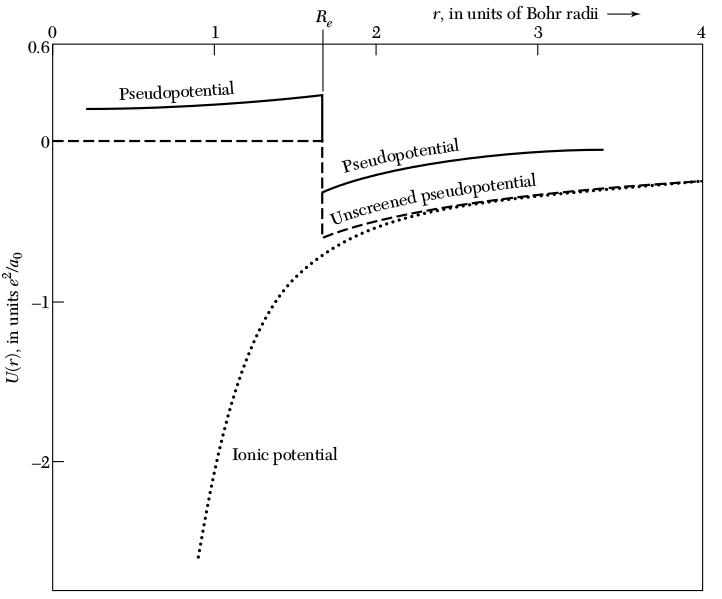
\includegraphics[height=1.60in,width=2.57in,viewport=0 0 980 600,clip]{Pseudo-model-empty_core.png}
\caption{\small \textrm{Pseudopotential for metallic sodium, based on the empty core model and screened by the Thomas-Fermi dielectric function.}}%(与文献\cite{EPJB33-47_2003}图1对比)
\label{Pseudo_model-empty_core}
\end{figure}
加入$\exp(a_4q^4)$因子使得可以适当选择$(a_4<0)$以保证这样赝势的Fourier展开很快收敛。常用半导体材料的赝势参数$a_i$可以从文献\inlinecite{PRB15-2154_1977}得到。这种形式的赝势通常称为软芯(softcore)势。%一般说,推导模型赝势要遵从如下三个原则:
%\begin{enumerate}
%  \item 要避免引入有大的散射动量$q(q\gg 2k_F)$的平面波作基函数(会引起收敛困难);%与离子赝势在正空间不连续有关。
%  \item 要考虑到赝势的非局域效应;
%  \item 为确定势能参数,尽量使用与金属性质没有直接关联的实验数据。
%\end{enumerate}
\begin{figure}[h!]
\centering
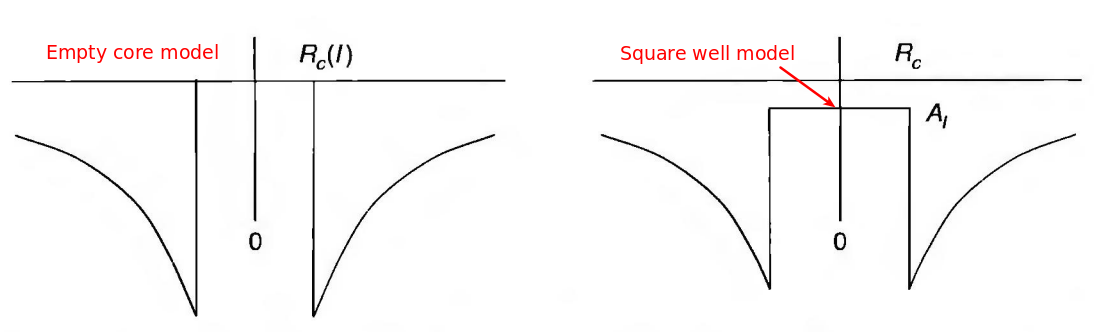
\includegraphics[height=1.30in,width=4.17in,viewport=0 0 1150 350,clip]{Pseudo-model.png}
\caption{\small \textrm{Left:``Empty core'' model potential of Ashcroft in which the potential is zero inside radius $R_c(l)$ which is different for each $l$. Right: Square well model potential with value $A_l$ inside a cut-off radius $R_c$, proposed by Abarenkov and Heine and fit to atomic data by Animalu and Heine..}}% The fact that the potential are weak, zero, or even positive inside cut-off radius $R_c$ is an illustration of the ``cancellation theorem''(与文献\cite{EPJB33-47_2003}图1对比)
\label{Pseudo-model}
\end{figure}

\subsubsection{模守恒赝势\textrm(Norm-Conserving Pseudo-Poential, NCPP)}
直接构造模型赝势的困难,限制了赝势方法的应用。随着密度泛函理论的兴起,通过构造和调节赝波函数(pseudo~wave),逆向求解径向Kohn-Sham方程来得到赝势,突破了赝势方法的应用瓶颈:
\begin{equation}
	\left[-\frac12\frac{\mathrm{d}^2}{\mathrm{d}r^2}+\frac{l(l+1)}{2r^2}+V(\rho,r)\right]P_{nl}(r)=\varepsilon_{nl}P_{nl}
  \label{eq:solid-103}
\end{equation}
这里$P_{nl}(r)$是构造的赝波函数的径向部分,一般包含多个可调参数;$V(\rho,r)$是自洽单电子势$$V(\rho,r)=-Z/r+V_{\mathrm{H}}(\rho,r)+V_{XC}^{\mathrm{LDA}}(\rho(r))$$
$V_{\mathrm{H}}(\rho,r)$是Hartree势,$V_{XC}^{\mathrm{LDA}}(\rho(r))$是LDA的交换-相关势。

这样得到的赝势称为第一原理赝势,赝势构造的重点由构造赝势本身转移到构造并选择合适的赝波函数。%目前主要的赝势方法主要都都是先构造赝函数,再通过径向方程\eqref{eq:solid-103}确定赝势。 
如果第一原理赝波函数满足以下条件\cite{PRB12-4200_1975,PRB18-5449_1978,PRB19-568_1979,PRB20-4082_1979,PRB26-4199_1982,PRL43-1494_1979,JPC13-L189_1980,PRB32-8412_1985,PRB43-1993_1991}:
\begin{itemize}
	\item 首先,赝波函数是平滑的且不含节点;
	\item 其次,在截断半径$r_{cl}$之外\cite{JPC13-L189_1980,PRB43-1993_1991},具有相同角动量$l$的原子径向赝波函数与全电子(all-electron, AE)波函数相等%即
\begin{equation}
	P_l^{\mathrm{PP}}(r)=P_l^{\mathrm{AE}}(r)\quad \mbox{满足}r>r_{cl}
  \label{eq:solid-104}
\end{equation}
%或者快速收敛到该值\cite{PRB18-5449_1978,PRL43-1494_1979,PRB32-8412_1985};
	\item 第三,赝波函数与全电子波函数在截断半径$r_{cl}$内的电荷密度相等\cite{PRL43-1494_1979,PRB43-1993_1991},
\begin{equation} 
	\int_0^{r_{cl}}|P_l^{\mathrm{PP}}(r)|^2\mathrm{d}r=\int_0^{r_{cl}}|P_l^{\mathrm{AE}}(r)|^2\mathrm{d}r
  \label{eq:solid-105}
\end{equation}
	\item 最后,全电子波函数和赝波函数对应的能量本征值相等,$e_l^{\mathrm{PP}}=e_l^{\mathrm{AE}}$。
\end{itemize}
这样构造的赝势称为模守恒赝势(norm-conserving pseudo~potential, NCPP)\cite{PRL43-1494_1979}。

实际应用模守恒赝势方法时,有很多方法可以构造出满足上述条件的赝波函数\cite{PRB18-5449_1978,PRB26-4199_1982,PRL43-1494_1979,JPC13-L189_1980,PRB32-8412_1985,PRB43-1993_1991},%得到赝波函数后,逆向求解径向Schr\"odinger方程,可以
通过式\eqref{eq:solid-103}直接得到的是屏蔽赝势:
\begin{equation}
	V_{\mathrm{src},l}^{\mathrm{PP}}(r)=\varepsilon_l-\frac{l(l+1)}{2r^2}+\frac1{2P_l^{\mathrm{PP}}(r)}\frac{\mathrm{d}^2}{\mathrm{d}r^2}P_l^{\mathrm{PP}}(r)
  \label{eq:solid-106}
\end{equation}
%从式\eqref{eq:solid-106}可见,因为赝波函数没有节点,赝势是平缓的,除了原子球心位置不再有其他奇点。图\ref{Pseudo-OPW_NCPP}给出的是模守恒赝势和\textrm{OPW}方法得到的赝势对应的3~\textit{s}~电子波函数的主要差别。
%\begin{figure}[h!]
%\centering
%\vspace*{-0.10in}
%\includegraphics[height=1.30in,width=4.17in,viewport=0 0 1150 350,clip]{Pseudo-OPW_NCPP.png}
%\caption{\small \textrm{Schematic example of a valence function that has the character of a $3s$ orbital near the nucleus and two examples of smooth functions (dashed lines) that equal the full wave-function outside the core region.}}% Left: the smooth part of the valence function defined by OPW-like equation; Right: a smooth pseudo-function that satisfies the norm-conservation condition.(与文献\cite{EPJB33-47_2003}图1对比)
%\label{Pseudo-OPW_NCPP}
%\end{figure}
这样得到的赝势包含当前环境的信息,%由价电子产生的屏蔽与其所处的环境有关,如果
为提高赝势对环境的适应性,尽可能减少当前环境对赝势的影响,可以扣除价电子屏蔽的贡献。%在自洽迭代过程中利用离子赝势得到特定环境的电子屏蔽。
通常的做法是从屏蔽赝势中减去与赝电荷密度(源于赝波函数)有关的Hartree势$V_{\mathrm{H}}^{\mathrm{PP}}(r)$和交换-相关势$V_{XC}^{\mathrm{PP}}(r)$%,即离子赝势\cite{PRB43-1993_1991}:
$$V_{\mathrm{ion},l}^{\mathrm{PP}}(r)=V_{\mathrm{src},l}^{\mathrm{PP}}(r)-V_{\mathrm{H}}^{\mathrm{PP}}(r)-V_{XC}^{\mathrm{PP}}(r)$$
这一过程称为赝势的去屏蔽。

有必要指出的是,这样得到的势函数是局域的,但它只是赝势的径向部分。考虑角度部分的贡献后,赝势函数表示为
\begin{equation}
	V_{\mathrm{ion}}^{\mathrm{PP}}=V_{\mathrm{ion},\mathrm{local}}^{\mathrm{PP}}(r)+\sum_lV_{\mathrm{nonlocal},l}(r)\hat P_l
  \label{eq:solid-107}
\end{equation}
等式右侧第一项$V_{\mathrm{ion},\mathrm{local}}^{\mathrm{PP}}(r)$是去屏蔽赝势的主要部分,它只依赖径向变量$r$,在整个空间都是局域的;第二项是赝势的角度相关部分,其中$V_{\mathrm{nonlocal},l}(r)=V_{\mathrm{ion},l}^{\mathrm{PP}}(r)-V_{\mathrm{ion},\mathrm{local}}^{\mathrm{PP}}(r)$,$\hat P_l$是Legendre多项式,表示角度部分的投影算符。由于角度部分无法完全分离变量,因此式\eqref{eq:solid-107}这种形式称为半局域赝势。半局域赝势在平面波基函数下计算复杂度为$O(N^3)$,具体计算中使用起来非常不便。

\textrm{Kleinman}和\textrm{Bylander}\textrm{(KB)}\cite{PRL48-1425_1982}针对半局域势引入变量可分离近似,并将赝势的球坐标表示变换到赝波函数空间,由此得到完全可分离赝势:
$$V_{\mathrm{nonlocal},l}^{\mathrm{KB}}=\sum_m\dfrac{|V_{\mathrm{nonlocal},l}(r)\Phi_{lm}^{\mathrm{PP}}(r)\rangle\langle\Phi_{lm}^{\mathrm{PP}}(r)V_{\mathrm{nonlocal},l}(r)|}{\langle\Phi_{lm}^{\mathrm{PP}}(r)|V_{\mathrm{nonlocal},l}(r)|\Phi_{lm}^{\mathrm{PP}}(r)\rangle}$$
这里$\Phi_{lm}^{\mathrm{PP}}(r)$是赝波函数的原子角动量。这样构造的可分离赝势,使得Hamiltonian矩阵元中赝势的计算复杂度随基函数呈$O(N^2)$变化,便于程序实现,也节约了计算时间。

\subsubsection{超软赝势\textrm{(Ultra-Soft Pseudo-Potential, USPP)}}
赝势构造的模守恒条件很好地解决了赝势可移植性问题,但对$1s$、$2p$、$3d$等轨道,因为径向波函数本身没有节点(参见\ref{Norm-US-wave}中的实线),模守恒方案无法有效地减少势函数展开所需平面波的数目(\ref{Norm-US-wave}中的点线),因此得到的赝势依然很“硬”\footnote{赝势的“硬(hard)”和“软(soft)”之分,是用于展开赝势所需平面波数目多和少的一种形象说法。}。为此,\textrm{Vanderbilt}提出的超软\textrm{(Ultra-soft)}赝势\cite{PRB41-7892_1990}的构造方案,解除了模守恒约束,实现对$1s$、$2p$、$3d$为价电子元素的高效计算。
\begin{figure}[h!]
\centering
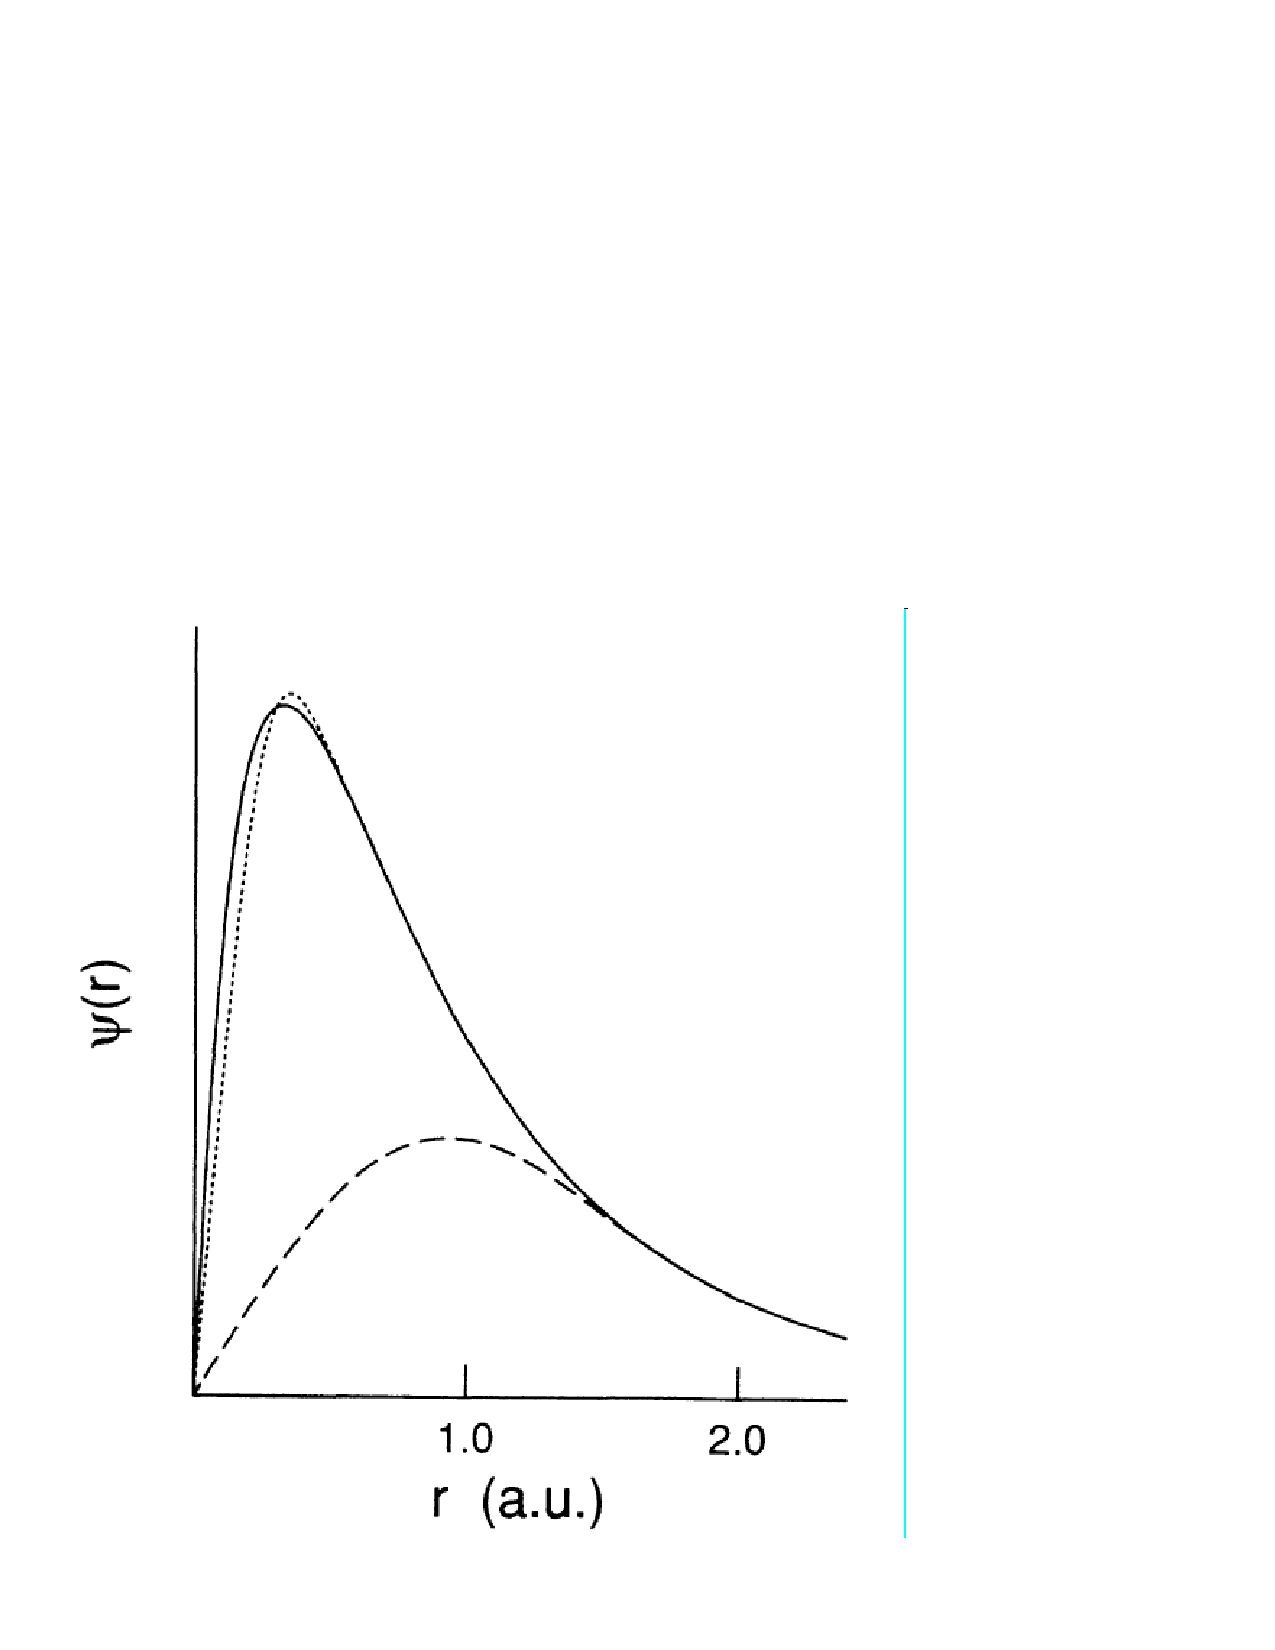
\includegraphics[height=1.35in,width=1.40in,viewport=30 55 415 500,clip]{Norm-US-wave.pdf}
\caption{\small \textrm{Oxygen 2} \textit{p} \textrm{radical wave function (solid), NC-pseudo-wave (dotted) and US-pseudo-wave (dashed).}}%(与文献\cite{EPJB33-47_2003}图1对比)
\label{Norm-US-wave}
\end{figure}

根据\textrm{Vanderbilt}的建议,对$1s$、$2p$、$3d$这种径向不包含节点的价电子波函数,构造赝波函数时选择平滑的函数,不再保持模守恒约束条件,只保留赝波函数与真实波函数在截断半径$r_c$以内的电荷密度差\footnote{模守恒约束下,\textrm{Schr\"odinger~}方程的求解是标准本征值问题;放弃模守恒条件,引入电荷密度差,\textrm{Schr\"odinger}方程D的求解变成广义本征值问题。}
\begin{equation}
	Q_{nm}(\vec r)=\varphi_n^{\ast}(\vec r)\varphi_m(\vec r)-\tilde\varphi_n^{\ast}(\vec r)\tilde\varphi_m(\vec r)
  \label{eq:uspp_4}
\end{equation}
策略上,这是通过增加少量的电荷密度差计算为代价(以保持赝势的可移植性),换取基函数规模的大大缩少。图\ref{Norm-US-wave}给出了\textrm{O}的2~\textit{p}~轨道的径向波函数在不同势函数下的形式,可以预见,超软赝势下的需要的平面波基函数数目最少。

超软赝势方法的实现步骤:
\begin{enumerate}
	\item 在构造平缓的赝波函数$|\phi_{lmj}(\vec r)\rangle$和局域势函数$V^L(\vec r)$的基础上,定义辅助函数$|\chi(\vec r)\rangle$
\begin{equation}
	|\chi_{lmj}(\vec r)\rangle=\bigg[\varepsilon_{lj}-\dfrac12\nabla^2-V^L(\vec r)\bigg]|\phi_{lmj}(\vec r)\rangle
  \label{eq:uspp_1}
\end{equation}
	\item 构造矩阵$\mathrm{D}$,其矩阵元$D_{ij}=\langle\phi_i|\chi_j\rangle$和局域投影函数$|\beta_i\rangle$
\begin{equation}
	|\beta_i\rangle=\sum_j(\mathbf{D}^{-1})_{ji}|\chi_{j}\rangle
  \label{eq:uspp_2}
\end{equation}
	\item 与模守恒赝势类似,将赝势的非局域部分用$\mathbf{D}$和$\beta_i$表示
\begin{equation}
	V_{NL}=\dfrac{|\chi_i\rangle\langle\chi_i|}{\langle\chi_i|\phi_i\rangle}=\sum_{i,j}\mathbf{D}_{ij}|\beta_i\rangle\langle\beta_j|
  \label{eq:uspp_3}
\end{equation}
\end{enumerate}
根据DFT的总能计算表达式
	\begin{equation} 
		\begin{aligned}
			E_{\mathrm{total}}=&\sum_j^{\mathrm{occ}}\langle\phi_{lmj}|\bigg[-\dfrac12\nabla^2+V_{\mathrm{local}}^{\mathrm{ion}}+\sum_{s,s^{\prime}}\mathbf{D}_{s,s^{\prime}}^{\mathrm{ion}}|\beta_s\rangle\langle\beta_{s^{\prime}}|\bigg]|\phi_{lmj}\rangle\\
			&+E_{H}[\rho_v]+E_{N-N}+E_{XC}[\rho_v]
		\end{aligned}
  \label{eq:uspp_5}
	\end{equation}
其中$\rho_v(\vec r)=\sum\limits_j^{\mathrm{occ}}\phi_{lmj}^{\ast}(\vec r)\phi_{lmj}(\vec r)+\sum\limits_{s,s^{\prime}}\sum\limits_j^{\mathrm{occ}}\langle\phi_{lmj}|\beta_{s^{\prime}}\rangle\langle\beta_s|\phi_{lmj}\rangle Q_{s,s^{\prime}}(\vec r)$
	$$V_{\mathrm{local}}^{\mathrm{ion}}=V_{local}-V_{\mathrm H}-V_{XC}$$
	\begin{equation}
		\mathbf{D}_{s,s^{\prime}}^{\mathrm{ion}}=\mathbf{D}_{s,s^{\prime}}-\int\mathrm{d}\vec r\big[V_{\mathrm{H}}(\vec r)+V_{\mathrm{XC}}(\vec r)\big]Q_{s,s^{\prime}}(r)
		\label{eq:uspp_6}
	\end{equation}
根据文献\inlinecite{PRB47-10142_1993}, $\mathbf{D}_{s,s^{\prime}}$称为超软赝势的强度指数(\textrm{strength parameter}),$\mathbf{D}_{s,s^{\prime}}^{\mathrm{ion}}$是其去屏蔽后的形式(有时也记为$\mathbf{D}_{s,s^{\prime}}^0$)。
可以得到广义本征值方程
\begin{equation}
	\bigg[-\dfrac12\nabla^2+V_{\mathrm{local}}+V_{NL}^{\mathrm{US}}-\varepsilon_i\bigg(\mathbf{1}+\sum_{s,s^{\prime}}Q_{s,s^{\prime}}|\beta_s\rangle\langle\beta_{s^{\prime}}|\bigg)\bigg]|\phi_{lmi}\rangle=0
	\label{eq:uspp_7}
\end{equation}

\subsubsection{线性缀加平面波(Linear Augmented Plane Wave, LAPW)方法}
%\subsubsection{APW与LAPW}
针对周期体系中不同区域势能与波函数的差别,Slater提出MT球近似,并建议将波函数分区域表示方法\cite{PR51-846_1937,PR91-528_1953},这也是缀加平面波(APW)方法的起源。如图\ref{Muffin_tin_0}所示,%后来Slater又对APW方法进行“简化”\cite{}%,但实际上原始的APW思想更直接。
\begin{figure}[h!]
\centering
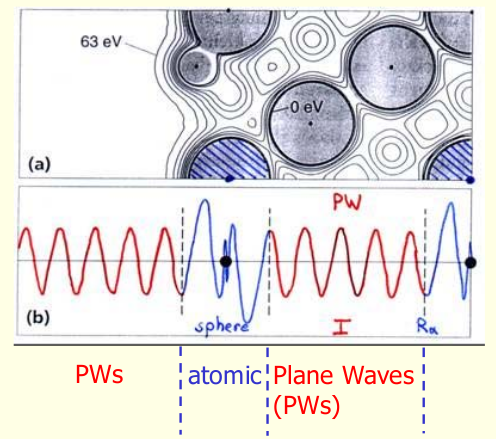
\includegraphics[height=1.30in,width=1.45in,viewport=1 20 485 435,clip]{APW.png}
\caption{\small \textrm{Partitioning of the unit cell into atomic spheres and an interstitial region.}}%(与文献\cite{EPJB33-47_2003}图1对比)
\label{Muffin_tin_0}
\end{figure}

在MT球之间的区域,波函数可用平面波表示
\begin{equation}
	\varphi(\vec k_i,\vec r)=\exp\mathrm{i}\vec k_i\vec r=\exp\mathrm{i}\vec k_i\cdot(\vec r_s+\vec r)
  \label{eq:solid-111}
\end{equation}
每个MT球内,%势能具有球对称性$V(r)$,MT球内的基
波函数则用类似原子波函数表示
\begin{equation}
  \varphi(\vec k_i,\vec r)=\sum_{l=0}^{\infty}\sum_{m=-l}^lA_{lm}(\vec k_i)u_l(|\vec r-\vec r_s|)Y_{lm}\widehat{(\vec r-\vec r_s)}
  \label{eq:solid-109}
\end{equation}
这里$Y_{lm}$是球谐函数;$\vec r_s$是第$s$个MT球心位置,$u_l(\vec r)$是MT球内的径向函数,和原子径向波函数类似,是方程
\begin{equation}
  -\frac1{r^2}\frac d{dr}\left(r^2\frac{du_l}{dr}\right)+\left[\frac{l(l+1)}{r^2}+V(r)\right]u_l=E_l^{\prime}u_l
  \label{eq:solid-110}
\end{equation}
的解;$A_{lm}$是待定系数,它的作用是使得两个区域的函数在MT球面上保持连续,因此$A_{lm}$也是倒空间矢量$\vec k_i$的函数,并有$\vec k_i=\vec k+\vec G_i$,$\vec G_i$倒格矢。为确定系数$A_{lm}$的值,将平面波用球谐函数展开,
\begin{equation}
	\exp(\mathrm{i}\vec k_i\cdot\vec r)=4\pi\sum_{l=0}^{\infty}\sum_{m=-l}^l\mathrm{i}^lj_l(|\vec k_i|r)Y_{lm}^{\ast}(\hat{\vec k}_i)Y_{lm}(\hat{\vec r})
  \label{eq:solid-112}
\end{equation}
这里$j_l(|\vec k_i|r)$是第$l$阶球Bessel函数;$\hat{\vec k}_i$和$\hat{\vec r}$是矢量$\vec k$和$\vec r$与$z$轴的夹角对应球坐标角度部分$\theta$和$\phi$。由函数在球面$R_{MT}^s$上连续条件,%要求式\eqref{eq:solid-109}和\eqref{eq:solid-111}在球面上数值相等,由此
得到系数$A_{lm}(\vec k_i)$:
$$A_{lm}(\vec k_i)=4\pi e^{\mathrm{i}\vec k_i\cdot\vec r_s}\mathrm{i}^lY_{lm}(\hat{\vec k}_i)j_l(|\vec k_i|R_{MT}^s)/u_l(E,R_{MT}^s)$$
式\eqref{eq:solid-110}中$E_l^{\prime}$是确定径向函数$u_l(r)$的边条件。所以APW的基组可以表示为:
\begin{equation}
  \begin{split}
    \varphi&(\vec k_i,\vec r)\\
    &=\left\{\begin{aligned}
	    &e^{\mathrm{i}\vec k_i\cdot\vec r_s}e^{\mathrm{i}\vec k_i\cdot\vec r},&|\vec r|>R_{MT}^s\\
	    &4\pi e^{\mathrm{i}\vec k_i\cdot\vec r_s}\sum_{lm}\mathrm{i}^lj_l(|\vec k_i|R_{MT}^s)Y_{lm}^{\ast}(\hat{\vec k}_i)Y_{lm}(\hat{\vec r})\dfrac{u_l(r,E^{\prime})}{u_l(R_{MT}^s,E^{\prime})},\quad&|\vec r|\leqslant R_{MT}^s
    \end{aligned} \right.
  \end{split}
  \label{eq:solid-113}
\end{equation}
不难看出,APW方法对波函数没有赝化处理,是一种高精度的方法,但APW方法构造的函数对能量$E_l^{\prime}$有依赖,无法作为有效的线性化方法应用。

%对于基函数在MT球面不连续的情形,用Schlosser和Marcus的能量变分表达式\cite{PR131-2529_1963},
%\begin{equation}
%  \begin{split}
%    E\int_{\mathrm{I+II}}\Psi^{\ast}\Psi dV=&\int_{\mathrm{I+II}}\Psi^{\ast}\mathbf H\Psi dV+\frac12\int_S\left[(\Psi_{\mathrm{II}}-\Psi_{\mathrm I})\frac{\partial}{\partial\rho}\Psi_{\mathrm {II}}^{\ast}+\frac{\partial}{\partial\rho}\Psi_{\mathrm I}^{\ast}\right.\\
%    &-(\Psi_{\mathrm {II}}^{\ast}+\Psi_{\mathrm I}^{\ast})\left.\left(\frac{\partial}{\partial\rho}\Psi_{\mathrm{II}}-\frac{\partial}{\partial\rho}\Psi_{\mathrm I}\right)\right]dS
%  \end{split}
%  \label{eq:solid-114}
%\end{equation}
%这里I和II分别表示MT球的内(I)外(II)两部分。上式中的前两个积分项表示对整个WS原胞的积分,第三个积分项是对MT球的球面S的积分。$\partial/\partial\rho$沿球面正方向对区域I的偏导。采用连续基函数,则\eqref{eq:solid-114}可以简化为:
%\begin{equation}
%  \begin{split}
%    E\int_{\mathrm{I+II}}\Psi^{\ast}\Psi dV=&\int_{\mathrm{I+II}}\Psi^{\ast}\mathbf H\Psi dV\\
%    &-\frac12\int_S(\Psi_{\mathrm {II}}^{\ast}+\Psi_{\mathrm I}^{\ast})\left(\frac{\partial}{\partial\rho}\Psi_{\mathrm{II}}-\frac{\partial}{\partial\rho}\Psi_{\mathrm I}\right)dS
%  \end{split}
%  \label{eq:solid-115}
%\end{equation}
%这里的球面积分是考虑波函数$\Psi$在MT球面上导数不连续。
%因为APW基函数径向部分与能量参数$E_l$有关,因此矩阵元与$E_l$有关。为了获得能量本征值$E_l$,必须求解$\vec k$-空间中每个点的能量$E_l$高阶行列式,该过程非常麻烦。
为了解除APW函数对能量$E_l$的相关,人们提出了多种线性化的实现方案\cite{PRB2-3098_1970,PRB2-290_1970,JPF9-661_1979,PRB19-6094_1979}。线性化缀加平面波(linearized augmented plane-wave, LAPW)方法是将径向波函数在给定能量值$E_{l0}$附近作Taylor展开到一阶\cite{PRB12-3060_1975},LAPW方法的基函数为:
\begin{equation}
  \varphi(\vec k_j,\vec r)=\left\{
  \begin{aligned}
	  &\Omega_0^{-1/2}\exp(\mathrm{i}\vec k_j\cdot\vec r),&r>R_{MT}^s\\
    &\sum_{lm}[A_{lm}u_l(E_l,r)+B_{lm}\dot u_l(E_l,r)]Y_{lm}(\hat{\vec r}),\quad&r\leqslant R_{MT}^s
  \end{aligned}\right.
  \label{eq:LAPW-basis}
\end{equation}
这里$R_{MT}^s$是MT球半径;$\vec k_j=\vec k+\vec G_j$,$\vec k$是不可约Brillouin区中的波矢;$\vec G_j$是倒空间格矢;$u_l(E_l,r)$是满足能量为$E_l$的径向Schr\"odinger方程的解波函数,不同的角动量$l$可指定不同的能量参数;$\dot u_l(E_l,r)$是解波函数对能量$E_l$的一阶导数;$Y_{lm}$是球谐函数;$\Omega_0$是WS原胞体积。APW与LAPW方法径向部分h函数在球面上附近衔接如图\ref{Muffin_tin}所示。
\begin{figure}[h!]
\centering
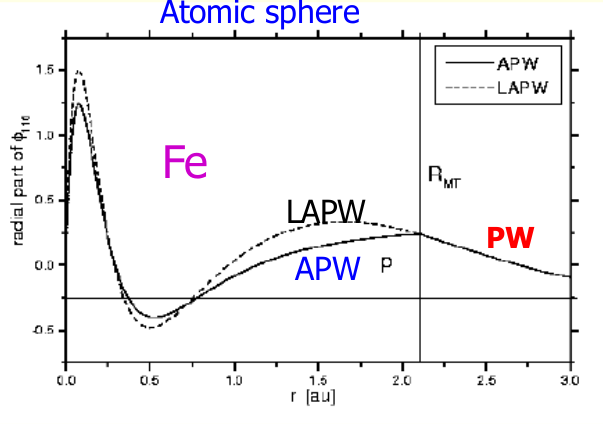
\includegraphics[height=1.30in,width=1.98in,viewport=1 20 585 435,clip]{WIEN2k-LAPW.png}
\caption{\small \textrm{Partitioning of the unit cell into atomic spheres(I) and an interstitial region(II)}}%(与文献\cite{EPJB33-47_2003}图1对比)
\label{Muffin_tin}
\end{figure}
显然LAPW方法的径向函数在球面上连续到一阶,比APW方法更平滑。另一方面,径向波函数线性化引入的误差,对势能的影响很小,因此能量参数的选择,对LAPW方法的基函数构造的Hamiltonian和重叠矩阵基本不会发生影响。这就是LAPW方法中能量参数$E_l$的取值范围可以比较大的原因。%Koelling和Arbman将LAPW方法应用于Cu的计算\cite{JPF5-2041_1975}。Smr\v cka提出了二次APW方法\cite{Smrcka}。
%与APW不同,这里$E_l$是指定范围内的能量参数,而非变量,

为了提高LAPW方法的线性化程度(即提高基组的变分自由度),在同一能量范围处理半芯态(接近价态的能量较高的芯态)和价态,可采用外加基函数(与$\vec k$无关)方案,这部分外加基函数称为局域轨道(local orbitals, LO)\cite{PRB43-6388_1991,Singh}。由此构造的基函数包含两个指定能量的径向波函数和其中一个能量导数,这样的基函数即LAPW-LO:
\begin{equation}
  \phi_{lm}^{LO}(\vec r)=[A_{lm}u_l(E_{1,l},r)+B_{lm}\dot u_l(E_{1,l},r)+C_{lm}u_l(E_{2,l},r)]Y_{lm}(\hat{\vec r})
  \label{eq:LAPW-LO}
\end{equation}
根据条件$\phi_{lm}^{LO}$在MT球面上数值为零且保持一阶导数连续,并要求$\phi_{lm}^{LO}$在MT球内归一化,可以确定系数$A_{lm}$,$B_{lm}$,$C_{lm}$。

%Sj\"ostedt等\cite{SSC114-15_2000}的计算表明,在标准LAPW方法中,将平面波展开使之在MT球面上与球内函数数值和一阶导数连续,这并非是实现Slater型APW方法最有效的线性化方法。采用指定能量参数$E_l$的APW形式的径向波函数[式\eqref{eq:APW-basis}],外加APW型局域轨道(local orbit, lo)扩展基函数,是更有效的方案,称为APW+lo。
%\begin{equation}
%  \varphi_{\vec k_i,\vec r}=\sum_{lm}[A_{lm}(\vec k_i)u_l(E_l,r)]Y_{lm}(\hat{\vec r})
%  \label{eq:APW-basis}
%\end{equation}
%\begin{equation}
%  \phi_{lm}^{lo}=[A_{lm}u_l(E_{1,l})+B_{lm}\dot u_l(E_{1,l})]Y_{lm}(\hat{\vec r})
%  \label{eq:APW-lo}
%\end{equation}
%APW+lo基函数式\eqref{eq:APW-lo}形式上与标准LAPW式\eqref{eq:LAPW-basis}形式非常相似,但这里系数$A_{lm}$和$B_{lm}$与$\vec k$无关,是根据式\eqref{eq:APW-lo}在MT球边界上数值为零并且在MT球内归一化确定。这样构造的APW+lo基函数,总的波函数在MT球面上平滑且一阶可导的,但是根据式\eqref{eq:solid-115},在MT球面上有动能部分对Hamiltonian的贡献。为收敛到相同的结果,采用APW+lo基组比起标准LAPW基组小得多\cite{PRB64-195134_2001}。因此选择APW+lo基组比标准LAPW基组的计算效率要高。

%WIEN2K程序包建议\cite{CPC59-399_1990,WIEN2K-UG_2001,CPC147-71_2002}一般平面波基函数收敛缓慢的轨道(比如过渡金属的3d态波函数)或MT球半径特别小的体系用APW+lo基组展开,其余价电子轨道用LAPW基组展开,此外对必要的半芯层可以用LO基组展开。用这样的方式可以同时考虑价态和半芯态。

%\subsubsection{FP-LAPW的总能计算}
%根据\textrm{APW}方法的基本思想,原子的芯电子的运动限于\textrm{MT}球内,价电子的运动范围遍及\textrm{MT}球区和间隙区。材料的物理和化学性质主要取决于体系的价电子状态,\textrm{WIEN2k}程序处理价电子时,对应的基函数在空间的不同位置采用不同的表示。
%
%所谓全势(\textrm{Full-potential})方法的思想,简言之,就是无论价电子在\textrm{MT}球区,还是在间隙区,感受到的都是包括芯层电子在内的其他电子的排斥势和各格点原子核的吸引势。原则上,对于周期性体系,已知体系的电荷密度分布,由\textrm{Poisson}方程,可以直接求得体系的\textrm{Coulomb}势。众所周知,由于靠近原子核的区域,电荷密度(及相应的\textrm{Coulomb}势)变化剧烈,因此直接的\textrm{Fourier}级数展开不易收敛。为了克服这一困难,\textrm{Weinert}\cite{JMP22-2433_1981}注意到间隙区的电子\textrm{Coulomb}相互作用只和间隙区的电荷密度及\textrm{MT}球区的电荷多极矩(\textrm{multipole moments})有关。它的基本思想是利用电荷多极矩和球形边界\textrm{Dirichlet}边值问题求解\textrm{MT}球内的\textrm{Coulomb}势分布,进而得到间隙区\textrm{Coulomb}势的分布。
%
%注意到\textrm{MT}球内电荷对间隙区势能的贡献\cite{Jackson}:
%\begin{equation}
%	V(r)=\sum_{l=0}^{\infty}\sum_{m=-l}^{l}\dfrac{4\pi}{2l+1}q_{lm}\dfrac{Y_{lm}(\hat r)}{r^{l+1}}
%	\label{eq_V-multi-mom}
%\end{equation}
%这里,$q_{lm}$是\textrm{MT}球内的电荷多极矩。
%%\begin{equation}
%%	\rho_I(\vec r)=\sum_{\vec K}\rho_I(\vec K)\mathrm{e}^{\mathrm{i}\vec K\cdot\vec r}
%%	\label{eq_rho_i_four}
%%\end{equation}
%
%在实际计算中,\textrm{MT}区球内的电荷多极矩$q_{lm}$由下式给出:
%\begin{equation}
%	q_{lm}=\int_{S}Y_{lm}^{\ast}(\hat r)r^l\rho(r)\mathrm{d}^3r
%	\label{eq_multi-mom}
%\end{equation}
%因此有可能重构\textrm{MT}球区的电荷密度分布,使它既有与实际电荷密度分布相同的电荷多极矩,又能有较好的\textrm{Fourier}收敛行为。
%\begin{equation}
%	\rho(\vec r)\rightarrow\tilde\rho(\vec r)=\rho_I(\vec r)\theta(\vec r\in I)+\sum_{spheres}\tilde\rho_i(\vec r)\theta(\vec r\in S_i)
%	\label{eq_pseudo-rho}
%\end{equation}
%间隙区电荷密度$\rho_I(\vec r)$变化平缓,可用方便地作\textrm{Fourier}级数展开:
%\begin{equation}
%	\rho_I(\vec r)=\sum_{\vec K}\rho_I(\vec K)\mathrm{e}^{\mathrm{i}\vec K\cdot\vec r}
%	\label{eq_rho_i_four}
%\end{equation}
%
%如果将间隙区的电荷密度延伸到\textrm{MT}球内,于是体系的电荷密度表示为:
%\begin{equation}
%	\rho(\vec r)=\rho_I(\vec r)+\sum_{spheres}\big[\rho_i(\vec r)-\rho_I(\vec r)\big]\theta(\vec r\in S_i) 
%	\label{eq_rho_rean}
%\end{equation}
%此时$\rho_I(\vec r)$可在整个空间作\textrm{Fourier}展开。其中延伸到\textrm{MT}球内(球心位置记作$\xi_i$)的间隙区电荷密度表示为:
%\begin{equation}
%	\rho_I(\vec r)=\sum_{\vec K}\rho_I(\vec K)\mathrm{e}^{\mathrm{i}\vec K\cdot\vec\xi_i}\mathrm{e}^{\mathrm{i}\vec K\cdot\vec r_i} 
%	\label{eq_rho_i_four_i}
%\end{equation}
%这里$\vec r_i=\vec r-\xi_i$。
%
%如果已知\textrm{MT}球内的真实电荷密度分布,第$i$个\textrm{MT}球内多极矩记作$q_{lm}^i$。
%%\begin{equation}
%%	q_{lm}^{Ii}=\biggl\{
%%	\begin{aligned}
%%		&\dfrac{\sqrt{4\pi}}3R_i^3\rho_I(K=0)\delta_{l0}\quadd \\
%%		&4\pi\mathrm{i}^l\sum_{\vec K\neq 0}\rho_I(\vec K)\dfrac{R_i^{l+3}j_{l+1}(\vec K\cdot\vec R)}{KR_i}\mathrm{e}^{\mathrm{i}\vec K\cdot\xi_i}Y_{lm}^{\ast}(\hat K)
%%	\end{aligned}\biggr.
%%	\label{eq_multi_PW}
%%\end{equation}
%延伸到球内的间隙区电荷对球内多极矩的贡献即为:
%\begin{equation}
%	q_{lm}^{Ii}=\dfrac{\sqrt{4\pi}}3R_i^3\rho_I(K=0)\delta_{l0}+4\pi\mathrm{i}^l\sum_{\vec K\neq 0}\rho_I(\vec K)\dfrac{R_i^{l+3}j_{l+1}(\vec K\cdot\vec R)}{KR_i}\mathrm{e}^{\mathrm{i}\vec K\cdot\xi_i}Y_{lm}^{\ast}(\hat K)
%	\label{eq_multi_PW}
%\end{equation}
%这里利用了平面波在球心$\xi_i$处的球谐函数展开关系:
%\begin{equation}
%	\mathrm{e}^{\mathrm{i}\vec K\cdot \vec r}=\sum_{lm}4\pi\mathrm{i}^lj_l(\vec K\cdot\vec r)Y_{lm}^{\ast}(\hat{\vec K})Y_{lm}(\hat{\vec r})
%	\label{eq_PW_Bessel}
%\end{equation}
%和积分表达式:
%\begin{equation}
%	\int_0^R r^{l+2}j_l(\vec K\cdot\vec r)\mathrm{d}r=\left\{
%	\begin{aligned}
%		&\dfrac{R^3}3\delta_{l,0}\quad &\vec K=0\\ 
%		&\dfrac{R^{l+3}j_{l+1}(\vec K\cdot\vec R)}{KR} &\vec K\neq 0
%	\end{aligned}\right.
%	\label{eq_int_r_j}
%\end{equation}
%
%因此,重构方程\eqref{eq_rho_rean}在\textrm{MT}球内的电荷密度分布,其多极矩满足:
%\begin{equation}
%	\tilde q_{lm}^i=q_{lm}^i-q_{lm}^{Ii}
%	\label{eq_psmult}
%\end{equation}
%根据文献\inlinecite{JMP22-2433_1981},可以得到重构的\textrm{MT}球内的赝电荷密度的\textrm{Fourier}展开系数为:
%\begin{equation}
%	\tilde\rho_s(\vec K)=\dfrac{4\pi}{\Omega}\sum_{lm,i}\dfrac{(-\mathrm{i})^l(2l+2n+3)!!}{(2l+1)!!}\times\dfrac{j_{l+n+1}(\vec K\cdot\vec R_i)}{(KR_i)^{n+1}}\tilde q_{lm}^i\mathrm{e}^{-\mathrm{i}\vec K\cdot\vec\xi_i}Y_{lm}(\hat K)
%	\label{eq_psrho}
%\end{equation}
%这里$n$是整数。$\tilde\rho_s(\vec K)$可以视为$n$的函数,文献\inlinecite{JMP22-2433_1981}讨论了对于不同的$l$和$(\vec K\cdot\vec R_i)_{max}$,优化$n$值得到最佳收敛的$\tilde\rho_s(\vec K)$的情况。一般取$n=\big[\dfrac12(\vec K\cdot\vec R_i)_{max}\big]$,\textrm{WIEN2k}程序中取$n=9$。
%
%当$\vec K=0$,有
%$$\tilde\rho_s(\vec K=0)=\dfrac{\sqrt{4\pi}}{\Omega}\sum\limits_i\tilde q_{00}^i$$
%因此,用于计算间隙区\textrm{Coulomb}势的赝电荷密度(较平缓)可写成\textrm{Fourier}展开形式:
%\begin{equation}
%	\tilde\rho(\vec r)=\sum_{\vec K}\big[\rho_I(\vec K)+\tilde\rho_s(\vec K)\big]\mathrm{e}^{\mathrm{i}\vec K\cdot\vec r}
%	\label{eq_psrho_four}
%\end{equation}
%求解\textrm{Poisson}方程,间隙区的\textrm{Coulomb}势表达式为:
%\begin{equation}
%	V_I(\vec r)=\sum_{\vec K}\dfrac{4\pi}{K^2}\big[\rho_I(\vec K)+\tilde\rho_s(\vec K)\big]\mathrm{e}^{\mathrm{i}\vec K\cdot\vec r}
%	\label{eq_Vcou_I}
%\end{equation}
%与此同时,根据文献\inlinecite{JMP22-2433_1981},已知球面上的\textrm{Coulomb}势,根据\textrm{Dirichlet}的球形边值问题\cite{Jackson},可知\textrm{MT}球内的\textrm{Coulomb}势的表达式\cite{Singh,Nemoshkalenko-Antonov}为:
%\begin{equation}
%	\begin{aligned}
%		V_s(\vec r)=&\sum_{lm}Y_{lm}(\hat r)\left[\dfrac{4\pi}{2l+1}\left\{\dfrac1{r^{l+1}}\int_0^r\mathrm{d}r^{\prime}(r^{\prime})^{l+2}\rho_{lm}(r^{\prime})+r^l\int_r^{R_i}\mathrm{d}r^{\prime}(r^{\prime})^{1-l}\rho_{lm}(r^{\prime})\right\}\right.\\
%		&\left.+\left(\dfrac r{R_i}\right)^l4\pi\mathrm{i}^l\sum_{\vec K\neq0}\dfrac{4\pi}{K^2}\tilde\rho_s(\vec K)Y_{lm}^{\ast}(\vec K)\dfrac{\vec K\cdot\vec R_ij_{l-1}(\vec K\cdot\vec R_i)}{2l+1}\right]
%	\end{aligned}
%	\label{eq_Vcou_s}
%\end{equation}
%%球面$R_i$上的\textrm{Coulomb}势可以表达为
%%\begin{equation}
%%	V_{l=0}(R_i)=4\pi\sum_{\vec K\neq0}\dfrac{\vec K\cdot\vec R_i\tilde\rho_s(\vec K)}{K^2}Y_{00}^{\ast}(\vec K)j_0(\vec K\cdot\vec R_i)
%%	\label{eq_Vcou_S}
%%\end{equation}
%
%注意到由于\textrm{MT}球的存在,倒空间不连续,即
%\begin{equation}
%	V_I(\vec r)=\left\{\sum_{\vec K}\dfrac{4\pi}{K^2}\bigg[\tilde\rho_I(\vec K)+\tilde\rho_s(\vec K)\bigg]\mathrm{e}^{\mathrm{i}\vec K\cdot\vec r}\right\}\theta(r)\qquad(r\in \mathrm{Interstitial})
%	\label{eq_Vcou_I_theta}
%\end{equation}
%%由于间隙区的势能变化平缓,基函数是平面波,因此可以\textbf{重新定义能量零点,先将$V_C(\vec K=0)$置为零。}
%倒空间中的势能表示为:
%\begin{equation}
%	V_I(\vec K)=\left\{
%	\begin{aligned}
%		&\mathrm{divergence} \qquad &\vec K=0 \\
%		\dfrac{(4\pi)^2}{K^3}\bigg[\rho_I(\vec K)+&\tilde\rho_s(\vec K)\bigg]\sum_i\dfrac{R_i^2j_1(\vec K\cdot\vec R_i)}{\Omega}\mathrm{e}^{-\mathrm{i}\vec K\cdot\vec\xi_i}\quad &\vec K\neq0
%	\end{aligned}\right.
%	\label{eq_Vcou_KI_theta}
%\end{equation}
%显然,由于$\vec K=0$项的存在,使得间隙区的电子\textrm{Coulomb}势具有发散性。
%%在\textrm{MT}球内,按照原子\textrm{Coulomb}相互作用表达式可以参考文献\inlinecite{Singh,Nemoshkalenko-Antonov}。
%
%综上所述,\textrm{LAPW}方法中在\textrm{MT}球内和间隙区分别采用\eqref{eq_Vcou_s}和\eqref{eq_Vcou_I_theta}的势函数形式,实现全势(\textrm{full potential})\cite{PRB26-4571_1982,PRB33-823_1986}计算。
%%一般是在每个\textrm{MT}球内,势函数用球谐函数(或者是满足晶体对称性的球谐函数)展开,MT球外的势函数用\textrm{Fourier}级数展开\cite{PRB13-5362_1976}
%
%引入\textrm{Madelung}势,完成总能量的计算过程\cite{JMP22-2433_1981}:
%\begin{equation}
%	\begin{aligned}
%	E_T[\rho]=&T_s[\rho]+U[\rho]+E_{xc}[\rho]\\
%	=&T_s[\rho]+\dfrac12\biggl[\int\dfrac{\rho(\vec r)\rho(\vec r^{\prime}){}}{|\vec r-\vec r^{\prime}|}\mathrm{d}\vec r\mathrm{d}\vec r^{\prime}-2\sum_{\alpha}Z_{\alpha}\int\dfrac{\rho(\vec r)\mathrm{d}\vec r}{|\vec r-\vec R_{\alpha}|}+\sideset{}{^\prime}\sum_{\alpha,\beta}\dfrac{Z_{\alpha}Z_{\beta}}{|\vec R_{\alpha}-\vec R_{\beta}|}\biggr]\\
%	&+E_{xc}[\rho]\\
%	=&T_s[\rho]+\dfrac{N}2\bigg[\int_{\Omega}\rho(\vec r)V_c(\vec r)\mathrm{d}\vec r-\sum_{\nu}Z_{\nu}V_M(\vec\gamma_{\nu})\biggr]+E_{xc}[\rho]
%	\end{aligned}
%	\label{eq_E_total}
%\end{equation}
%这里$V_c(\vec r)$是\textrm{Coulomb}势:
%\begin{equation}
%	V_c(\vec r)=\int\dfrac{\rho(\vec r^{\prime})}{|\vec r-\vec r^{\prime}|}\mathrm{d}\vec r^{\prime}-\sum_{\alpha}\dfrac{Z_{\alpha}}{|\vec r-\vec R_{\alpha}|}
%	\label{eq_Vcou_WIEN}
%\end{equation}
%$V_M(\vec\gamma_{\nu})$是\textrm{Madelung}势:
%\begin{equation}
%	V_M(\vec\gamma_{\nu})=\int\dfrac{\rho(\vec r)\mathrm{d}\vec r}{|\vec r-\vec\gamma_{\nu}|}-\sideset{}{^\prime}\sum_{\alpha}\dfrac{Z_{\alpha}}{|\vec R_{\alpha}-\vec\gamma_{\nu}|}
%	\label{eq_Vmadelung}
%\end{equation}
%即将离子相互作用、电子间相互作用和离子-电子相互作用分为电子感受的\textrm{Coulomb}势和原子核位置的\textrm{Madelung}势贡献。因此利用电子的\textrm{Coulomb}势与\textrm{Madelung}势在球心处的贡献的球形部分彼此抵消来排除奇点:
%
%球心位于$\vec\gamma_{\nu}$、半径为$R_{\nu}$的\textrm{MT}球球面上的势能平均值$S_0(R)$可由式\eqref{eq_Vcou_s}计算,因此除去球心核电荷以外所有电荷在MT球面上产生的势能平均为:
%\begin{equation}
%  S(R_{\nu})\equiv S_0(R_{\nu})+Z_{\nu}/R_{\nu}
%  \label{eq:solid-79}
%\end{equation}
%因此球心$\vec\gamma_{\nu}$处的\textrm{Madelung}势的球对称部分贡献为\cite{PRB26-4571_1982}:
%\begin{equation}
%  \begin{split}
%	  V_M(\vec\gamma_{\nu})&=\frac1{R_{\nu}}\big[R_{\nu}S_0(R_{\nu})+Z_{\nu}-Q_{\nu}\big]+\sqrt{4\pi}\int_0^{R_{\nu}}\mathrm{d}rr\rho_{00}(r)\\
%	   &=\frac1{R_{\nu}}\big[R_{\nu}S_0(R_{\nu})+Z_{\nu}-Q_{\nu}\big]+\bigg\langle\frac1r\rho(\vec r)\bigg\rangle_{\nu}
%  \end{split}
%   \label{eq:Madelung}
%\end{equation}
%其中$Q_{\nu}$表示\textrm{MT}球内的电子电荷之和。$\rho(\vec r)$是\textrm{MT}球内的电荷密度,可以用球谐函数表示为:
%\begin{equation}
%  \rho(\vec r_{\nu})=\sum_{lm}\rho_{lm}(r_{\nu})Y_{lm}(\hat r_{\nu})
%  \label{eq:solid-80}
%\end{equation}
%因此\textrm{MT}球内的总能量贡献为:
%\begin{equation}
%  \begin{split}
%	  E_T=\sum_i\varepsilon_i&-\frac12\int_{\Omega}\rho(\vec r)\big[V_c(\vec r)+\mu_{xc}(\vec r)\big]\mathrm{d}\vec r-\frac12\sum_{\nu}Z_{\nu}V_M(\vec\gamma_{\nu})+E_{xc}[\rho] \\
%   =\sum_i\varepsilon_i&-\frac12\left(\int_{\Omega}\rho(\vec r)V_c(\vec r)\mathrm{d}\vec r+\sum_{\nu}Z_{\nu}\bigg\langle\frac1r\rho(\vec r)\bigg\rangle_{\nu}\right)-\dfrac12\int_{\Omega}\rho(\vec r)\mu_{xc}(\vec r)\mathrm{d}\vec r\\
%   &-\frac12\sum_{\nu}\frac{Z_{\nu}}{R_{\nu}}\big[R_{\nu}S_0(R_{\nu})+Z_{\nu}-Q_{\nu}\big]+E_{xc}[\rho]
%  \end{split}
%  \label{eq:solid-81}
%\end{equation}
%这里$V_c(\vec r)=\displaystyle\int\dfrac{\rho(\vec r\,^\prime)}{|\vec r-\vec r\,^\prime|}\mathrm{d}\vec r\,^\prime-\sum\limits_{\alpha}\dfrac{Z_{\alpha}}{|\vec r-\vec R_{\alpha}|}$。总能量写成这样的形式,原子核位置的\textrm{Coulomb}势奇点可以排除。将势能和电荷密度在各原子核附近作球谐展开,在原子核附近,有
%\begin{equation}
%  \begin{split}
%	  &\int_{\Omega}\rho(\vec r)V_c(\vec r)\mathrm{d}\vec r+Z_{\nu}\sqrt{4\pi}\int_0^{R_{\nu}}\mathrm{d}rr^2\frac{\rho_{00}(r)}r\\
%	  =&\sqrt{4\pi}\int\mathrm{d}rr^2\rho_{00}(r)\left[V_{00}(r)Y_{00}(\hat r)+\frac{Z_{\nu}}r\right]+\sum_{lm>0}\int\mathrm{d}rr^2\rho_{lm}(r)V_{lm}(r)
%  \end{split}
%\end{equation}
%\textrm{Coulomb}势的奇点只出现在$V_{00}(r)$中,将$V_{00}(r)$写成核的点电荷势与源于电子的平滑势两部分之和,有
%$$V_{00}(r)=-\sqrt{4\pi}\frac{Z_{\nu}}r+\hat V_{00}(r)$$
%通过这样的方式,可以将总能量中的奇点排除,但同样单独\textrm{Coulomb}势和\textrm{Madelung}势每一项在原子核位置能量仍然是发散的。
%
%%如果采用标准的\textrm{LDA}近似,式\eqref{eq:solid-81}交换-相关能可以写成:
%%\begin{equation}
%%  E_{xc}[\rho]\approx\int_{\Omega}\rho(\vec r)\varepsilon_{xc}(\vec r)d\vec r
%%  \label{eq:solid-82}
%%\end{equation}
%基于\textrm{LAPW}方法的总能量计算,在空间中不同的区域采用不同的表示。%间隙区(\textrm{I})的电荷密度用平面波展开,有
%%$$\rho(\vec r)=\sum_{\vec G}\rho(\vec G)e^{i\vec G\cdot\vec r},\quad \vec r\in\mathrm{I}$$
%%在\textrm{MT}球内,电荷密度用球谐函数展开,在动量空间中的展开形式为:
%%$$\bar\rho_{lm}(r_{\nu})=4\pi i^l\sum_{\vec G}\rho(\vec G)e^{i\vec G\cdot\vec r_{\nu}}j_l(Gr_{\nu})Y_{lm}^{\ast}(\vec G)$$ 
%首先,将间隙区$V_C(\vec K=0)$置零,排除间隙区的\textrm{Coulomb}势$V_I(\vec K)$的奇点:
%\begin{equation}
%	\tilde V_I(\vec K)=\left\{
%	\begin{aligned}
%		&0 \qquad &\vec K=0 \\
%		\dfrac{(4\pi)^2}{K^3}\big[\rho_I(\vec K)+&\tilde\rho_s(\vec K)\big]\sum_i\dfrac{R_i^2j_1(\vec K\cdot\vec R_i)}{\Omega}\mathrm{e}^{\mathrm{i}\vec K\cdot(\vec r-\vec\xi_i)}\quad &\vec K\neq0
%	\end{aligned}\right.
%	\label{eq_Vcou_KI_theta_2}
%\end{equation}
%%在总能量计算中补偿这一平移。
%\textrm{MT}球内对总能量的贡献部分在正空间中按上述式\eqref{eq:solid-81}计算。
%
%因此\textrm{LAPW}方法的原胞内的晶体总能量可以写成:
%\begin{equation}
%  \begin{split}
%	  E=&\sum_i\varepsilon_i-\sum_{\vec K}\Omega\rho_I(\vec K)\tilde V_I^{\ast}(\vec K)-\frac12\sum_{\nu}\dfrac{Z_{\nu}}{R_{\nu}}[Z_{\nu}-Q_{\nu}+R_{\nu}S_0(R_{\nu})]\\
%    &-\sum_{\nu}\sum_{lm}\int_0^{R_{\nu}}\mathrm{d}rr^2\left[\rho_{lm}(r_{\nu})\left(\tilde V_{lm}^{\ast}(r_{\nu})+\dfrac{\sqrt{4\pi}}{2r_{\nu}}Z_{\nu}\delta_{l0}\right)-\bar\rho_{lm}(\vec r_{\nu})\bar V_{lm}^{\ast}(\vec r_{\nu})\right]
%  \end{split}
%  \label{eq:solid-83}
%\end{equation}
%这里$\tilde V(\vec r)$和$\bar V_{lm}(\vec r)$根据都按下式计算:
%$$\tilde V(\vec r)=\frac12V_c(\vec r)-\varepsilon_{xc}(\vec r)+\mu_{xc}(\vec r)$$

%\textrm{WIEN2k}程序中,\textbf{程序\textrm{lapw0}部分完成式\eqref{eq:solid-83}中除$\sum\limits_i\varepsilon_i$之外的所有各项的计算}。
%\subsection{LDA+U和GW近似}
%\subsubsection{GW近似}
%Landau的Fermi液体理论是研究群体激发和多体Fermi子体系物理性质的重要方法\cite{Landau}。Fermi液体的特征是准粒子分布$\varepsilon=\varepsilon(\vec k)$由体系总能量$E$对分布函数的变分,即
%\begin{equation}
%  \frac{\delta E}{\delta n(\vec k)}=\varepsilon(\vec k)
%  \label{eq:solid-219}
%\end{equation}
%关联函数$f(\vec k,\vec k^\prime)$由准粒子能量对整个$\vec k$空间粒子分布变分得到
%\begin{equation}
%  \frac{\delta\varepsilon(\vec k)}{\delta n(\vec k^\prime)}=\frac{\delta^2E}{\delta n(\vec k)\delta n(\vec k^\prime)}=f(\vec k,\vec k^\prime)
%  \label{eq:solid-220}
%\end{equation}
%考虑准粒子间相互作用,体系激发能记作
%\begin{equation}
%  W=\sum_{\vec k}\varepsilon(\vec k)\delta n(\vec k)+\frac12\sum_{\vec k}\sum_{\vec k^\prime}f(\vec k,\vec k^\prime)\delta n(\vec k)\delta(\veck^\prime)
%  \label{eq:solid-221}
%\end{equation}
%
%Green函数是研究Fermi液体的重要数学工具。对宏观体系,Green函数定义为\cite{Lifshitz}
%\begin{equation}
%  \tilde G(x,x^\prime)=-i\langle T\hat\Psi(x)\hat\Psi^{\ast}(x^\prime)\rangle
%  \label{eq:solid-222}
%\end{equation}
%这里$x$表示时间$t$和位置$\vec r$,$\langle\cdots\rangle$表示对体系基态求平均,$T$表示按时间先后乘积算符。$\hat\Psi$是Heisenberg算符,对式\eqref{eq:solid-222}进行Fourier变换,得到以$\vec r$,$E$为表象的Green函数$\tilde G(\vec r,\vec r\,^\prime;E)$是Dyson方程\cite{Lifshitz}
%\begin{equation}
%  (\nabla^2+E)\tilde G(\vec r,\vec r\,^\prime;E)-\int d\vec r^{\prime\prime}\Sigma(\vec r,\vec r^{\prime\prime};E)\tilde G(\vec r^{\prime\prime},\vec r\,^\prime;E)=\delta(\vec r-\vec r\,^\prime)
%  \label{eq:solid-223}
%\end{equation}
%的解。这里$\Sigma(\vec r,\vec r\,^\prime;E)$是描述交换和相关效应的质量或自能算符,这是个与能量有关的非定域的非-Hermitian算符,考虑到粒子与体系中其他粒子的相互作用。晶体中的质量具有平移对称性,
%\begin{equation}
%  \Sigma(\vec r+\vec a,\vec r+\vec a;E)=\Sigma(\vec r,\vec r\,^\prime;E),
%  \label{eq:solid:224}
%\end{equation}
%这里$\vec a$是晶体平移格矢。
%
%临近Green函数的极点,式\eqref{eq:solid-223}右面的$\delta$函数为0,所得积分-微分方程的本征值确定体系激发能谱\cite{Lifshitz,PR145-561_1966}
%\begin{equation}
%  -\delta^2\Phi_{\vec k}(\vec r,E)+\int d\vec r\,^\prime\Sigma(\vec r,\vec r\,^\prime;E)\Phi_{\vec k}(\vec r\,^\prime,E)=\varepsilon_{\vec k}\Phi_{\vec k}(\vec r,E) 
%  \label{eq:solid-225}
%\end{equation}
%这里函数$\Phi_{\vec k}(\vec r,E)$类似于周期场中的单电子Bloch波函数。对金属中的Fermi电子液体中用式\eqref{eq:solid-225}替代一般Schr\"odinger方程。与一般的Schr\"odinger方程不同,式\eqref{eq:solid-225}的能量本征值是复数,因为质量算符$\Sigma(\vec r,\vec r\,^\prime;E)$是复数。
%
%由式(\ref{eq:solid-223},\ref{eq:solid-225})得到Green函数
%\begin{equation}
%  \tilde G(\vec r,\vec r\,^\prime;E)=\sum_{\vec k}\frac{\Phi_{\vec k}(\vec r,E)\Phi_{\vec k}^{\ast}(\vec r\,^\prime,E)}{E-\varepsilon_{\vec k}(E)+i0\mathrm{sign}E}
%  \label{eq:solid-226}
%\end{equation}
%$\varepsilon_{\vec k}(E)$是体系中加入一个粒子引起的能量改变。如果将单个准粒子改变引起得能量变化$\varepsilon_{\vec k}(E)$定义为式\eqref{eq:solid-219}中的准粒子能量,对临近Fermi面的态,函数$\tilde G(\vec r,\vec r\,^\prime;E)$在$E=\varepsilon_{\vec k}(E)$有极值。因此Green函数极值确定了多Fermi子体系的元激发能谱。一般说,因为和其他粒子相互作用,准粒子能量为复数。复数能量使得体系激发态的寿命有限$(\tau\sim1/|\mathrm{Im}\varepsilon|)$\cite{Landau-Lifshitz}。能量宽度由$\mathrm{Im}\varepsilon$确定。
%
%%临近Fermi能级,$\mathrm{Im}\varepsilon_{\vec k}(E)\rightarrow0$,相应的$\mathrm{Im}\Sigma\rightarrow0$,于是解方程\eqref{eq:solid-225}得到$\mathrm{Re}\varepsilon_{\vec k}(E)$和实数形式的$\Sigma(\vec r,\vec r\,^\prime;E)$和$\epsilon_{\vec k}(E)$。
%
%根据Hohenberg-Kohn定理,本征值$\Sigma(\vec r,\vec r\,^\prime;E)$由体系基态确定,它也是电子密度的函数。Sham和Kohn建议可用局域电子密度近似表示$\Sigma(\vec r,\vec r\,^\prime;E)$\cite{PR145-561_1966}:
%\begin{equation}
%  \Sigma(\vec r,\vec r\,^\prime;E)=V_C(\vec r)\delta(\vec r-\vec r\,^\prime)+\Sigma_0(\vec r-\vec r\,^\prime;E-V_C(\vec r_0);\rho(\vec r_0))
%  \label{eq:solid-227}
%\end{equation}
%这里$\Sigma_0$是密度为$\rho$的无相互作用电子气的本征能量,$V_C(\vec r_0)$是位于$\vec r_0=(\vec r+\vec r\,^\prime)/2$的静电Coulomb势。此外式\eqref{eq:solid-227}已将能量$\Sigma$中的局域部分以Hartree势的形式分离出来,因此可以利用$\Sigma_0$的短程效应。
%
%对本征函数$\Phi_{\vec k}$作近似
%$$\Phi_{\vec k}(\vec r,E)=A(\vec k)\exp[i\vec p(\vec r)\vec r]$$
%并认为$A$和电子动量与$\vec r$无关,将式\eqref{eq:solid-225}称为类似Kohn-Sham方程的表达式\cite{JPC4-2064_1971},
%\begin{equation}
%  [-\nabla^2+V_C(\vec r)+\Sigma_{xc}(\rho(\vec r),E)]\Phi_{\vec k}(\vec r,E)=\varepsilon_{\vec k}(\vec r,E)
%  \label{eq:solid-228}
%\end{equation}
%若$E=\mu$,$\Sigma_{xc}(\rho(\vec r),\mu)\equiv\mu_{xc}(\rho(\vec r))$我们因此得到符合局域密度近似的DFT方程,两者的交换-相关势$\mu_{xc}$是相同的。因此对于低激发能,可以使用近似$\Sigma_{xc}(\rho(\vec r),E)\simeq\mu_{xc}$,此结果对应于忽略准粒子间的相互作用,即Landau函数$f(\vec k,\vec k^\prime)=0$。
%
%因此基于DFT的能带计算,如果充分考虑交换-相关效应,可以计算多电子体系的元激发能量。注意,采用单电子近似,要求能带比较宽,即中心位于不同格点的波函数有较大的重叠,电子间相互作用不是很强。
%
%Hedin和Lundqvist详细回顾了用Green函数技术解决电子相关的问题\cite{Hedin-Lundqvist}。在单粒子近似下的Green函数,准粒子与谱函数的峰联系在一起。如果峰足够尖锐,表明存在一个明确的准粒子能量,对一般的非均匀体系,准粒子能量和波函数可以通过解Dyson方程\eqref{eq:solid-225}求得。对于准粒子问题,核心问题是对自能算符$\Sigma(\vec r,\vec r\,^\prime;E)$的足够好的近似。常用的方法是GW近似\cite{PR139-A796_1965},自能用屏蔽相互作用$W$计算到最低阶。
%\begin{equation}
%  \Sigma(\vec r,\vec r\,^\prime;E)=\frac i{2\pi}\int_{-\infty}^{\infty}dE^\prime\tilde G(\vec r,\vec r\,^\prime;E+E^\prime)W(\vec r,\vec r\,^\prime;E^\prime)
%  \label{eq:solid-229}
%\end{equation}
%Green函数$\tilde G$由准粒子的波函数和能量表示,屏蔽Coulomb作用$W$
%\begin{equation}
%  W(\vec r,\vec r\,^\prime;E)=\frac1{\Omega}\int d^3r^{\prime\prime}\varepsilon^{-1}(\vec r,\vec r^{\prime\prime};E)V(\vec r^{\prime\prime}-\vec r\,^\prime)
%  \label{eq:solid-230}
%\end{equation}
%这里$V$是未屏蔽的Coulomb势,$\varepsilon^{-1}$是介电函数矩阵的逆阵,
%\begin{equation}
%  \varepsilon^{-1}(\vec r,\vec r\,^\prime;E)=\delta(\vec r-\vec r\,^\prime)+\int d^3r^{\prime\prime} V(\vec r\,^\prime-\vec r^{\prime\prime})P(\vec r^{\prime\prime},\vec r\,^\prime;E)
%  \label{eq:solid-231}
%\end{equation}
%这里$P$是完全响应函数,于是
%\begin{equation}
%  W(\vec r,\vec r\,^\prime;E)=V(\vec r-\vec r\,^\prime)+W_c(\vec r,\vec r\,^\prime;E)
%  \label{eq:solid-232}
%\end{equation}
%这里
%\begin{equation}
%  W_c(\vec r,\vec r;E)=\int d^3r_1d^3r_2V(\vec r\,^\prime-\vec r_1)P(\vec r_1,\vec r_2;E)V(\vec r_2-\vec r\,^\prime)
%  \label{eq:solid-233}
%\end{equation}
%Green函数可以写成谱表示
%\begin{equation}
%  G(\vec r,\vec r\,^\prime;E)=\int_{-\infty}^{\mu}dE^\prime\frac{A(\vec r,\vec r\,^\prime;E^\prime)}{E-E^\prime-i\delta}+\int_{\mu}^{\infty}dE^\prime\frac{A(\vec r,\vec r\,^\prime;E^\prime)}{E-E^\prime+i\delta}
%  \label{eq:solid-234}
%\end{equation}
%这里$A(\vec r,\vec r\,^\prime;E)=-\frac1{\pi}\mathrm{Im}G(\vec r,\vec r\,^\prime;E)\mathrm{sgn}(E-\mu)$
%
%实际计算中,取零阶Green函数,有
%\begin{equation}
%  A(\vec r,\vec r\,^\prime;E)=\sum_{kn}\psi_{kn}(\vec r)\psi_{kn}^{\ast}(\vec r\,^\prime)\delta(E-E_{kn})
%  \label{eq:solid-235}
%\end{equation}
%于是自能可以写成
%\begin{equation}
%  \Sigma(\vec r,\vec r\,^\prime;E)=\Sigma_x(\vec r,\vec r\,^\prime)+\Sigma_c(\vec r,\vec r\,^\prime;E)
%  \label{eq:solid-236}
%\end{equation}
%这里$\Sigma_x$是净的交换势,
%\begin{equation}
%  \Sigma_x(\vec r,\vec r\,^\prime)=-\sum_{kn}^{occ}\psi_{kn}(\vec r)\psi_{kn}^{\ast}(\vec r\,^\prime)V(\vec r-\vec r\,^\prime)
%  \label{eq:solid-254}
%\end{equation}
%$E_c$自能的相关部分,
%\begin{equation}
%  \begin{split}
%    \Sigma_c(\vec r,\vec r\,^\prime;E)=&\sum_{kn}^{occ}\psi_{kn}(\vec r)\psi_{kn}^{\ast}(\vec r\,^\prime)W_c^-(\vec r,\vec r\,^\prime;E-E_{kn})\\
%    &+\sum_{kn}^{occ}\psi_{kn}(\vec r)\psi_{\vec r}^{\ast}(\vec r\,^\prime)W_c^+(\vec r,\vec r\,^\prime;E-E_{kn})
%  \end{split}
%  \label{eq:solid-237}
%\end{equation}
%其中$W_c^{\pm}(\vec r,\vec r\,^\prime;E)=\dfrac i{2\pi}\displaystyle\int_{-\infty}^{+\infty}dE^\prime\frac{W_c(\vec r,\vec r\,^\prime;E^\prime)}{E+E^\prime\pm i\delta}$。于是$\Sigma(\vec r,\vec r\,^\prime;E)$可以记作\cite{JPCM9-767_1997},
%\begin{displaymath}
%  \Sigma(\vec r,\vec r\,^\prime;E)=-\sum_{kn}\psi_{kn}(\vec r)\psi_{kn}^{\ast}(\vec r\,^\prime)W_0(\vec r,\vec r\,^\prime;E-E_{kn})
%\end{displaymath}
%其中
%\begin{displaymath}
%  \begin{split}
%    W_0(\vec r,\vec r\,^\prime;E-E_{kn})\equiv&[V(\vec r-\vec r\,^\prime)-W_c^-(\vec r,\vec r\,^\prime;E-E_{kn})]\theta(\mu-E_{kn})\\
%    &-W_c^+(\vec r,\vec r\,^\prime;E-E_{kn})\theta(E_{kn}-\mu)
%  \end{split}
%\end{displaymath}
%这样的GWA近似的自能与Hartree-Fock方法具有相同的形式,但是自能是能量的函数且因为包含相关作用,因此也依赖于未占据态。GWA可以看作是包含动态屏蔽Coulomb势$W_0$的推广Hartree-Fock方法,注意这里的$W_0$与动态屏蔽势$W$不同。
%
%在各种能带计算方法中引入GW近似,包括赝势方法\cite{PRB34-5390_1986},LMTO-TB方法\cite{PRL74-3221_1995}。GWA校正主要应用于简单金属和过渡金属体系,但由于计算过程比较复杂所以目前还没有广泛应用到复杂体系的计算中。GWA校正的另一个问题是计算屏蔽相互作用所需的响应函数,要借助LDA得到的波函数和能带来计算得到\cite{JPCM9-767_1997}。但是这样的方法只适用于电子相关较小的体系(比如绝缘体或者半导体);对电子强相关体系,则需要采用比LDA近似更好的Hamiltonian,一般可以通过自洽迭代来计算自能\cite{PRL74-3221_1995}。
%
%\subsubsection{LDA+U和GWA校正的关系}
%尽管GWA是由多体微扰理论导出的最简单的自能近似,但是计算量已经很大。GWA和LDA+U可以分别看作包含依赖于频率和轨道屏蔽Coulomb作用的Hartree-Fock方法。至少对含有局域的{\it d}\,或{\it f}\,轨道的过渡金属和稀土金属离子,LDA+U可以看作是对GWA的近似\cite{JPCM9-767_1997}。
%
%LDA+U是针对包含在离域态中的定域态轨道的自能校正,定域态的强Coulomb相关用参数$U$校正,而离域态可以用LDA很好的描述。为了确定LDA+U和GWA之间的关系,对态$\psi_d$,考虑GWA中自能的相关部分
%\begin{equation}
%  \begin{split}
%    \langle\psi_d|\Sigma_c(E_d)|\psi_d\rangle=&\langle\psi_d\psi_d|W_c^-|\psi_d\psi_d\rangle\\
%    &+\sum_{kn\neq d}^{occ}\langle\psi_d\psi_{kn}|W_c^-(E_d-E_{kn})|\psi_{kn}\psi_d\rangle\\
%    &+\sum_{kn}^{unocc}\langle\psi_d\psi_{kn}|W_c^+(E_d-E_{kn})|\psi_{kn}\psi_d\rangle
%  \end{split}
%  \label{eq:solid-238}
%\end{equation}
%严格地说,自能应该是$\tilde E_d=E_d+$自能校正。如果$\psi_d$是局域的而且能量与其他态很好的分离,则式\eqref{eq:solid-238}第一项比剩下的其余项大得多,最后一项含未占据的$\psi_d$态,但因为这些项与占据态正交,因此这一项比第一项小得多。可作近似\cite{JPCM9-767_1997}
%\begin{equation}
%  \langle\psi_d|\Sigma_c(E_d)|\psi_d\rangle\approx\langle\psi_d\psi_d|W_c^-(0)|\psi_d\psi_d\rangle=-\frac12\langle\psi_d\psi_d|W_c(0)|\psi_d\psi_d\rangle
%  \label{eq:solid-239}
%\end{equation}
%将屏蔽势关联部分写成谱函数表象,
%\begin{equation}
%  W_c(E)=\int_{-\infty}^0dE^\prime\frac{B(E^\prime)}{E-E^\prime-i\delta}+\int_0^{\infty}dE^\prime\frac{B(E^\prime)}{E-E^\prime+i\delta}
%  \label{eq:solid-240}
%\end{equation}
%这里$B(E)=-\dfrac1{\pi}W_c(E)\mathrm{sgn}(E)$。
%$W_c$是$E$的偶函数,因此$B(E)$是奇函数,因此$W_c^-(0)=-1/2W_c(0)$,类似的对未占据的{\it d}\,态,有$+1/2\langle\psi_d\psi_d|W_c(0)|\psi_d\psi_d\rangle$,因此能量差为
%\begin{equation}
%  \begin{split}
%    \Delta&=E_2^{HF}-E_1^{HF}+\langle\psi_d\psi_d|W_c(0)|\psi_d\psi_d\rangle\\
%    &=\langle\psi_d\psi_d|V|\psi_d\psi_d\rangle+\langle\psi_d\psi_d|W_c(0)|\psi_d\psi_d\rangle\\
%    &=\langle\psi_d\psi_d|W(0)|\psi_d\psi_d\rangle
%  \end{split}
%  \label{eq:solid-241}
%\end{equation}
%这符合屏蔽Coulomb相互作用$\Delta=U\approx W(0)$。
%
%上述近似中,局域态的GW自能为
%\begin{equation}
%  \Sigma(\vec r,\vec r\,^\prime;E_d)=\Sigma_x(\vec r,\vec r\,^\prime)+\sum_{kn=d}\psi(\vec r)\psi_{kn}^{\ast}(\vec r\,^\prime)W_c^0(\vec r,\vec r\,^\prime;E_d)
%  \label{eq:solid-242}
%\end{equation}
%这里$$W_c^0(\vec r,\vec r\,^\prime;E)=-\frac12W_c(\vec r,\vec r\,^\prime;0)[\theta(\mu-E_d)-\theta(E_d-\mu)]$$
%LDA的自能校正
%\begin{equation}
%  \Delta\Sigma(\vec r,\vec r\,^\prime;E_d)=\Sigma(\vec r,\vec r\,^\prime;E_d)-V_{xc}^{LDA}(\vec r)\delta(\vec r-\vec r\,^\prime)
%  \label{eq:solid-243}
%\end{equation}
%应该与LDA+U方法的$U$值相等。按照LDA+U思想,将空间分为定域部分$\phi_m$(一般是{\it d}\,和{\it f}\,态)和离域部分$\psi_{kn}$
%$$\delta(\vec r-\vec r\,^\prime)=\sum_m\phi_m(\vec r)\phi_m^{\ast}(\vec r\,^\prime)+\sum_{kn}\psi_{kn}(\vec r)\psi_{kn}^{\ast}(\vec r\,^\prime)$$
%自能校正可以写成
%\begin{equation}
%  \begin{split}
%    \Delta(\vec r,\vec r\,^\prime;E_d)=&\sum_{mm^\prime}\phi_m(\vec r)\Delta\Sigma_{mm^\prime}(E_d)\phi_{m^\prime}^{\ast}(\vec r\,^\prime)+\sum_{knn^\prime}\psi_{kn}(\vec r)\Delta\Sigma_{nn^\prime}(E_d)\psi_{kn}^{\ast}(\vec r\,^\prime)\\
%    &+\sum_{knm}\psi_{kn}(\vec r)\delta\Sigma_{nm}(\vec k,E_d)\phi_m^{\ast}(\vec r\,^\prime)+\sum_{kmn}\phi_m(\vec r)\Delta\Sigma_{mn}(\vec k,E_d)\psi_{kn}^{\ast}(\vec r\,^\prime)
%  \end{split}
%  \label{eq:solid-244}
%\end{equation}
%其中第一项是主要的,有近似
%$$\Delta\Sigma(\vec r,\vec r;E_d)\approx\sum_{mm^\prime}\phi_m(\vec r)\Delta\Sigma_{mm^\prime}(E_d)\phi_{m^\prime}^{\ast}(\vec r\,^\prime)$$
%这里$$\Delta\Sigma_{mm^\prime}(E_d)=\langle\phi_m|\Sigma_x-V_{xc}|\phi_m\rangle+\sum_{m^{\prime\prime}m^{\prime\prime\prime}}\langle m,m^{\prime\prime}|W_c^0|m^{\prime\prime\prime},m^\prime\rangle n_{m^{\prime\prime},m^{\prime\prime\prime}}$$
%这里$$n_{m^{\prime\prime},m^{\prime\prime\prime}}=\sum_{kn=d}\langle\phi_{m^{\prime\prime}}|\psi_{kn}\rangle\langle\psi_{kn}|\phi_{m^{\prime\prime\prime}}\rangle$$
%注意到选择的$\phi_m$是原子内的局域轨道,剩下的自能很小,可以包含在单电子项中。
%
%假设只有一个{\it d}\,轨道$\psi_{m\sigma}$的{\it d}\,离子,根据上述近似,局域态的GWA自能为
%\begin{equation}
%  \Sigma(\vec r,\vec r\,^\prime;E_{m\sigma})=\Sigma_x(\vec r,\vec r\,^\prime)+\sum_{m^\prime\omega^\prime}\psi_{m^\prime\omega^\prime}(\vec r)\psi_{m^\prime\sigma^\prime}^{\ast}(\vec r\,^\prime)W_c^0(\vec r,\vec r\,^\prime;E_{m\sigma})
%  \label{eq:solid-245}
%\end{equation}
%这里$$W_c^0(\vec r,\vec r\,^\prime;E_{m\sigma})=-\frac12W_c(\vec r,\vec r\,^\prime;0)[\theta(\mu-E_{m\omega})-\theta(E_{m\sigma}-\mu)]$$
%GWA中的电子-电子相互作用的总势能的矩阵元可以写成
%\begin{equation}
%  \begin{split}
%    \langle\psi_{m\sigma}&|V_{Hartree}+\Sigma_x+\Sigma_c|\psi_{m\sigma}\rangle\\
%    =&\sum_{m^\prime\sigma^\prime}^{occup}\iint d\vec rd\vec r\,^\prime\psi_{m\omega}^{\ast}(\vec r)\psi_{m\omega}(\vec r)V(\vec r-\vec r\,^\prime)\psi_{m^\prime\sigma^\prime}^{\ast}(\vec r\,^\prime)\psi_{m^\prime\sigma^\prime}(\vec r\,^\prime)\\
%    &-\sum_{m^\prime}^{occup}\iint d\vec rd\vec r\,^\prime\psi_{m\omega}^{\ast}(\vec r)\psi_{m^\prime\omega^\prime}(\vec r)V(\vec r-\vec r\,^\prime)\psi_{m\sigma}^{\ast}(\vec r\,^\prime)\psi_{m^\prime\sigma^\prime}(\vec r\,^\prime)\\
%    &+\left(\frac12-n_{m\sigma}\right)\sum_{m^\prime}\iint d\vec rd\vec r\,^\prime\psi_{m\omega}^{\ast}(\vec r)\psi_{m^\prime\omega^\prime}(\vec r)W_c(\vec r,\vec r\,^\prime;0)\psi_{m\sigma}^{\ast}(\vec r\,^\prime)\psi_{m^\prime\sigma^\prime}(\vec r\,^\prime)
%  \end{split}
%  \label{eq:solid-246}
%\end{equation}
%这里$n_{m\sigma}$是$m\sigma$轨道占据状态,如$\mu-E_{m\sigma}>0$则$n_{m\sigma}=1$;$\mu-E_{m\sigma}<0$,有$n_{m\sigma}=0$。上述矩阵元可以写成
%$$V_{m\sigma}^{GWA}=\sum_{m^\prime\sigma^\prime}U_{mm^\prime}^0n_{m^\prime\sigma^\prime}-U_{mm}^0n_{m\sigma}-\sum_{m^\prime\neq m}J_{mm^\prime}n_{m^\prime\sigma}+\left(\frac12-n_{m\sigma}\right)\sum_{m^\prime}W_{mm^\prime}$$
%这里$U_{mm^\prime}^0$是未屏蔽的Coulomb相互作用矩阵元。$J_{mm^\prime}$是交换矩阵,$W_{mm^\prime}$是交换势$W_c(\vec r,\vec r\,^\prime;0)$矩阵元。将屏蔽参数定义为$W=-\sum\limits_{m^\prime}W_{mm^\prime}$,最终GWA的势能矩阵元表达式为\cite{JPCM9-767_1997}
%\begin{equation}
%  V_{m\sigma}^{GWA}=\sum_{m^\prime\sigma^\prime}U_{mm^\prime}^0n_{m^\prime\sigma^\prime}-(U_{mm}^0-W)n_{m\sigma}-\sum_{m^\prime\neq m}J_{mm^\prime}n_{m^\prime\sigma}-\frac12W
%  \label{eq:solid-247}
%\end{equation}
%为了将LDA的校正写成GWA形式,必须将LSDA的势能矩阵元写成上述相似的形式,因为LSDA并非由轨道-轨道相互作用导出,而由类似于均匀电子气的处理方式,用与Coulomb相互作用能有关的电荷密度计算得到的与轨道无关的有效局域势,无法严格处理。{\it d}\,电子的相互作用能作为总的{\it d}\,电子数$N$的函数,$E_{LSDA}[\rho(\vec r)]=E_{LSDA}[N|\psi_{m\sigma}(\vec r)|^2]$。已知LSDA中单电子本征能不是很准确,但是总能量比较准确,于是假设Hartree-Fock计算是好的近似
%\begin{equation}
%  \begin{split}
%   E_{LSDA}[\rho_{\sigma}(\vec r)]&=E_{LSDA}[N_{\sigma}|\psi_{m\sigma}(\vec r)|^2]\\
%   &=\frac12F^0N(N-1)-\frac14JN(N-2)\frac14J(N_{\uparrow}-N_{\downarrow})^2
% \end{split}
%  \label{eq:solid-248}
%\end{equation}
%这里$F^0$是第一Slater积分,$J$是交换能参数,$N_{\sigma}=\sum\nolimits_mn_{m\sigma}$,$N=N_{\uparrow}+N_{\downarrow}$
%
%LSDA的电子相互作用势能是总能量对电荷密度$\rho(\vec r)$的变分导数,相互作用能作为总的{\it d}\,电子总数$N_{\sigma}$的变分导数为:
%\begin{equation}
%  \begin{split}
%    \frac{\partial E_{LSDA}[N_{\sigma}|\psi_{m\sigma}(\vec r)|^2]}{\partial N_{\sigma}}&=\int d\vec r\frac{\delta E_{LSDA}[\rho(\vec r)]}{\delta\rho_{\sigma}(\vec r)}\frac{\partial\rho_{\sigma}(\vec r)}{\partial N_{\sigma}}\\
%    &=\int d\vec rV_{LSDA}^{\sigma}(\rho(\vec r))|\psi_{m\sigma}(\vec r)|^2\\
%    &=F^0N-\frac12(F^0-J)-JN_{\sigma}
%  \end{split}
%  \label{eq:solid-257}
%\end{equation}
%由此可有LSDA的势能矩阵元为$V_{m\sigma}^{LSDA}=F^0N-\frac12(F^0-J)-JN_{\sigma}$。
%GWA对LSDA的势能校正为\cite{JPCM9-767_1997}
%\begin{equation}
%  \begin{split}
%    \delta V_{m\sigma}=&V_{m\sigma}^{GWA}-V_{m\sigma}^{LSDA}\\
%    =&\sum_{m^\prime\sigma^\prime}U_{mm^\prime}^0n_{m^\prime\sigma^\prime}-(U_{mm}^0-W)n_{m\sigma}-\sum_{m^\prime\neq m}j_{mm^\prime}n_{m^\prime\sigma}-\frac12W\\
%    &-F^0\sum_{m^\prime\sigma^\prime}n_{m^\prime\sigma^\prime}+J\sum_mn_{m\sigma}+\frac12(F^0-J)\\
%    =&\sum_{m^\prime\sigma^\prime}(U_{mm^\prime}^0-F^0)n_{m^\prime\sigma^\prime}-(U_{mm}^0-W)n_{m\sigma}-\sum_{m^\prime\neq m}j_{mm^\prime}n_{m^\prime\sigma}\\
%    &-\frac12W+J\sum_mn_{n\sigma}+\frac12(F^0-J)
%  \end{split}
%  \label{eq:solid-249}
%\end{equation}
%差值$U_{mm^\prime}^0-F^0$与Slater积分$F^0$无关(只与Slater积分$F^k$且$k\neq0$有关),而且有$U_{mm^\prime}^0-F^0=U_{mm^\prime}-U$,这里$U=F^0-W$是屏蔽Coulomb参数,$U_{mm^\prime}$是屏蔽Coulomb矩阵元。
%\begin{equation}
%  \begin{split}
%    \delta V_{m\sigma}=&V_{m\sigma}^{GWA}-V_{m\sigma}^{LSDA}\\
%    =&\sum_{m^\prime}U_{mm^\prime}n_{m^\prime-\sigma}+\sum_{m^\prime\neq m}(U_{mm^\prime}-J_{mm^\prime})n_{m^\prime\sigma}\\
%    &-U(N-\frac12)+J(N_{\sigma}-\frac12)
%  \end{split}
%  \label{eq:solid-250}
%\end{equation}
%如果占据矩阵是对角化的,式\eqref{eq:solid-250}等价于LDA+U势校正\eqref{eq:solid-215}。GWA和LDA+U的本质差别在于计算屏蔽Coulomb势参数$U$,在LDA+U中,$U$是通过构造LSDA超晶胞计算的,在GWA中则是通过计算响应函数得到的。
%%\newpage
%\bibliographystyle{mythesis}
%%  \phantomsection\addcontentsline{toc}{section}{bibliography}
%  {\small\bibliography{bib/Myref}}
%%  \nocite{*}

%\subsection{muffin-tin轨道(muttin-tin orbitals, MTO)和LMTO}
%\subsubsection{MTO与LMTO}
%KKR方法中,体系电子波函数的展开方式由散射理论确定,也就是波函数的分波(partial waves)表示。KKR方法的核心思想是构造Green函数,用积分方程代替Schr\"odinger方程的求解,因此要求Green函数满足Bloch定理的周期边界条件。实际上也可以选择分波作为基函数,用APW方法类似的思想构造基函数求解偏微分方程,这就是MTO方法\cite{Andersen,PRB4-1064_1971,SSC11-799_1972,Andersen-unpub-1,Skriver},在数学表示形式上,MTO方法与KKR方法关系更密切。
%
%根据电子散射和WS原胞的思想\cite{PR43-804_1933},%结构常数$A_{lm,l^{\prime}m^{\prime}}^{\vec k}(E)$
%满足任意能量$E$的Schr\"odinger方程的波函数可以用分波展开:
%\begin{equation}
%	\Psi_{\vec k}(\vec r,E)=\sum_{lm}C_{lm}(\vec k)\sum_{\vec R}e^{\mathrm{i}\vec k\cdot\vec R}\theta(\vec r-\vec R)\Phi_{lm}(E,\vec r-\vec R)
%  \label{eq:solid-131}
%\end{equation}
%式\eqref{eq:solid-131}中$\vec R$是晶格格矢,$\theta(\vec r)$是阶梯函数,在WS原胞内是1,原胞外为0。实际应用中,给定能量$E$和波矢$\vec k$,并要求波函数$\Psi_{\vec k}(\vec r,E)$通过WS原胞边界与其他原胞连续到一阶,由此确定系数$C_{lm}$。
%
%具体地,根据散射理论,在MT近似下,分波的形式为
%\begin{equation}
%	\Phi_{lm}(E,\vec r)\equiv \mathrm{i}^lu_l(E,r)Y_{lm}(\hat{\vec r})=\mathrm{i}^lY_{lm}(\hat{\vec r})\left\{
%  \begin{aligned}
%    &\phi_l(r,E),&r\leqslant s\\
%    &q_0[n_l(q_0 r)-\cot(\eta_l(E))j_l(q_0 r)],\quad&r>s
%  \end{aligned}\right.
%  \label{eq:solid-130}
%\end{equation}
%MT球的球内势是球对称性的,球外间隙区电子动能$q_0^2=E-V_c=0$,因此$\phi_l$在MT球内是满足Schr\"odinger方程的解;~间隙区则服从Laplace方程$\nabla^2\Psi=0$一般解的径向波函数形式,$\cot(\eta_l(E))$的表达式则确定了分波在球面上连续到一阶,因此取式\eqref{eq:solid-129}的形式,如图\ref{MTO-envelope}所示。事实上,式\eqref{eq:solid-130}并不合适作为基函数,当$q_0^2>0$,分波表示会发散;$q_0^2<0$时,Neumann函数$n_l$可用Hankel函数$-\mathrm{i}h_l^{(1)}$代替,只有当$\cot(\eta_l)(E)=0$时,分波才能正交归一的。
%%式\eqref{eq:solid-131}是晶体的Schr\"odinger方程的解。此时$E$是给定波矢$\vec k$的能量本征值。显然,边界条件依赖于$\vec k$和晶体结构。
%
%\textrm{O.~K.~Andersen~}根据散射理论,将式\eqref{eq:solid-130}的分波设计成为用\textrm{MTO}轨道表示的形式:
%\begin{equation}
%	\tilde\Phi_{lm}(r,E)=\mathrm{i}^lY_{lm}(\hat{\vec r})\left\{
%  \begin{aligned}
%    &u_l(r,E)+q_0\cot(\eta_l(E))j_l(q_0 r),&r\leqslant s\\
%    &q_0 n_l(q_0 r),\quad&r>s
%  \end{aligned}\right.
%  \label{eq:solid-Andersen}
%\end{equation}
%这样选择分波,通过$\Phi_{lm}(r,E,q_0)$上叠加球Bessel函数,主要的考虑有:
%\begin{itemize}
%	\item Bessel函数可以抵消球内函数的发散部分,同时也降低球外函数对能量和势函数的依赖
%	\item Bessel函数的性质:~球外的Neumann函数$n_l$可以用球Bessel函数$j_l$很方便地展开
%	\item 要求$\Phi_{lm}(E,\vec r)$与$\tilde\Phi_{lm}(E,\vec r)$的Bloch求和相等
%\end{itemize}
%
%如果采用原子球近似(atomic sphere approximation, ASA),WS原胞将由一个等体积的球代替,边界连续条件可以简化为径向函数的对数导数连续。引入径向函数的对数导数:
%\begin{equation}
%  D_l(E)=su_l^{\prime}(E,s)/u_l(E,s)
%  \label{eq:solid-132}
%\end{equation}
%这里球半径由条件$s=(3\Omega_0/4\pi)^{1/3}$得到;$\Omega_0$为WS原胞体积。
%%由于对一般$\vec k$点,WS边界条件很难满足,如果采用各向同性的球形近似,这样的$\vec k$空间过于粗略。为了克服WS原胞方法的困难,Slater提出了MT球的假设\cite{PR51-846_1937}。根据MT近似,间隙区的势能为常数$V_c$,间隙区电子动能为:
%%$$q_0^2=E-V)c$$
%%用MT球之间的电子波的多极散射(multiple scattering)可以计算能带结构。
%%因此MT轨道基函数的径向部分为:
%%\begin{displaymath}
%%  \Phi_l(r,E)=\left\{
%%  \begin{aligned}
%%    &u_l(r,E),&r\leqslant s\\
%%    &\left[\frac{D_l+l+1}{2l+1}\left(\frac rs\right)^l+\frac{l-D_l}{2l+1}\left(\frac rs\right)^{-l-1}\right]u_l(s,E),\quad&r>s
%%  \end{aligned}\right.
%%\end{displaymath}
%%这里$u_l(r,E)$是半径为$s$的MT球内归一化的径向Schr\"odinger方程的解。
%%该函数不能直接用作基函数,因为$r>s$部分包含发散的函数为得到合适的基函数形式,
%同时注意到$q_0\rightarrow0$极限下,球\textrm{Bessel~}函数和\textrm{Neumann~}函数的渐近行为:
%\begin{itemize}
%	\item ~MT球内$j_l\rightarrow(r/s)^l$,并且$D_l=l$;
%	\item ~MT球外$n_l\rightarrow(r/s)^{-l-1}$,并且$D_l=-l-1$。
%\end{itemize}
%并利用局域态波函数节点已知时的常用等价变换:即$r\leqslant s$将函数$(r/s)^l$代换为$\Phi_l(r,l)/\Phi_l(s,l)$,变量$E$替换为能量$E$处的对数导数$D$,可将式\eqref{eq:solid-Andersen}改写成函数
%\begin{equation}
%   \tilde\Phi_l(r,D)=\left\{
%  \begin{aligned}
%    &\Phi_l(r,D)-\frac{D+l+1}{2l+1}\frac{\Phi_l(s,D)}{\Phi_l(s,l)}\Phi_l(r,l),\quad&r\leqslant s\\
%    &\frac{l-D}{2l+1}\left(\frac rs\right)^{-l-1}\Phi_l(s,D),&r>s
%  \end{aligned}\right.
% \label{eq:solid-139}
%\end{equation}
%%该表达式为函数$\Phi_l(r,E)$扣除发散部分$(D+l+1)(r/s)^l/(2l+1)$的形式,
%式\eqref{eq:solid-139}称为ASA近似下,式\eqref{eq:solid-Andersen}的等价表示。同样,函数\eqref{eq:solid-139}中MT球内部分不再是Schr\"odinger方程的解,但在整个空间中,该函数是平滑的并在球外衰减,因此该函数可作为分波基函数的径向部分。%将基函数写成:
%\begin{equation}
%	\bar\Phi_{lm}(\vec r,D)=\mathrm{i}^lY_{lm}(\hat{\vec r})\bar\Phi_l(r,D)
%  \label{eq:solid-140}
%\end{equation}
%
%以下讨论MTO基函数更具体的表达式,为简单起见,仍采用ASA近似,显然,在$r\leqslant s$区域,应该包含周期体系中其余各WS原胞的原子波函数延伸的“尾巴”的贡献,因此写出基函数的Bloch求和
%\begin{equation}
%	\chi_{lm}^{\vec k}(\vec r,D)=\sum_{\vec R\neq0}e^{\mathrm{i}\vec k\cdot\vec R}\bar\Phi_{lm}(\vec r-\vec R,D)
%  \label{eq:solid-141}
%\end{equation}
%因此球心位于$\vec R$的MT球,其“函数尾巴”贡献$$\bar\Phi_{lm}(\vec r-\vec R,D)=\mathrm{i}^lY_{lm}(\hat{\vec r}-\hat{\vec R})\left|\frac{\vec r-\vec R}s\right|^{-l-1}\frac{l-D}{2l+1}\Phi_l(s,D)$$
%在原点处可展开为
%\begin{equation}
%  \begin{split}
%	  \mathrm{i}^lY_{lm}(\hat{\vec r}-\hat{\vec R})\left|\frac{\vec r-\vec R}s\right|^{-l-1}=&4\pi\sum_{l^{\prime\prime}m^{\prime\prime},l^{\prime}m^{\prime}}^{l^{\prime\prime}=l+l^{\prime}}C_{lm,l^{\prime\prime}m^{\prime\prime},l^{\prime}m^{\prime}}\frac{(2l^{\prime\prime}-1)!!}{(2l-1)!!(2l^{\prime}+1)!!}\\
%	  &\times(-\mathrm{i})^{l^{\prime\prime}}\left(\frac Rs\right)^{-l^{\prime\prime}-1}Y_{l^{\prime\prime}m^{\prime\prime}}^{\ast}(\hat{\vec R})\times\mathrm{i}^{l^{\prime}}\left(\frac rs\right)^{l^{\prime}}Y_{l^{\prime}m^{\prime}}(\hat{\vec r})
%  \end{split}
%  \label{eq:solid-142}
%\end{equation}
%为了确保函数在球面上连续到一阶,用$\Phi_{l^{\prime}}(r,l^{\prime})/\Phi_{l^{\prime}}(s,l^{\prime})$%\eqref{eq:solid-142}
%替换$(r/s)^{l^{\prime}}$,最后得到一般的基函数表达式\cite{Nemoshkalenko-Antonov}:
%\begin{equation}
%  \chi_{lm}^{\vec k}(\vec r,D)=\left\{
%  \begin{aligned}
%    \Phi_{lm}&(\vec r,D)-\Phi_l(s,D)(l-D)/(2l+1)&\\
%    &\times\sum_{l^{\prime}m^{\prime}}\left[S_{l^{\prime}m^{\prime},lm}^{\vec k}-(l+1+D)/(l-D)2(2l+1)\delta_{l^{\prime}m^{\prime},lm}\right]\quad&\\
%    &\times\Phi_{l^{\prime}m^{\prime}}(\vec r,l^{\prime})/(\Phi_{l^{\prime}}(s,l^{\prime})2(2l^{\prime}+1)), &r\leqslant s\\
%    \Phi_l&(s,D)(l-D)/(2l+1)\left[\mathrm{i}^lY_{lm}(\hat{\vec r})(r/s)^{-l-1}\right.+\sum_{l^{\prime}m^{\prime}}S_{l^{\prime}m^{\prime},lm}^{\vec k}&\\
%	    &\left.\times\mathrm{i}^{l^{\prime}}Y_{l^{\prime}m^{\prime}}(\hat{\vec r})(r/s)^{l^{\prime}}/(2(2l^{\prime}+1))\right],&r>s
%  \end{aligned}\right.
%  \label{eq:solid-143}
%\end{equation}
%为简化表示,这里引入式\eqref{eq:solid-137}定义的$S_{l^{\prime}m^{\prime},lm}^{\vec k}$,这就是MTO方法的主要思想。式\eqref{eq:solid-143}用作MTO方法的基函数,因此整个晶体的Schr\"odinger方程的解可表示为
%\begin{figure}[h!]
%\centering
%\includegraphics[height=1.70in,width=2.15in,viewport=0 0 845 635,clip]{MTO-envelope-1.png}
%\includegraphics[height=1.70in,width=2.15in,viewport=0 0 885 635,clip]{MTO-envelope-2.png}
%\caption{\small \textrm{The radial function of MTO expressed in different region.}}%(与文献\cite{EPJB33-47_2003}图1对比)
%\label{MTO-envelope}
%\end{figure}
%$$\Psi_{\vec k}(\vec r)=\sum_{lm}C_{lm}(\vec k)\sum_{\vec R}e^{i\vec k\cdot\vec R}\chi_{lm}(\vec k,\vec r-\vec R,D_l(E))$$
%在ASA近似下,式\eqref{eq:solid-143}与式\eqref{eq:solid-131}等价意味着在每个原子球内,所有来自其他原子的“函数尾部”贡献必须彼此抵消(如图\ref{MTO-tail-candellation}所示),%原子MT球内的非球形部分正比于$\mathrm{i}^lY_{lm}(\hat{\vec k})r^l$,
%\begin{figure}[h!]
%\centering
%\includegraphics[height=2.55in,width=3.15in,viewport=0 0 845 635,clip]{MTO-Tail_cancellation.png}
%\caption{\small \textrm{The wavefunction in the spere at the origin is the sum of the ``head function'' in that sphere plus the tails from neighboring spheres. The schematic illustration of the ``tail cancellation'' of the MTO.}}%(与文献\cite{EPJB33-47_2003}图1对比)
%\label{MTO-tail-candellation}
%\end{figure}
%也就是说式\eqref{eq:solid-143}中,$r\leqslant s$部分的第二项趋于零,由此可得到方程%此条件给出一套线性齐次方程。
%\begin{equation}
%  \sum_{lm}[S_{l^{\prime}m^{\prime},lm}^{\vec k}-\delta_{l^{\prime}m^{\prime},lm}P_l(E)]\Phi_l(s,D_l)C_{lm}(\vec k)=0
%  \label{eq:solid-144}
%\end{equation}
%这里采用式\eqref{eq:solid-136}和式\eqref{eq:solid-137}定义的势能函数和结构常数,由此也得到了KKR-ASA方程式(\eqref{eq:solid-135})。
%
%%(3)系综带结构(Canonical band structure)
%%如果KKR-ASA方程中轨道角动量$l$是固定值,当结构常数中$l\neq l^{\prime}$近似为零,称为系综带的结构。在这种情况下,子矩阵$S_{l^{\prime}m^{\prime},lm}^{\vec k}$对每个$l$值对角化独立的得到$(2l+1)$个非杂化的系综子能带$S_{li}(\vec k)$对应的本征矢为$u_{lm,li}(\vec k)$。因为势能只是依赖于$l$而与$m$无关,酉变换同时将使得KKR-ASA式\eqref{eq:solid-144}对角化。于是非杂化$nl$能带$E_{nli}(\vec k)$是方程
%%\begin{equation}
%%  S_{li}(\vec k)=2(2l+1)[D_l(E)+l+1]/[D_l(E)-l],\quad i=1,2,\cdots,2l+1
%%  \label{eq:solid-145}
%%\end{equation}
%%的解。系综带只与晶体结构有关,其对原子类型与原子大小的依赖包含在势能函数$P_l(E)$中,通过关联电子态和给定原子的特征标量,势能函数将系综带变换为能带。杂化矩阵元的影响对带结构的影响很小,除非具有不同$l$值的系综带之间出现交叉。
%
%%系综带的宽度可根据下式确定\cite{PhysicaB91-317_1977},
%%\begin{displaymath}
%%  \begin{split}
%%    S_l^2&=(2l+1)^{-1}\sum_{i=1}^{2l+1}(2\pi)^{-3}\Omega_0\int d^3kS_{li}^2(k)\\
%%    &=2^{l+2}(2l+1)\frac{(2l+1)(2l+3)\cdots(4l-1)}{l!}\sum_{R\neq0}\left(\frac sR\right)^{2(2l+1)}
%%  \end{split}
%%\end{displaymath}
%%只与等同球的数目和它们的距离有关。系综带的带宽为$W_l\equiv(12S_l^2)^{1/2}$,对晶体结构为{\it fcc}\,{\it bcc}\,和{\it hcp}\,$(c/a=\sqrt{8/3})$的体系,$W_p$分别为18.8,18.7和18.6;而$W_d$分别为23.8,23.5和23.5。
%
%%自洽KKR-ASA能带计算,每一步必须计算MT球内平均价电子密度
%%\begin{equation}
%%  \rho(r)=\frac1{4\pi}\sum_l\int^{\varepsilon_F}u_l^2(E,r)r^2N_l(E)dE
%%  \label{eq:solid-146}
%%\end{equation}
%%这里分数态密度
%%$$N_l(E)=2\sum_j(2\pi)^{-3}\Omega_0\int_{\Omega_0}d^3\vec k\sum_m|C_{lm;j}(\vec k)|^2\delta(E-E_j(\vec k))$$
%%可以表示为\cite{Mackintosh}
%%$$N_l(E)=\frac12\dot P_l(E)[\partial n(\mathbf P)/\partial P_l]|_{\mathbf P(E)}$$
%%这里$P_l(E)$是势能函数\eqref{eq:solid-136},“矢量”定义为$\mathbf P\equiv\{P_s,P_p,P_d,\cdots\}$;$n(\mathbf P)$是包含全部结构数据的系综态数目。
%
%%(4)线性MT轨道(linaer muffin-tin orbtials, LMTO)方法
%%用MT轨道作为基函数\eqref{eq:solid-143}表示的尝试波函数得到的MT轨道线性组合为:
%\begin{equation}
%  \det|\langle\chi_{l^{\prime}m^{\prime}}^{\vec k}(\vec r-\vec R_l^{\prime})|\hat H-E|\chi_{lm}^{\vec k}(\vec r-\vec R_l)\rangle|=0
%  \label{eq:solid-147}
%\end{equation}
%不难看出,MTO方法与KKR方法复杂程度相当,但是MTO方法的分波展开可以更好地考虑非MT晶体势的影响,并且比KKR方法收敛更快。不过MTO基隐含地依赖于能量,这一点与APW方法相同,因此完全可以应用与LAPW类似的线性化思想,选择合适的能量参数,使MTO基不再与能量相关,可以很好的简化问题\cite{PRB12-3060_1975},这就是LMTO方法。
%
%将基函数的径向波函数用Taylor级数在能量点$E_{\nu}$附近展开到一阶,
%\begin{equation}
%  \Phi(D,r)=\Phi_{\nu}(r)+\omega(D)\dot\Phi_{\nu}(r)
%  \label{eq:solid-148}
%\end{equation}
%这里
%$$\Phi_{\nu}(r)\equiv u_l(E_{\nu},r);\quad\dot\Phi_{\nu}\equiv\left.\frac{\partial u_l(E,r)}{\partial E}\right|_{E=E_{\nu}}$$
%径向函数$\Phi_{\nu}(r)$在半径为$s$的原子球内是归一化的。系数$\omega(D)$,类似于$\Phi(D,r)$依赖于径向函数的对数导数,选择$\omega(D)$使得$\Phi(D,r)$在球面处有对数导数
%\begin{equation}
%  \omega(D)=-\frac{\Phi_{\nu}}{\dot\Phi_{\nu}}\frac{D-D_{\nu}}{D-D_{\dot\nu}}
%  \label{eq:solid-149}
%\end{equation}
%这里
%\begin{equation}
%  D_{\nu}=S\Phi_{\nu}^{\prime}(s)/\Phi_{\nu}(s)
%  \label{equation-150}
%\end{equation}
%\begin{equation}
%  D_{\dot\nu}=S\dot\Phi_{\nu}^{\prime}(s)/\dot\Phi_{\nu}(s)
%  \label{eq:solid-151}
%\end{equation}
%函数\eqref{eq:solid-148}在原子球面上的数值$\Phi(D,s)\equiv\Phi(D)$定义为
%\begin{equation}
%  \Phi(D)=\Phi_{\nu}\frac{D_{\nu}-D_{\dot\nu}}{D-D_{\dot\nu}}
%  \label{eq:solid-152}
%\end{equation}
%最终的基函数形式为
%\begin{equation}
%	\Phi_{lm}(D,\vec r)=\mathrm{i}^lY_{lm}(\hat{\vec r})\Phi_l(D,r)
%  \label{eq:solid-153}
%\end{equation}
%%球内的Hamiltonian矩阵元和重叠矩阵元可以表示为
%%\begin{equation}
%%  \langle\Phi_{l^{\prime}m^{\prime}}(D^{\prime})|\vec H-E_{\nu}|\Phi_{lm}(D)\rangle=\delta_{l^{\prime}m^{\prime},lm}\omega_l(D),
%%  \label{eq:solid-154}
%%\end{equation}
%%\begin{equation}
%%  \langle\Phi_{l^{\prime}m^{\prime}}(D^{\prime})|\Phi_{lm}(D)\rangle=\delta_{l^{\prime}m^{\prime},lm}(1+\langle\dot\Phi_{\nu l}^2\rangle\omega_l(D))
%%  \label{eq:solid-155}
%%\end{equation}
%%定义$\Phi_{\nu}\equiv\Phi_{\nu}(s);\dot\Phi_{\nu}\equiv\dot\Phi_{\nu}(s)$。
%上述讨论限于原子的情形,在晶体计算中,在LAPW方法讨论中已经知道,体系价电子的能量将由$D_{\nu},s\Phi_{\nu}^2,s\Phi_{\nu}\dot\Phi_{\nu}$和$\langle\dot\Phi_{\nu}^2\rangle$(在散射理论中,称为势能参数)确定。前三个参数依赖于所选择的能量$E_{\nu}$,因此实际应用中,令$D_1=-l-1$和$D_2=l$,用$\omega(D_1),s\Phi^2(D_1)$和$\Phi(D_1)/\Phi(D_2)$表示更方便,于是式(\ref{eq:solid-148},\ref{eq:solid-149},\ref{eq:solid-151})分别具有如下形式:%使用参数$\omega(D_1),s\Phi^2(D_1)$和$\Phi(D_1)/\Phi(D_2)$,这里$D_1=-l-1,D_2=l$,将第一套参数换为第二套参数$D_1$和$D_2$实际上是用能量的正割函数而不再是正切函数。第二套参数使用更方便,式\eqref{eq:solid-148},\eqref{eq:solid-149},\eqref{eq:solid-151}具有如下形式:
%\begin{equation}
%  \begin{split}
%   \Phi_l(r,D)=&\frac{\omega_l(D)-\omega_l(-l-1)}{\omega_l(l)-\omega_l(-l-1)}\Phi_l(l,r)\\
%   &+\frac{\omega_l(D)-\omega_l(l)}{\omega_l(-l-1)-\omega_l(l)}\Phi_l(-l-1,r)
%  \end{split}
%  \label{eq:solid-156}
%\end{equation}
%\begin{equation}
%  \frac{\omega_l(D)-\omega_l(-l-1)}{\omega_l(D)-\omega_l(l)}=\frac{\Phi_l(s,-l-1)}{\Phi_l(s,l)}\frac{D+l+1}{D-l}
%  \label{eq:solid-157}
%\end{equation}
%\begin{equation}
%  \Phi_l(s,D)=\frac{(2l+1)\Phi_l(s,-l-1)\Phi_l(s,l)}{(D+l+1)\Phi_l(s,-l-1)-(D-l)\Phi_l(s,l)}
%  \label{eq:solid-158}
%\end{equation}
%同时可以得到下列关系
%\begin{equation}
%  \frac{\omega_l(D)-\omega_l(-l-1)}{\omega_l(l)-\omega_l(-l-1)}=\frac{D+l+1}{2l+1}\frac{\Phi_l(s,D)}{\Phi_l(s,l)}
%  \label{eq:solid-159}
%\end{equation}
%\begin{equation}
%  \frac{\omega_l(l)-\omega_l(D)}{\omega_l(l)-\omega_l(-l-1)}=\frac{l-D}{2l+1}\frac{\Phi_l(s,D)}{\Phi_l(s,-l-1)}
%  \label{eq:solid-160}
%\end{equation}
%ASA近似下,MT轨道\eqref{eq:solid-143}写成:
%\begin{equation}
%  \chi_{lm}^{\vec k}(\vec r,D)\simeq\frac{\omega_l(l)-\omega_l(D)}{\omega_l(l)-\omega_l(-l-1)}\chi_{lm}^{\vec k}(\vec r)=\alpha_l(D)\chi_{lm}^{\vec k}(\vec r)
%  \label{eq:solid-161}
%\end{equation}
%这里MT轨道$\chi_{lm}^{\vec k}(\vec r)$与能量无关。
%\begin{equation}
%  \chi_{lm}^{\vec k}(\vec r)=\Phi_{lm}(\vec r,-l-1)-\Phi_l(s,-l-1)\sum_{l^{\prime}m^{\prime}}S_{l^{\prime}m^{\prime},lm}^{\vec k}\frac{\Phi_{l^{\prime}m^{\prime}}(\vec r,l^{\prime})}{2(2l^{\prime}+1)\Phi_{l^{\prime}}(s,l^{\prime})}
%  \label{eq:solid-162}
%\end{equation}
%这里$S_{l^{\prime}m^{\prime},lm}^{\vec k}$是结构常数\eqref{eq:solid-137},可以表示为\cite{PRB12-3060_1975}:
%\begin{equation}
%  S_{l^{\prime}m^{\prime},lm}^{\vec k}=g_{l^{\prime}m^{\prime},lm}\Sigma_{\lambda\mu}^{\vec k}
%  \label{eq:solid-163}
%\end{equation}
%这里$\lambda=l^{\prime}+l$;$\mu=m^{\prime}-m$;
%\begin{displaymath}
%  \begin{aligned}
%    &g_{l^{\prime}m^{\prime},lm}=(-1)^{m+1}2\left(\frac{(2l^{\prime}+1)(2l+1)}{2\lambda}\frac{(\lambda+\mu)!(\lambda-\mu)!}{(l^{\prime}+m^{\prime})!(l^{\prime}-m^{\prime})!(l+m)!(l-m)!}\right)^{1/2}\\
%    &\Sigma_{\lambda\mu}^{\vec k}=\sum_{\vec R\neq0}e^{i\vec k\cdot\vec R}\left(\frac sR\right)^{\lambda+1}[\sqrt{4\pi}i^{\lambda}Y_{\lambda\mu}(\hat{\vec R})]^{\ast}
%  \end{aligned}
%\end{displaymath}
%式\eqref{eq:solid-162}中的第二项来自于晶体中其余原子的“函数尾部”之和。%因为用$\chi_{lm}^{\vec k}(\vec k,D)$替换为$\chi_{lm}^{\vec k}(\vec r)$写成$\alpha_l(D)$和能量无关的轨道的MTO表象使用方便。
%用$\chi_{lm}^{\vec k}(\vec k,D)$替换$\chi_{lm}^{\vec k}(\vec r)$,\textrm{MTO}轨道就可以写成$\alpha_l(D)$和能量无关的轨道的乘积形式,这样做无疑给后面的计算带来很大的方便。这种替换只是影响了波函数的归一化,而不会影响能量本征值。
%
%式\eqref{eq:solid-162}的更一般的单中心展开的表达式为:
%\begin{equation}
%  \chi_{lm}^{\vec k}(D_{l_2},\vec r)=\Phi_{lm}(D_{l_2},\vec r)-\sum_{l^{\prime}m^{\prime}}\frac{\Phi_{l^{\prime}m^{\prime}}(l^{\prime},\vec r)}{\omega_{l^{\prime}}(D_{l_2^{\prime}})-\omega_{l^{\prime}}(l^{\prime})}T_{l^{\prime}m^{\prime},lm}^{\vec k}
%  \label{eq:solid-164}
%\end{equation}
%这里$D_{l_2}$是任意不等于$l$的对数导数;$T_{l^{\prime}m^{\prime},lm}^{\vec k}$是矩阵
%\begin{equation}
%  T_{l^{\prime}m^{\prime},lm}^{\vec k}(D_{l_2^{\prime}},D_{l_2})=\sqrt{\frac s2}\Phi_{l^{\prime}}(s,D_{l_2})\left\{-2(2l+1)\frac{D_{l_2}+l+1}{D_{l_2}-1}+S_{l^{\prime}m^{\prime},lm}^{\vec k}\right\}\sqrt{\frac s2}\Phi_l(s,D_{l_2})
%  \label{eq:solid-165}
%\end{equation}
%实际应用中,一般采用$D_{l_2}=-l-1$,此时矩阵\eqref{eq:solid-165}可以简化为:
%\begin{equation}
%  T_{l^{\prime}m^{\prime},lm}^{\vec k}=\sqrt{\frac s2}\Phi_{l^{\prime}}(s,-l^{\prime}-1)S_{l^{\prime}m^{\prime},lm}^{\vec k}\sqrt{\frac s2}\Phi_l(s,-l-1)
%  \label{eq:solid-166}
%\end{equation}
%Hamiltonian和重叠矩阵元表示为
%\begin{equation}
%  \begin{split}
%    H_{l^{\prime}m^{\prime},lm}^{\vec k}=\langle\chi_{l^{\prime}m^{\prime}}^{\vec k}|\vec H|\chi_{lm}^{\vec k}=&H_{l^{\prime}}^{(1)}\delta_{l^{\prime}m^{\prime},lm}+\left[-(H_{l^{\prime}}^{(2)}+H_l^{(2)})S_{l^{\prime}m^{\prime},lm}^{\vec k}+\sum_{l^{\prime\prime}m^{\prime\prime}}S_{l^{\prime}m^{\prime},l^{\prime\prime}m^{\prime\prime}}^{\vec k}H_{l^{\prime\prime}}^{(3)}S_{l^{\prime\prime}m^{\prime\prime},lm}^{\vec k}\right]\frac s2\\
%    &\times\Phi_{l^{\prime}}(s,-l^{\prime}-1)\Phi_l(s,-l-1),
%  \end{split}
%  \label{eq:solid-167}
%\end{equation}
%\begin{equation}
%  \begin{split}
%    O_{l^{\prime}m^{\prime},lm}^{\vec k}=\langle\chi_{l^{\prime}m^{\prime}}^{\vec k}|\chi_{lm}^{\vec k}=&O_{l^{\prime}}^{(1)}\delta_{l^{\prime}m^{\prime},lm}+\left[-(O_{l^{\prime}}^{(2)}+O_l^{(2)})S_{l^{\prime}m^{\prime},lm}^{\vec k}+\sum_{l^{\prime\prime}m^{\prime\prime}}S_{l^{\prime}m^{\prime},l^{\prime\prime}m^{\prime\prime}}^{\vec k}O_{l^{\prime\prime}}^{(3)}S_{l^{\prime\prime}m^{\prime\prime},lm}^{\vec k}\right]\frac s2\\
%    &\times\Phi_{l^{\prime}}(s,-l^{\prime}-1)\Phi_l(s,-l-1),
%  \end{split}
%  \label{eq:solid-168}
%\end{equation}
%这里
%\begin{equation}
%  \begin{split}
%    O_l^{(1)}&=1+\langle\dot\Phi_{\nu l}^2\rangle\omega_l^2(-l-1);\\
%    O_l^{(2)}&=\frac{1+\langle\dot\Phi_{\nu l}^2\rangle\omega_l(-l-1)\omega_l(l)}{\omega_l(-l-1)-\omega_l(l)};\\
%    O_l^{(3)}&=\frac{1+\langle\dot\Phi_{\nu l}^2\rangle\omega_l^2(-l)}{2s[(2l+1)\Phi_l(s,l)]^2};\\
%    H_l^{(1)}&=\omega_l(-l-1)+E_{\nu l}O_l^{(1)};\\
%    H_l^{(2)}&=\frac12+\frac{\omega_l(l)}{\omega_l(-l-1)-\omega_l(l)}+E_{\nu l}O_l^{(2)};\\
%    H_l^{(3)}&=\frac{\omega_l(l)}{2s[(2l+1)\Phi_l(s,l)]^2}+E_{\nu l}O_l^{(3)};
%  \end{split}
%  \label{eq:solid-169}
%\end{equation}
%这里式\eqref{eq:solid-167}和\eqref{eq:solid-168}中形式为$S_{l^{\prime}m^{\prime},lm}^0$,$S_{l^{\prime}m^{\prime},lm}^1$和$S_{l^{\prime}m^{\prime},lm}^2$分别为单中心、双中心和三中心积分。式(\ref{eq:solid-167},\ref{eq:solid-168})是原子球近似的LMTO(LMTO-ASA)方法的基本表达式。所以本质上LMTO方法与LCAO方法很相似,不过LCAO方法主要困难在于处理多中心积分,而LMTO-ASA中,这些积分容易处理得多。
%
%放弃原子球近似采用APW或者KKR方法中的MT球近似,可以得到更精确的LMTO方法。将WS原胞分为半径为s的彼此不相重叠的MT球区(区域I)和间隙区(区域II)两部分,MT球内具有球对称势,间隙区电子动能$q_0^2=E-V_c=0$,据此Hamiltonian和重叠矩阵为
%\begin{equation}
%  H_{l^{\prime}m^{\prime},lm}^{\vec k}=\langle\chi_{l^{\prime}m^{\prime}}^{\vec k}|\vec H|\chi_{lm}^{\vec k}\rangle-V_c\langle\tilde\chi_{l^{\prime}m^{\prime}}^{\vec k}|\tilde\chi_{lm}^{\vec k}\rangle+V_c\{\tilde\chi_{l^{\prime}m^{\prime}}^{\vec k}|\tilde\chi_{lm}^{\vec k}\},
%  \label{eq:solid-170}
%\end{equation}
%\begin{equation}
%  O_{l^{\prime}m^{\prime},lm}^{\vec k}=\langle\chi_{l^{\prime}m^{\prime}}^{\vec k}|\chi_{lm}^{\vec k}\rangle-\langle\tilde\chi_{l^{\prime}m^{\prime}}^{\vec k}|\tilde\chi_{lm}^{\vec k}\rangle+\{\tilde\chi_{l^{\prime}m^{\prime}}^{\vec k}|\tilde\chi_{lm}^{\vec k}\},
%  \label{eq:solid-171}
%\end{equation}
%这里$\langle\cdots\rangle$表示对区域I积分,而$\{\cdots\}$是对整个$\Omega_0$的积分;$\chi_{lm}^{\vec k}$是定义在整个空间的自由电子的MT轨道。
%
%MT轨道对两个区域的精确能量依赖关系由式\eqref{eq:solid-143}得到,根据ASA近似,可以表示为\eqref{eq:solid-161}。能量无关的MT轨道函数形式为
%\begin{equation}
%  \chi_{lm}^{\vec k}(\vec r,-l-1)=\left\{
%  \begin{aligned}
%    \Phi_{lm}&(\vec r,-l-1)-\Phi_l(s,-l-1)&\\
%    &\times\sum_{l^{\prime}m^{\prime}}S_{l^{\prime}m^{\prime},lm}^{\vec k}\Phi_{l^{\prime}m^{\prime}}(\vec r,l^{\prime})/(2(2l^{\prime}+1)\Phi_l(s,l^{\prime})),&r\leqslant s,\\
%    i^lY_{lm}&(\hat{\vec r})\Phi_l(s,-l-1)(r/s)^{-l-1}&\\
%    &-\Phi_l(s,-l-1)\sum_{l^{\prime}m^{\prime}}S_{l^{\prime}m^{\prime},lm}^{\vec k}(i^{l^{\prime}}Y_{l^{\prime}m^{\prime}}(\hat{\vec k})/(2(2l^{\prime}+1)))(r/s)^{l^{\prime}},\quad&r>s
%  \end{aligned}\right.
%  \label{eq:solid-172}
%\end{equation}
%%当整个空间满足$E=V_V_c$,对自由电子可以导出类似的函数,只是式\eqref{eq:solid-172}中$\Phi_l$和$\Phi_{lm}$,被对应的自由电子函数$\tilde\Phi_{lm}$和$\tilde\Phi_l$替代。在区间II,要保持函数$\tilde\chi_{lm}^{\vec k}(\vec r,-l-1)$与$\chi_{lm}^{\vec k}(\vec r,-l-1)$相等,必须在两个区域内$\tilde\chi_{lm}^{\vec k}$都乘上$\Phi_l(s,-l-1)/\tilde\Phi_l(s,-l-1)$,因此有基函数
%%\begin{equation}
%%  \tilde\chi_{lm}^{\vec k}(\vec r,-l-1)=\left\{
%%  \begin{aligned}
%%    \tilde\Phi_{lm}&(\vec r,-l-1)\Phi_l(s,-l-1)/\tilde\Phi_l(s,-l-1)-\Phi_l(s,-l-1)&\\
%%    &\times\sum_{l^{\prime}m^{\prime}}S_{l^{\prime}m^{\prime},lm}^{\vec k}\tilde\Phi_{l^{\prime}m^{\prime}}(\vec r,l^{\prime})/(2(2l^{\prime}+1)\tilde\Phi_l(s,l^{\prime})),&r\leqslant s,\\
%%    i^lY_{lm}&(\hat{\vec r})\Phi_l(s,-l-1)(r/s)^{-l-1}-\Phi_l(s,-l-1)&\\
%%    &\times\sum_{l^{\prime}m^{\prime}}S_{l^{\prime}m^{\prime},lm}^{\vec k}(i^{l^{\prime}}Y_{l^{\prime}m^{\prime}}(\hat{\vec k})/(2(2l^{\prime}+1)))(r/s)^{l^{\prime}},\quad&r>s
%%  \end{aligned}\right.
%%  \label{eq:solid-173}
%%\end{equation}
%
%%LMTO-ASA方法使用近似\eqref{eq:solid-148},利用$D=-l-1$可以简化矩阵元,对自由电子的一个类似的近似是:
%%\begin{equation}
%%  \tilde\Phi_l(r,-l-1)=\tilde\Phi_{l\nu}(r)+\tilde\omega_l(-l-1)\dot{\tilde\Phi}_{l\nu}(r)
%%  \label{eq:solid-174}
%%\end{equation}
%%用无穷小量$-\varepsilon$代替$(V-E)$,写出径向Schr\"odinger方程$(r/s)^l[1+(r/s)^2a_1+\cdots]$,简单变换,有
%%\begin{equation}
%%  \tilde\Phi_l(r,\varepsilon)=\sqrt{\frac{2l+3}{s^3}}\left[1+\frac{\varepsilon s^2}{2(2l+5)}\right]\left(\frac rs\right)^l\left[1-\frac{\varepsilon s^2}{2(2l+3)}\left(\frac rs\right)^2\right]
%%  \label{eq:solid-175}
%%\end{equation}
%%由此有
%%\begin{equation}
%%  \tilde\Phi_{l\nu}=\sqrt{\frac{2l+3}{s^3}}\left(\frac rs\right)^l,
%%  \label{eq:solid-176}
%%\end{equation}
%%\begin{equation}
%%  \dot{\tilde\Phi}_{l\nu}=\sqrt{\frac{2l+3}{s^3}}\left[\left(\frac rs\right)^l\frac{s^2}{2(2l+5)}-\frac{s^2}{2(2l+3)}\left(\frac rs\right)^2\right]
%%  \label{eq:solid-177}
%%\end{equation}
%%\begin{equation}
%%  \tilde\Phi_l(s,-l-1)=\sqrt{\frac{2l+3}{s^3}}\frac{2l+5}{2(2l+5)}
%%  \label{eq:solid-178}
%%\end{equation}
%在倒空间内表示,MT轨道的Bloch和为
%\begin{equation}
%  \tilde\chi_{lm}^{\vec k}(\vec r,-l-1)=\Phi_l(s,-l-1)\sum_{\vec G_n}e^{i\vec k_n\cdot\vec r}F_{lm}(\hat{\vec k}_n)
%  \label{eq:solid-179}
%\end{equation}
%这里$\vec k_n=\vec k+\vec G_n$是倒格矢。
%\begin{equation}
%  F_{lm}(\vec k_n)=(2l+1)(2l+3)\frac{4\pi s^3}{\Omega_0}\frac{j_{l+1}(k_ns)}{(k_n s)^3}Y_{lm}(\hat{\vec k}_n)
%  \label{eq:solid-180}
%\end{equation}
%对整个WS原胞积分
%\begin{equation}
%  \{\tilde\chi_{l^{\prime}m^{\prime}}^{\vec k}|\tilde\chi_{lm}^{\vec k}\}=\Omega_0\Phi_{l^{\prime}}(R_{MT},-l^{\prime}-1)\Phi_l(s,-l-1)\sum_{\vec G_n}F_{l^{\prime}m^{\prime}}^{\ast}(\vec k_n)F_{lm}(\vec k_n)
%  \label{eq:solid-181}
%\end{equation}
%最后可得LMTO方法的矩阵元
%\begin{equation}
%  H_{l^{\prime}m^{\prime},lm}^{\vec k}=\bar H_{l^{\prime}m^{\prime},lm}^{\vec k}+V_c\{\tilde\chi_{l^{\prime}m^{\prime}}^{\vec k}|\tilde\chi_{lm}^{\vec k}\}
%  \label{eq:solid-182}
%\end{equation}
%\begin{equation}
%  O_{l^{\prime}m^{\prime},lm}^{\vec k}=\bar O_{l^{\prime}m^{\prime},lm}^{\vec k}+\{\tilde\chi_{l^{\prime}m^{\prime}}^{\vec k}|\tilde\chi_{lm}^{\vec k}\}
%  \label{eq:solid-183}
%\end{equation}
%这里$\bar H_{l^{\prime}m^{\prime},lm}^{\vec k}$和$\bar O_{l^{\prime}m^{\prime},lm}^{\vec k}$由式\eqref{eq:solid-167}和\eqref{eq:solid-168}得到,式中的$H_{lm}^{(i)}$和$O_{lm}^{(i)}$用下列矩阵参数代替,
%$$\bar H_{lm}^{(i)}=H_{lm}^{(i)}-V_cC_{lm}^{(i)},\quad\bar O_{lm}^{(i)}=O_{lm}^{(i)}-C_{lm}^{(i)},\quad i=1,2,3\cdots$$
%这里
%\begin{equation}
%  \begin{split}
%    &C_{lm}^{(1)}=\left[1+\frac{(2l+1)^2}{4(2l+3)(2l+7)}\right]\frac{4(2l+3)s^3\Phi_l^2(-l-1,s)}{(2l+5)^2};\\
%    &C_{lm}^{(2)}=\frac{2s^2}{2(2l+1)(2l+5)};\\
%    &C_{lm}^{(3)}=\frac{s^2}{2(2l+1)^2(2l+3)}.
%  \end{split}
%  \label{eq:solid-184}
%\end{equation}
%注意势能参数和结构参数都在MT球面上计算。类似的可以推导WS原胞内含有多个原子的体系\cite{Nemoshkalenko-Antonov}。
%
%\subsubsection{MTO与LMTO}
%与LAPW方法类似,%平行的还有紧束缚(Tight-binding)LMTO方法\cite{Andersen-Jepsen,PRL53-2571_1984},
%LMTO方法也可与全势(Full Potential)方法结合,称为FP-LMTO方法,具体可参阅文献\inlinecite{PRB37-10269_1988,Blochel,JCP87-7125_1987,PRB38-1537_1988,PRB46-12181_1992}。%此外还有缀加球波(Augmented Spherical Wave, ASW)方法\cite{PRB19-6094_1979},线性KKR方法\cite{JPC5-97_1972,Wonn,Ziesche-Lehmann,PSSB97-449_1980},线性缀加Slater轨道(Linear Augmented Slater Orbitals, LASO)方法\cite{PRB29-2896_1984}等。
%%Tight-Binding LMTO方法
%
%不难看出,MT轨道基函数特别适用于满足密堆积条件的体系计算,所需基组小,计算效率高;但MT轨道作为基函数随半径衰减缓慢,距离中心MT球很远的WS原胞处的波函数贡献也不能忽略,这是MT轨道作为基函数的一个不足;另外需要指出的是,对于能量较高的电子态,电荷分布往往不再满足球对称条件,采用MT轨道计算,结果也往往不理想。因此近年来,LMTO方法的应用不如LAPW方法和PAW方法广泛,主要在计算金属或合金密堆积体系时还会使用。
%%注意到间隙区的MT轨道是Laplace方程$\nabla^2\Psi=0$的解,形式为:
%%\begin{equation}
%%  \begin{split}
%%    K_{Rlm}(\vec r_R)&\equiv\left(\frac{r_R}s\right)^{-l-1}Y_{lm}(\hat{\vec r}_R)=-\sum_{l^{\prime}m^{\prime}}\left(\frac{r_{R^{\prime}}}s\right)^{l^{\prime}}\frac{Y_{l^{\prime}m^{\prime}}(\hat{\vec r}_{R^{\prime}})}{2(2l^{\prime}+1)}S_{R^{\prime}l^{\prime}m^{\prime},Rlm}\\
%%    &\equiv\sum_{l^{\prime}m^{\prime}}J_{R^{\prime}l^{\prime}m^{\prime}}(\vec r_{R^{\prime}})S_{R^{\prime}l^{\prime}m^{\prime},Rlm}
%%  \end{split}
%%  \label{eq:solid-185}
%%\end{equation}
%%这里$J_{Rlm}$和$K_{Rlm}$分别是Laplace方程的正则化与非正则化解,$S_{R^{\prime}l^{\prime}m^{\prime},Rlm}$是只与原子位置有关的系综结构矩阵,与势能参数或原子球半径无关。取矢量$\vec R-\vec R^{\prime}$方向为坐标轴的$z$方向,系综结构常数有简单的形式\cite{Andersen-Jepsen},
%%$$S_{ss\sigma}=-2(s/d),\quad S_{sp\sigma}=(2\sqrt3)(s/d)^2,\quad S_{pp(\sigma,\pi)}=6(s/d)^3(2,-1),$$
%%$$S_{sd\sigma}=-2\sqrt5(s/d)^3,\quad S_{pd(\sigma,\pi)}=(6\sqrt5)(s/d)^4(-\sqrt3,3.1),$$
%%或者$$S_{l^{\prime}lm}=(-1)^{l+m+1}(l^{\prime}+1)!2\left[\frac{(2l^{\prime}+1)(2l+1)}{(l^{\prime}+m)!(l^{\prime}-m)!(l+m)!(l-m)!}\right]^{1/2}\left(\frac sd\right)^{l^{\prime}+l+1}$$
%%这里$s$是WS球半径,$d=|\vec R-\vec R^{\prime}|$。由式\eqref{eq:solid-185}可知,{\it s}\,-轨道以$1/r$衰减;{\it p}\,-轨道以$1/r^2$衰减;{\it d}\,-轨道以$1/r^3$衰减,等等。这种波函数随半径缓慢衰减是数学上的,并非是金属中电子实际长程的反射行为。因此重新构造空间更局域的轨道将使得计算更方便,通过引入空间中快速衰减的“屏蔽”MT轨道,提出了紧束缚LMTO(tight-binding LMTO)方法\cite{Andersen-Jepsen,PRL53-2571_1984}。
%
%%(1)屏蔽结构常数
%%紧束缚LMTO方法的推导与其他的线性化方法相似,首先选择一套包络函数$\chi_G^i(\vec r)$,然后每个基函数在原子位置$\vec R$附近用球谐函数展开,每个分量及其导数上与$\Phi(r)$和$\dot\Phi(r)$的线性组合在球面$s_R$上连续。
%
%%将MT轨道\eqref{eq:solid-143}写成Dirac记号,
%%\begin{equation}
%%  |K\rangle^{\infty}=|K\rangle-|J\rangle S
%%  \label{eq:solid-186}
%%\end{equation}
%%这里$|K_{Rlm}\rangle^{\infty}$分布到整个空间,而$|K_{Rlm}\rangle$和$|J_{Rml}\rangle$在WS原胞外衰减,注意$|K\rangle$是矢量,其分量是函数$|K_{Rlm}(\vec r)\rangle$,$S$是矩阵,其矩阵元为$S_{R^{\prime}l^{\prime}m^{\prime},Rlm}$。
%
%%引入Laplace方程的新的正则解,
%%\begin{equation}
%%  |J^{\alpha}\rangle\equiv|J\rangle-|K\rangle\alpha
%%  \label{eq:solid-187}
%%\end{equation}
%%这里$\alpha$是矩阵对角元。
%
%%类似于式\eqref{eq:solid-186},屏蔽包络函数定义为
%%\begin{equation}
%%  |K^{\alpha}\rangle^{infty}\equiv|K\rangle-|J^{\alpha}\rangle S^{\alpha}
%%  \label{eq:solid-188}
%%\end{equation}
%%将式\eqref{eq:solid-187}代入式\eqref{eq:solid-186},得到屏蔽结构矩阵方程,
%%\begin{equation}
%%  S^{\alpha}=S(I-\alpha S)^{-1}=[S^{-1}-\alpha]^{-1}=\alpha^{-1}[(\alpha^{-1}-S)^{-1}-\alpha]\alpha^{-1}
%%  \label{eq:solid-189}
%%\end{equation}
%%或者等价的
%%\begin{equation}
%%  S^{\alpha}=S(I+\alpha S^{\alpha})=S+S\alpha S^{\alpha}
%%  \label{eq:solid-190}
%%\end{equation}
%%局域化包络轨道(类比于静电的“屏蔽多极”)定义为
%%\begin{equation}
%%  |K^{\alpha}\rangle^{\infty}=|K\rangle^{\infty}(I-\alpha S)^{-1}=|K\rangle^{\infty}(I+\alpha S^{\alpha})
%%  \label{eq:solid-191}
%%\end{equation}
%%或其解析形式
%%\begin{equation}
%%  K_{Rlm}^{\alpha}(\vec r_R)=\left(\frac{r_R}s\right)^{-l-1}Y_{lm}(\hat{\vec r}_R)+\sum_{R^{\prime}}\sum_{l^{\prime}=0}^{l_{\alpha}}\left(\frac{r_{R^{\prime}}}s\right)^{-l^{\prime}-1}\alpha_{R^{\prime}l^{\prime}}\sum_{m^{\prime}}Y_{l^{\prime}m^{\prime}}(\hat{\vec r}_{R^{\prime}})S_{R^{\prime}l^{\prime}m^{\prime},Rlm}^{\alpha}
%%  \label{eq:solid-192}
%%\end{equation}
%%由这些展开式可见$\alpha S^{\alpha}$可以看作“屏蔽电荷”。
%
%%函数$K_{Rlm}^{\alpha}$也满足Laplace方程,因为它们是$K_{Rlm}$和$J_{Rlm}$的线性组合。但与$K_{Rlm}$不同,这些函数随半径快速收敛。
%
%%选取$\alpha$使得$S^{\alpha}$和$K^{\alpha}\rangle^{\infty}$最短程,对于$l>2$,使用条件$\alpha_l=0$。
%
%%局域MT轨道
\subsubsection{投影子缀加波(Projector Augmented Wave, PAW)方法}
PAW方法是\textrm{Bl\"ochl}于1994年独立提出来的一种计算方法\cite{PRB50-17953_1994},该方法的基本思想%与OPW很相似,但
同时结合了赝势方法和APW方法的优点,达到平衡计算效率和精度的目的。PAW方法刚提出来的时候并未引起注意,直到1999年\textrm{Kresse}指明了PAW方法和USPP方法的密切关联,USPP方法的计算程序只要经过简单改造就能扩展为PAW方法,有力地推动了PAW方法的广泛应用\cite{PRB59-1758_1999}。现在PAW已经成为支持第一原理分子动力学(Ab initio Molecular Dynamics, AIMD)计算的最主要的方法。

%\subsubsection{PAW方法的基本思想}
与一般赝势方法不同,PAW方法的目标是全电子(all-electron)波函数\footnote{注意,“全电子”在\textrm{Bl\"ochl}原始文献\inlinecite{PRB50-17953_1994}中与“真实电子波函数”意义相近,强调电子在原子核附近的振荡行为,但并未严格区分价电子与芯电子;~而在\textrm{Kresse}的文献\inlinecite{PRB59-1758_1999}中则是明确指价电子波函数。%强调价电子波函数因与芯层电子正交而在原子核附近振荡;
此外,与“全电子”概念密切关联的是“全势(full-potential)”,两者在具体语境中有一定的区别,“全势”强调的是重现价电子感受到的势函数的效果。},体系中全部电子构成\textrm{Hilbert}空间,价电子与芯层态彼此正交,因此价电子波函数在原子核附近振荡。
\textrm{Bl\"ochl}假设全电子波函数$|\Psi\rangle$与赝波函数$|\tilde\Psi\rangle$满足线性变换,即满足:
\begin{equation}
	|\Psi\rangle=\hat{\tau}|\tilde\Psi\rangle
	\label{eq:PAW-Blochl-01}
\end{equation}
%	$$\tau=\mathbf{1}+\sum_{\mathrm R}\hat\tau_{\mathrm R}$$
在原子核附近区域\footnote{习惯上,PAW方法中将MT球区域称为缀加区(\textrm{Augmentation region})。},用来表示波函数的,除了平面波,还包含原子的分波函数:
\begin{equation}
	|\Psi\rangle=|\tilde\Psi\rangle+\sum_i(|\phi_i\rangle-|\tilde\phi_i\rangle)\langle\tilde p_i|\tilde\Psi\rangle
	\label{eq:PAW-Blochl-02}
\end{equation}
在缀加区以外,$|\tilde\Psi\rangle$与$|\Psi\rangle$变换前后保持不变,因此线性变换算符$\hat{\tau}$可表示为:
\begin{equation}
	\hat{\tau}=\mathbf{1}+\sum_i(|\phi_i\rangle-|\tilde\phi_i\rangle)\langle\tilde p_i|
	\label{eq:PAW-Blochl-03}
\end{equation}
其中$|\tilde p_i\rangle$是\textrm{MT}球内的投影函数,$i$表示原子位置$\vec R$、原子轨道($l,m$)和能级$\epsilon_k$的指标。\textrm{PAW}的波函数与赝波函数的关系,可以用图\ref{PAW_basic}表示。
\begin{figure}[h!]
\centering
\includegraphics[height=2.35in,width=4.1in,viewport=0 0 1280 745,clip]{PAW-baseset.png}
%\includegraphics[height=1.8in,width=4.in,viewport=30 210 570 440,clip]{PAW_projector.eps}
\caption{\small \textrm{The analysis of PAW basic function.}}%(与文献\cite{EPJB33-47_2003}图1对比)
\label{PAW_basic}
\end{figure}

%\subsubsection{PAW表示下的能量表示与补偿电荷}
\textrm{PAW}方法通过投影算符和赝波函数实现全电子波函数计算,因此完整的\textrm{PAW}方法下,一般算符的期望值计算为
\begin{equation}
	\langle A \rangle=\langle\Psi|\mathbf{A}|\Psi\rangle=\langle\tilde\Psi|\tau^{\dag}\mathbf{A}\tau|\tilde\Psi\rangle=\langle\tilde\Psi|\tilde{\mathrm{A}}|\tilde\Psi\rangle
	\label{eq:PAW-Blochl-04}
\end{equation}
式中将$\tau$用式\eqref{eq:PAW-Blochl-03}展开,因此赝算符$\tilde A$可表示为
\begin{equation}
	\tilde A=\mathbf{A}+\sum_i|\tilde p_i\rangle(\langle\phi_i|\mathbf{A}|\phi_i\rangle-\langle\tilde\phi_i|\mathbf{A}|\tilde\phi_i\rangle)\langle\tilde p_i|
	\label{eq:PAW-Blochl-05}
\end{equation}
%不难看出,赝重叠算符$\tilde O$可展开为
%\begin{equation}
%	\tilde O=\mathbf{1}+\sum_i|\tilde p_i\rangle(\langle\phi_i|\phi_i\rangle-\langle\tilde\phi_i|\tilde\phi_i\rangle)\langle\tilde p_i|
%	\label{eq:PAW-Blochl-06}
%\end{equation}
%实空间中,电荷密度的算符为$|r\rangle\langle r|$,根据式\eqref{eq:PAW-Blochl-03},则
电荷密度可以表示为
\begin{equation}
	\rho(\vec r)=\tilde \rho(\vec r)+\rho^1(\vec r)-\tilde\rho^1(\vec r)
	\label{eq:PAW-Blochl-07}
\end{equation}
这里$\tilde\rho(\vec r)$来自赝波函数的贡献,$\rho^1(\vec r)$和$\tilde\rho^1$在空间的分布与$\phi$和$\tilde\phi$类似。
%\begin{displaymath}
%	\begin{aligned}
%		\tilde n(\vec r)=&\sum_nf_n\langle\tilde\Psi_n|\vec r\rangle\langle\vec r|\tilde\Psi_n\rangle \\
%n^1(\vec r)=&\sum_{n,(i,j)}f_n\langle\tilde\Psi_n|\tilde p_i\rangle\langle\phi_i|\vec r\rangle\langle\vec r|\phi_j\rangle\langle\tilde p_j|\tilde\Psi_n\rangle \\
%\tilde n^1(\vec r)=&\sum_{n,(i,j)}f_n\langle\tilde\Psi_n|\tilde p_i\rangle\langle\tilde\phi_i|\vec r\rangle\langle\vec r|\tilde\phi_j\rangle\langle\tilde p_j|\tilde\Psi_n\rangle
%	\end{aligned}
%\end{displaymath}
%$f_n$是占据态的电子数。注意,这里的$n^1$和$\tilde n^1$中包含了芯层电荷的贡献,即$\sum_n\langle\phi_n^c|\vec r\rangle\langle\vec r|\phi_n^c\rangle$,$\sum_n\langle\tilde\phi_n^c|\vec r\rangle\langle\vec r|\tilde\phi_n^c\rangle$和$\sum_n\langle\tilde\Psi_n^c|\vec r\rangle\langle\vec r|\tilde\Psi_n^c\rangle$。但是实际应用中,一般都是直接构造芯层态电荷密度,并不考虑芯层态波函数。

%类似地,根据\textrm{DFT}理论,体系总能量泛函可以表示为
%\begin{equation}
%	\begin{aligned}
%		E&=\sum_nf_n\langle\Psi_n|-\dfrac12\nabla^2|\Psi_n\rangle\\
%		 &+\dfrac12\int\mathrm{d}\vec r\int\mathrm{d}\vec r^{\prime}\dfrac{(\rho+n^Z)(\rho+n^Z)}{|\vec r-\vec r^{\prime}|}+\int\mathrm{d}\vec r \rho~\epsilon_{\mathrm{XC}}(\rho)
%	\end{aligned}
%	\label{eq:PAW-Blochl-08}
%\end{equation}
在\textrm{PAW}框架下,体系总能同样可以分解为$E=\tilde E+E^1-\tilde E^1$,每一项分别表示为:
\begin{equation}
	\begin{aligned}
		\tilde E&=\sum_nf_n\langle\tilde\Psi_n|-\dfrac12\nabla^2|\tilde\Psi_n\rangle\\
		&+\dfrac12\int\mathrm{d}\vec r\int\mathrm{d}\vec r^{\prime}\dfrac{(\tilde\rho+\hat\rho)(\tilde\rho+\hat\rho)}{|\vec r-\vec r^{\prime}|}+\int\mathrm{d}\vec r \tilde\rho\bar v+\int\mathrm{d}\vec r \tilde\rho\epsilon_{\mathrm{XC}}(\tilde\rho)
 	\end{aligned}
	\label{eq:PAW-Blochl-09}
\end{equation}
\begin{equation}
	\begin{aligned}
		E^1&=\sum_{n,(i,j)}f_n\langle\tilde\Psi_n|\tilde p_i\rangle\langle\phi_i|-\dfrac12\nabla^2|\phi_j\rangle\langle\tilde p_j|\tilde\Psi_n\rangle\\
		 &+\dfrac12\int\mathrm{d}\vec r\int\mathrm{d}\vec r^{\prime}\dfrac{(\rho^1+n^Z)(\rho^1+n^Z)}{|\vec r-\vec r^{\prime}|}+\int\mathrm{d}\vec r\rho^1\epsilon_{\mathrm{XC}}(\rho^1)
 	\end{aligned}
	\label{eq:PAW-Blochl-10}
\end{equation}
\begin{equation}
	\begin{aligned}
		\tilde E^1&=\sum_{n,(i,j)}f_n\langle\tilde\Psi_n|\tilde p_i\rangle\langle\tilde\phi_i|-\dfrac12\nabla^2|\tilde\phi_j\rangle\langle\tilde p_j|\tilde\Psi_n\rangle\\
		 &+\dfrac12\int\mathrm{d}\vec r\int\mathrm{d}\vec r^{\prime}\dfrac{(\tilde\rho^1+\hat\rho)(\tilde\rho^1+\hat\rho)}{|\vec r-\vec r^{\prime}|}+\int\mathrm{d}\vec r \tilde\rho^1\bar v+\int\mathrm{d}\vec r \tilde n^1\epsilon_{\mathrm{XC}}(\tilde\rho^1)
 	\end{aligned} 
	\label{eq:PAW-Blochl-11}
\end{equation}
式\eqref{eq:PAW-Blochl-09}和\eqref{eq:PAW-Blochl-11}中$\bar v$是缀加区内的任意局域函数,%只要该区域内满足条件$\tilde n=\tilde n^1$,则$\bar v$对总能量的贡献为0。
与赝势方法中类似,$\bar v$取为去屏蔽局域赝势。\eqref{eq:PAW-Blochl-10}中$n_Z$是原子核位置的点电荷。类似地,式\eqref{eq:PAW-Blochl-09}和\eqref{eq:PAW-Blochl-11}中$\hat\rho$为补偿电荷,与超软赝势中的补偿电荷的要求类似,$\hat n$的存在使得电荷密度$(\rho^1+n^Z)$和$(\tilde\rho^1+\hat\rho)$在缀加区外的多极矩贡献相等,从而不必再考虑因为赝电荷引起的电荷变化对缀加区外区域的影响。%,只需考虑$\hat\rho$在$\tilde E$中的贡献。%$\hat n$可表示为单个原子截断区间的补偿电荷之和,即$\hat n=\sum_R\hat n_R$,并且$\hat n_R(r)$可用\textrm{Gaussian}函数展开,即
%\begin{equation}
%	\hat n_R(r)=\sum_{L=(l,m)}g_{RL}(r)Q_{RL}
%	\label{eq:PAW-Blochl-12}
%\end{equation}
%式中$g_{RL}(r)$是广义的\textrm{Gaussian}函数,表示如下
%	$$g_{RL}(r)=C_l|r-R|^lY_L(r-R)\mathrm{e}^{-(|r-R|/r_c)^2}$$
%其系数$C_l$是归一化系数,由条件
%	$\int\mathrm{d}rr^lY_L(r)g_L(r)=1$
%确定。
%式\eqref{eq:PAW-Blochl-12}的$Q_{RL}$由构造补偿电荷所须满足的多极矩条件确定
%	$$Q_{RL}=\int\mathrm{d}r|r-R|^l\big[n_R^1(r)+n_R^Z(r)-\tilde n_R^1(r)\big]Y_L^{\ast}(r-R)$$
%一般来说,原子的补偿电荷的\textrm{Gaussian}展开在缀加区会快速衰减,这意味着最终需要很高的平面波来展开。
在\textrm{Bl\"ochl}方案中,建议引入更平缓的补偿电荷$\hat\rho^{\prime}$,满足条件:~$\hat\rho^{\prime}$与$\hat\rho$具有相同的多极矩(保留原来的补偿电荷的基本要求)\footnote{这是\textrm{Bl\"ochl}方案与后来\textrm{Kresse}方案处理补偿电荷的主要区别。}。
%	\begin{itemize}
%		\item $\hat\rho^{\prime}$与$\hat\rho$具有相同的多极矩(保留原来的补偿电荷的基本要求)
%		\item $\hat n^{\prime}$的\textrm{Gaussian}函数展开的衰减半径$r_c^{\prime}$比$r_c$大得多,可以用很少的平面波展开
%	\end{itemize}
%因此,能量$\tilde E$中的静电相互作用可以表示为
%	\begin{equation}
%		\begin{aligned}
%			&\dfrac12\int\mathrm{d}r\int\mathrm{d}r^{\prime}\dfrac{(\tilde n+\hat n)(\tilde n+\hat n)}{|r-r^{\prime}|}\\
%			=&\underline{\dfrac12\int\mathrm{d}r\int\mathrm{d}r^{\prime}\dfrac{(\tilde n+\hat n^{\prime})(\tilde n+\hat n^{\prime})}{|r-r^{\prime}|}}
%			+\underline{\int\mathrm{d}r\tilde n(r)\hat v(r)}+\underline{\sum_{R,R^{\prime}}U_{R,R^{\prime}}}
%		\end{aligned}
%		\label{eq:PAW-Blochl-13}
%	\end{equation}
%其中第一项是平滑函数,可以在\textrm{Fourier}空间计算
%	$$2\pi V\sum_G\dfrac{|\tilde n(G)+\hat n^{\prime}(G)|^2}{G^2}$$
%第二项的$\hat v(r)$表示为
%	$$\hat v(r)=\int\mathrm{d}r^{\prime}\dfrac{\hat n(r^{\prime})-\hat n^{\prime}(r^{\prime})}{|r-r^{\prime}|}$$
%虽然$\hat v(r)$和$n(r)$一样有高\textrm{Fourier}截断,但因为$\tilde n(G)$只需要少量平面波展开,所以$\hat v(r)$的高阶部分不会对$\int\mathrm{d}r\tilde n(r)\hat v(r)$有贡献。最后一项中$U_{R,R^{\prime}}$是原子间的短程成对势
%	$$U_{R,R^{\prime}}=\dfrac12\int\mathrm{d}r\int\mathrm{d}r^{\prime}\dfrac{\hat n_R(r)\hat n_{R^{\prime}}(r^{\prime})-\hat n_R^{\prime}(r)\hat n_{R^{\prime}}^{\prime}(r^{\prime})}{|r-r^{\prime}|}$$
%这一项可以通过\textrm{Ewald}求和方法计算。
 
%\subsubsection{PAW方法的Kohn-Sham方程与原子分波、投影函数}
在\textrm{DFT}框架下,%应用\textrm{PAW}方法,有了总能量的表达形式,。根据式\eqref{eq:PAW-Blochl-05},平面波基表示的重叠算符可以写成:
总能量泛函对赝波函数求导,可有
\begin{equation}
	\left.\dfrac{\partial E[\tilde\Psi, R]}{\partial\langle\tilde\Psi_n|}\right|_R=\tilde H|\tilde\Psi_n\rangle f_n
	\label{eq:PAW-Blochl-17}
\end{equation}
可有\textrm{Kohn-Sham}方程
%\begin{equation}
%	\tilde O=\mathbf{1}+\sum_{i,j}|\tilde p_i\rangle\bigg[\langle\phi_i|\phi_j\rangle-\langle\tilde\phi_i|\tilde\phi_j\rangle\bigg]\langle\tilde p_j|
%	\label{eq:PAW-Blochl-14}
%\end{equation}
%类似地,可以得到根据定义,经典的\textrm{DFT}中\textrm{Hamilitonian}算符:%\cite{PRB50-17953_1994}
%\begin{equation}
%	\begin{aligned}
%		\dfrac{\mathrm{d}E}{\mathrm{d}\rho}=&\dfrac{\partial\mathrm{Tr}[-\frac12\nabla^2\rho]}{\partial\rho}+\int\mathrm{d}r\dfrac{\partial E}{\partial n(r)}\dfrac{\mathrm{Tr}[|r\rangle\langle r|\rho]}{\partial\rho}\\
%		=&-\dfrac12\nabla^2+v
%	\end{aligned}
%	\label{eq:PAW-DFT-H}
%\end{equation}
%这里$v(r)=|r\rangle\dfrac{\partial E}{\partial n(r)}\langle r|$。\textrm{PAW}方法中,\textrm{Hamiltonian}算符是总能量对赝电荷密度$\tilde\rho=\sum\limits_i|\tilde\Psi_n\rangle f_n\langle\tilde\Psi_n|$的变分(约束条件是$\langle\tilde\Psi_n|\tilde O|\tilde\Psi_m\rangle=\delta_{nm}$):
%\begin{equation}
%	\begin{aligned}
%		\dfrac{\mathrm{d}E}{\mathrm{d}v\tilde\rho}=&\dfrac{\partial\mathrm{Tr}[-\frac12\nabla^2\rho]}{\partial\rho}+\int\mathrm{d}r\dfrac{\partial E}{\partial n(r)}\dfrac{\mathrm{Tr}[|r\rangle\langle r|\rho]}{\partial\rho}\\
%		=&-\dfrac12\nabla^2+v
%	\end{aligned}
%	\label{eq:PAW-Blochl-H}
%\end{equation}
%注意,这里势能是$\tilde n$、$\tilde n^1$、$\tilde n^1$和多极矩$Q_{\mathrm{RL}}$的函数,因此可得
%\begin{equation}
%	\begin{aligned}
%		\dfrac{\mathrm{d}E}{\mathrm{d}\tilde\rho}=&\dfrac{\partial\mathrm{Tr}[\tilde\rho\tilde T]}{\partial\rho}+\int\mathrm{d}r\dfrac{\partial E}{\partial n(r)}\dfrac{\partial\tilde n}{\partial\rho}\\
%		&+\int\mathrm{d}r\bigg(\dfrac{\partial E}{\partial n^1}+\sum_{\mathrm{R,L}}\dfrac{\partial E}{\partial Q_{\mathrm{RL}}}\dfrac{\partial Q_{\mathrm{RL}}}{\partial n^1}\bigg)\dfrac{\partial n^1}{\partial\rho}\\
%		&+\int\mathrm{d}r\bigg(\dfrac{\partial E}{\partial\tilde n^1}+\sum_{\mathrm{R,L}}\dfrac{\partial E}{\partial Q_{\mathrm{RL}}}\dfrac{\partial Q_{\mathrm{RL}}}{\partial\tilde n^1}\bigg)\dfrac{\partial\tilde n^1}{\partial\rho} 
%	\end{aligned}
%	\label{eq:PAW-Blochl-H-n}
%\end{equation}
%式\eqref{eq:PAW-Blochl-H-n}中动能算符$\tilde T$的定义为:~
%		\begin{equation}
%			\tilde T=-\dfrac12\nabla^2+\sum_{i,j}|\tilde p_i\rangle[\langle\phi_i|-\dfrac12\nabla^2|\phi_j\rangle-\langle\tilde\phi_i|-\dfrac12\nabla^2|\tilde\phi_j\rangle]\langle\tilde p_j|
%			\label{eq:PAW-Blochl-T}
%		\end{equation}
%式\eqref{eq:PAW-Blochl-H-n}中对赝电荷密度求导的项为:~
%\begin{equation}
%	\begin{aligned}
%		\tilde v(r)=\dfrac{\partial E}{\partial\tilde n(r)}=&\int\mathrm{d}r^{\prime}\dfrac{\tilde n(r^{\prime})+\hat n^{\prime}(r^{\prime})}{|r-r^{\prime}|}\\
%		&+\hat v(r)+\bar v(r)+\mu_{\mathrm{XC}}[\tilde n(r)]
%	\end{aligned}
%	\label{eq:PAW-Blochl-v}
%\end{equation}
%式\eqref{eq:PAW-Blochl-H-n}中对多极矩的求导,注意到多极矩是通过补偿电荷$\hat n$和$\hat n^{\prime}$进入总能量的表达式,因此有:~
%\begin{displaymath}
%	\begin{aligned}
%		\dfrac{\partial E}{\partial Q_{\mathrm{RL}}}=&\int\mathrm{d}r\dfrac{\partial E}{\partial \hat n(r)}\dfrac{\partial\hat n(r)}{\partial Q_{\mathrm{RL}}}+\int\mathrm{d}r\dfrac{\partial E}{\partial \hat n^{\prime}(r)}\dfrac{\partial\hat n^{\prime}(r)}{\partial Q_{\mathrm{RL}}}\\
%		=&\int_{\mathrm M}\mathrm{d}r\int_{\mathrm M}\mathrm{d}r^{\prime}\dfrac{g_{\mathrm{RL}}(r)\tilde n(r^{\prime})+g_{\mathrm{RL}}^{\prime}(r)\hat n^{\prime}(r^{\prime})}{|r-r^{\prime}|}\\
%		=&\int_{\mathrm A}\mathrm{d}r\int_{\mathrm A}\mathrm{d}r^{\prime}\dfrac{g_{\mathrm{RL}}(r)\tilde n(r^{\prime})+g_{\mathrm{RL}}^{\prime}(r)\hat n^{\prime}(r^{\prime})}{|r-r^{\prime}|}\\
%		=&\int_{\mathrm{RG}}\mathrm{d}r\int_{\mathrm{RG}}\mathrm{d}r^{\prime}\dfrac{g_{\mathrm{RL}}(r)\tilde n(r^{\prime})+g_{\mathrm{RL}}^{\prime}(r)\hat n^{\prime}(r^{\prime})}{|r-r^{\prime}|}
%	\end{aligned}
%\end{displaymath}
%这里积分域$\mathrm{M}$表示平面波网格点(\textrm{Fourier}网格点),$\mathrm{RG}$表示径向网格点,$\mathrm{A}$表示解析积分(或\textrm{Ewald}求和),因此可有
%\begin{equation}
%	\begin{aligned}
%		v_{\mathrm R}^0(r)=&\sum_{\mathrm L}\dfrac{\partial E}{\partial Q_{\mathrm{RL}}}\dfrac{\partial Q_{\mathrm{RL}}}{\partial n^1(r)}=-\sum_{\mathrm L}\dfrac{\partial E}{\partial Q_{\mathrm{RL}}}\dfrac{\partial Q_{\mathrm{RL}}}{\partial\tilde n^1(r)}\\
%		=&\sum_{\mathrm L}(r-R)^lY_L^{\ast}(|r-R|)\dfrac{\partial E}{\partial Q_{\mathrm{RL}}}
%	\end{aligned}
%	\label{eq:PAW-Blochl-v_R}
%\end{equation}
%\begin{equation}
%	\begin{aligned}
%		v_{\mathrm R}^1(r)=&\dfrac{\partial E}{\partial n^1(r)}+\sum_{\mathrm L}\dfrac{\partial E}{\partial Q_{\mathrm{RL}}}\dfrac{\partial Q_{\mathrm{RL}}}{\partial n^1(r)}\\
%		=&\int_{\mathrm R}\mathrm{d}r^{\prime}\dfrac{n_{\mathrm R}^1(r^{\prime})+n_{\mathrm R}^Z(r^{\prime})}{|r-r^{\prime}|}+\mu_{\mathrm{XC}}[n_{\mathrm R}^1(r)]+v_{\mathrm R}^0(r)
%	\end{aligned}
%	\label{eq:PAW-Blochl-v1_R}
%\end{equation}
%\begin{equation}
%	\begin{aligned}
%		\tilde v_{\mathrm R}^1(r)=&\bigg(\dfrac{\partial E}{\partial\tilde n^1(r)}+\sum_{\mathrm L}\dfrac{\partial E}{\partial Q_{\mathrm{RL}}}\dfrac{\partial Q_{\mathrm{RL}}}{\tilde n^1(r)})\\
%		=&\int_{\mathrm R}\mathrm{d}r^{\prime}\dfrac{\tilde n_{\mathrm R}^1(r^{\prime})+\hat n_{\mathrm R}(r^{\prime})}{|r-r^{\prime}|}+\mu_{\mathrm{XC}}[\tilde n_{\mathrm R}^1(r)]+v_{\mathrm R}^0(r)
%	\end{aligned}
%	\label{eq:PAW-Blochl-tv1_R}
%\end{equation}
%综上,
的\textrm{Hamilton}算符:
\begin{equation}
	\begin{aligned}
		\tilde H=&-\dfrac12\nabla^2+\tilde v+\sum_{i,j}|\tilde p_i\rangle\bigg[\langle\phi_i|-\dfrac12\nabla^2+v^1|\phi_j\rangle\\
			&-\langle\tilde\phi_i|-\dfrac12\nabla^2+\tilde v^1|\tilde\phi_j\rangle\bigg]\langle\tilde p_j| 
	\end{aligned}
	\label{eq:PAW-Blochl-15}
\end{equation}
%在\textrm{PAW}方法中,完整的
势函数\textrm{(full potential)}算符表示为:
\begin{equation}
	v(\vec r)=\tilde v(\vec r)+v^1(\vec r)-\tilde v^1(\vec r)
	\label{eq:PAW-Blochl-16}
\end{equation}
与电荷密度的表示类似,势函数是由平滑的平面波表示赝势函数$\tilde v$和位于每个原子缀加区的单中心局域的原子势$v^1$和$\tilde v^1$叠加而成。%平滑势可用平面波展开,而原子势则表示成径向函数和角度部分乘积。

不难看出,\textrm{PAW}方法的基函数除了平面波,还有分波、赝分函数和投影函数,它们共同构成\textrm{PAW}计算的基础。与分波函数相关的信息称为原子数据集(data set),主要包括:
	\begin{itemize}
		\item 波函数:~分波$\phi_i$、赝分波$\tilde\phi_i$和投影子$\tilde p_i$
		\item 电荷密度函数:~电荷密度$\rho^1$、赝电荷密度$\tilde\rho^1$和补偿电荷$\hat\rho$
		\item 赝势函数:~局域赝势$\tilde v_{\mathrm{loc}}(\vec r)$
	\end{itemize}
\textrm{PAW}方法的原子分波与赝势方法相似,一套原子数据集将用于各种化学环境下的\textrm{PAW}计算,因此构造原子数据集时,要求它们有良好的可移植性;~与赝势方法不同之处在于,\textrm{PAW}原子数据集中,还包含了真实原子的信息。

%原子分波函数由原子\textrm{Schr\"odinger}方程确定
%\begin{equation}
%	\bigg(-\dfrac12\nabla^2+v_{at}-\varepsilon_i^1\bigg)|\phi_i\rangle=0
%	\label{eq:PAW-Blochl-18}
%\end{equation}
%根据\textrm{Bl\"ochl}的建议,为确定分波函数$\phi_i$,一般通过适当选择$\varepsilon_i^1$(原子价电子能量附近),并要求在缀加区与芯层分波函数正交。实际应用中,还可以类似\textrm{LAPW}方法,对每个分波引入多个(一般是两个)分波函数。
%
%对于赝原子分波,\textrm{Bl\"ochl}建议的赝化方案与传统赝势构造类似\cite{PRL43-1494_1979,PRB26-4199_1982,PRB40-2089_1989}:
%通过引入局域赝势:%$$w_i(r)=\tilde v_{at}(r)+c_ik(r)=\tilde v_{at}(0)\mathrm{e}^{-(r/r_k)^{\lambda}}+[1-k(r)]v_{at}(r)+c_i\mathrm{e}^{-(r/r_k)^{\lambda}}$$
%\begin{equation}
%	w_i(r)=\tilde v_{\mathrm{at}}(0)\mathrm{e}^{-(r/r_k)^{\lambda}}+[1-\mathrm{e}^{-(r/r_k)^{\lambda}}]v_{\mathrm{at}}(r)+c_i\mathrm{e}^{-(r/r_k)^{\lambda}}
%	\label{eq:PAW-Blochl-19}
%\end{equation}
%其中$\tilde v_{\mathrm{at}}$是用多项式近似的原子赝势,参数$r_k$和$\lambda$由条件在$r_c$外赝势与原子势相等确定。赝分波函数由方程
%\begin{equation}
%	\bigg(-\dfrac12\nabla^2+w_i(r)-\varepsilon_i^1\bigg)|\tilde\phi_i\rangle=0
%	\label{eq:PAW-Blochl-20}
%\end{equation}
%确定。式\eqref{eq:PAW-Blochl-19}的系数$c_i$根据赝分波函数$\tilde\phi_i$与分波函数$\phi_i$在$r_c$外相等确定。
%\begin{figure}[h!]
%\centering
%\includegraphics[height=2.6in,width=3.2in,viewport=0 0 570 545,clip]{PAW-partical.png}
%\caption{\small \textrm{The partical-wave of Fe atom.}}%(与文献\cite{EPJB33-47_2003}图1对比)
%\label{PAW_partical_Fe}
%\end{figure}

%按照\textrm{Bl\"ochl}建议的投影函数的构造方案,初始形式与超软赝势的辅助函数计算类似:
%\begin{equation}
%	|\tilde p_i\rangle=\bigg(-\dfrac12\nabla^2+\tilde v_{at}-\varepsilon_i^1\bigg)|\tilde\phi_i\rangle
%	\label{eq:PAW-Blochl-21}
%\end{equation}
%考虑到投影函数与赝分波函数的正交性$\langle\tilde p_i|\tilde\phi_j\rangle=\delta_{ij}$,对于给定下标的投影函数$\tilde p_i$,要求与所有$j<i$的赝分波函数正交,因此\textrm{Bl\"ochl}采用\textrm{Gram-Schmidt}正交化方法,得到正交的投影函数
%$$|\tilde p_i\rangle=|\tilde p_i\rangle-\sum_{j=1}^{i-1}|\tilde p_j\rangle\langle\tilde\phi_j|\tilde p_i\rangle$$
%	$$|\phi_i\rangle=|\phi_i\rangle-\sum_{j=1}^{i-1}|\phi_j\rangle\langle\tilde p_j|\tilde\phi_i\rangle$$
%	$$|\tilde\phi_i\rangle=|\tilde\phi_i\rangle-\sum_{j=1}^{i-1}|\tilde\phi_j\rangle\langle\tilde p_j|\tilde\phi_i\rangle$$
%在此基础上,分波函数与赝分波函数也分别与投影函数正交
%$$|\phi_i\rangle=|\phi_i\rangle-\sum\limits_{j=1}^{i-1}|\phi_j\rangle\langle\tilde p_j|\tilde\phi_i\rangle$$
%$$|\tilde\phi_i\rangle=|\tilde\phi_i\rangle-\sum\limits_{j=1}^{i-1}|\tilde\phi_j\rangle\langle\tilde p_j|\tilde\phi_i\rangle$$
%最终作为基函数的$\phi_i$、$\tilde\phi_i$、$\tilde p_i$是通过迭代得到的。
%\begin{figure}[h!]
%\centering
%\vspace*{-0.4in}
%\includegraphics[height=1.5in,width=2.3in,viewport=0 0 1100 745,clip]{PAW_projector-2.png}
%\caption{\small \textrm{The projector of PAW.}}%(与文献\cite{EPJB33-47_2003}图1对比)
%\label{PAW_projector}
%\end{figure}
%\begin{itemize}
%	\item 与分波具有相同的角动量$l$
%	\item 局域在缀加区域(Augmentation region)
%	\item 节点依次增加
%\end{itemize}

%与赝势的去屏蔽过程类似,%在得到赝势$\tilde v_{\mathrm{at}}$的基础上,可以计算
%缀加区的局域势表示形式为:
%\begin{equation}
%	\bar v(r)=\tilde v_{at}(r)-\int\mathrm{d}r^{\prime}\dfrac{\tilde n(r^{\prime})+\hat n(r^{\prime})}{|r-r^{\prime}|}-\mu_{xc}[\tilde n(r)]
%	\label{eq:PAW-Blochl-22}
%\end{equation}
%注意到在缀加区,式\eqref{eq:PAW-Blochl-22}由束缚态计算得到,计算电子的\textrm{Coulomb}相互作用、交换-相关势的贡献时,赝电荷密度$\tilde n(r)$包括赝芯电荷密度$\tilde n^c$和赝价电子密度。其中赝芯电荷的构造与赝势方法相同,价电子密度来自束缚态赝分波函数$|\tilde\Psi_j\rangle$,它由方程\cite{PRB50-17953_1994}
%中的赝电荷密度$\tilde n(r)$由赝分波波函数$|\tilde\Psi_j\rangle$确定。对于束缚态,
%\begin{equation}
%	\bigg[-\dfrac12\nabla^2+\tilde v_{at}-\varepsilon+\sum_{(i,j)}|\tilde p_i\rangle\big(\mathrm{d}H_{ij}-\varepsilon\mathrm{d}O_{ij}\big)\langle\tilde p_j|\bigg]|\tilde\Psi_j\rangle=0
%	\label{eq:PAW-Blochl-23}
%\end{equation}
%确定,式\eqref{eq:PAW-Blochl-23}中$\mathrm{d}H_{ij}$和$\mathrm{d}O_{ij}$分别是
%$$\mathrm{d}H_{ij}=\langle\phi_i|-\dfrac12\nabla^2+v_{at}|\phi_j\rangle-\langle\tilde\phi_i|-\dfrac12\nabla^2+\tilde v_{at}|\tilde\phi_j\rangle$$
%$$\mathrm{d}O_{ij}=\langle\phi_i|\phi_j\rangle-\langle\tilde\phi_i|\tilde\phi_j\rangle$$
%式\eqref{eq:PAW-Blochl-23}的求解,参见文献\inlinecite{PRB50-17953_1994}。
%
%上述讨论不难看出,\textrm{PAW}方法的原子信息计算与赝势方法很相似,其中包括
%\begin{itemize}
%	\item 缀加局域区截断半径$r_c$
%	\item 芯电荷密度$n^c$和赝芯电荷密度$\tilde n^c$
%	\item (价)电子分波函数$|\phi_i\rangle$和赝分波函数$|\tilde\phi_i\rangle$
%	\item 矩阵元$\langle\phi_i|-\dfrac12\nabla^2|\phi_j\rangle-\langle\tilde\phi_i|-\dfrac12\nabla^2|\tilde\phi_j\rangle$和$\langle\phi_i|\phi_j\rangle-\langle\tilde\phi_i|\tilde\phi_j\rangle$
%\end{itemize}
%如果解$$|\tilde\Psi\rangle=|u\rangle+\sum_i|w_i\rangle c_i$$
%其中$|u\rangle$和$|w_i\rangle$的定义分别为
%$$\big(-\frac12\nabla^2+\tilde v-\varepsilon\big)|u\rangle=0$$
%$$\big(-\frac12\nabla^2+\tilde v-\varepsilon\big)|w_i\rangle=|\tilde p_i\rangle$$
%因此可以得到
%$$c_i=-\sum_{j,l}\bigg[\delta_{ij}+\sum_k\mathrm{d}H_{ik}-\varepsilon\mathrm{d}O_{ik}\langle\tilde p_k|w_j\rangle\bigg]^{-1}\big(\mathrm{d}H_{jl}-\varepsilon\mathrm{d}O_{jl}\big)\langle p_l|u\rangle$$

%\frame
%{
%%	\frametitle{\textrm{PAW}原子数据集}
%	\frametitle{\textrm{PAW Augmentation}}
%\begin{figure}[h!]
%\centering
%\includegraphics[height=2.3in,width=4.0in,viewport=0 0 1280 745,clip]{Figures/PAW-baseset.png}
%\caption{\small \textrm{The Augmentation of PAW.}}%(与文献\cite{EPJB33-47_2003}图1对比)
%\label{PAW_baiseset}
%\end{figure}
%}

%\frame
%{
%	\frametitle{\textrm{PAW Augmentation}}
%\begin{figure}[h!]
%\centering
%\includegraphics[height=2.3in,width=4.0in,viewport=0 0 1100 745,clip]{Figures/PAW-projector.png}
%\caption{\small \textrm{The projector of PAW.}}%(与文献\cite{EPJB33-47_2003}图1对比)
%\label{PAW_projector}
%\end{figure}
%}

%\subsubsection{\rm{PAW}方法与\rm{USPP}的内在联系}
%\begin{figure}[h!]
%\centering
%\includegraphics[height=2.3in,width=4.0in,viewport=0 0 1280 745,clip]{PAW-baseset.png}
%\caption{\small \textrm{The Augmentation of PAW.}}%(与文献\cite{EPJB33-47_2003}图1对比)
%\label{PAW_baiseset}
%\end{figure}
%
%\frame
%{
%	\frametitle{\textrm{PAW Augmentation}}
%\begin{figure}[h!]
%\centering
%\includegraphics[height=2.3in,width=4.0in,viewport=0 0 1100 745,clip]{Figures/PAW-projector.png}
%\caption{\small \textrm{The projector of PAW.}}%(与文献\cite{EPJB33-47_2003}图1对比)
%\label{PAW_projector}
%\end{figure}
%}
\textrm{PAW}方法在提出后的很长一段时间内都没有引起注意,直到\textrm{G. Kresse}等\cite{PRB59-1758_1999}将\textrm{Bl\"ochl}的原始方案中电荷密度重新划分,%明确了\textrm{PAW}方法与\textrm{USPP}方法的内在联系后,
特别是在\textrm{Kresse}等将\textrm{PAW}方法引入第一原理分子动力学模拟软件包\textrm{VASP~(Vienna Ab-initio Simulation Package)}\cite{VASP_manual}中后,才有力地推动了\textrm{PAW}方法的广泛应用。

\textrm{Kresse}等分析了\textrm{PAW}方法与\textrm{USPP}方法的密切关系,引入冻芯近似(\textrm{frozen core approximation}),用$\tilde n$、$\tilde n^1$和$n^1$描述价电子电荷密度;对于芯电荷与核电荷,分别用$n_c$、$\tilde n_c$和$n_{\mathrm{Z}c}$和$\tilde n_{\mathrm{Z}c}$表示,其中$n_c$和$\tilde n_c$是动芯近似下的芯电荷密度和赝芯电荷密度,$n_{\mathrm{Z}c}$是核电荷(点电荷$n^Z$)和冻芯电荷$n_c$的和
\begin{displaymath}
	n_{\mathrm{Z}c}=n^Z+n_c
\end{displaymath}
这样的电荷划分实际上是将\textrm{Bl\"ochl}方案中的电荷密度分解方式由``原子核+电子''改变为``离子实+价电子''形式:~
\begin{equation}
	\begin{aligned}
		n_T=n+n_{Zc}\equiv&\underbrace{(\tilde n+\hat n+\tilde n_{Zc})}\\
				 		&\qquad\tilde\rho+\hat\rho\\
				  &+\underbrace{(n^1+\hat n+n_{Zc})}-\underbrace{(\tilde n^1+\hat n+\tilde n_{Zc})}\\
				                  &\qquad~ \rho^1+n^Z\qquad\quad\quad\tilde\rho^1+\hat\rho
	\end{aligned}
	\label{eq:PAW_Kresse_02}
\end{equation}
%\textrm{Kresse}方案中补偿电荷$\hat n$的构造,没有用\textrm{Gaussian}函数展开,而是与\textrm{LAPW}方法相似。
%局域在每个缀加球内。
赝离子实电荷$\tilde n_{\mathrm{Z}c}$的构造须满足条件
\begin{equation}
	\int_{\Omega_r}n_{\mathrm{Z}c}(\vec r)\mathrm{d}^3\vec r=\int_{\Omega_r}\tilde n_{\mathrm{Z}c}(\vec r)\mathrm{d}^3\vec r
	\label{eq:PAW_Kresse_01}
\end{equation}
这里积分$\int_{\Omega_r}$表示对缀加区径向积分;~对$n_{\mathrm{Z}c}$和$\tilde n_{\mathrm{Z}c}$的积分满足电中性要求,即积分区的总电荷为$-Z_{\mathrm{ion}}$。%在具体计算中,在平面波表示区,电荷密度是所有原子电荷密度的叠加,局域原子附近的缀加区,只考虑当前原子的电荷密度贡献。
\textrm{Kresse}等指出,如果\textrm{PAW}方法的投影函数$\tilde p_i$采用与\textrm{USPP}方法中的投影函数$\beta_i$相同的构造方式,则\textrm{USPP}方法赝电荷叠加补偿电荷,是对\textrm{PAW}方法构造电荷密度的一种近似,但是\textrm{USPP}方法中的赝化补偿电荷引起的赝势移植性误差,在\textrm{PAW}方法中克服得更完全。换言之,\textrm{PAW}方法通过引入原子态的分波函数,是用少量计算复杂度的增加,换取计算精度的有效提升。在这一点上,模守恒赝势-超软赝势-PAW方法是一脉相承的。
%更清晰地阐明\textrm{PAW}方法和\textrm{USPP}方法的关系,%\begin{itemize}
%	\item 芯层电荷与核电荷构成离子实电荷:$n_{Zc}=n_Z+n_c$
%	\item 赝离子实电荷的构造$$\int_{\Omega_c}n_{Zc}(\vec r)\mathrm{d}^3\vec r=\int_{\Omega_c}\tilde n_{Zc}(\vec r)\mathrm{d}^3\vec r$$
%\end{itemize}

%因为$\tilde n_T$在缀加区外的电荷与真实电荷相同,不难证明,用$\tilde n_T$计算不同缀加区之间、间隙区和缀加区之间静电相互作用时是精确的,只是在计算每个缀加区内部在位相互作用(on site interaction)时,才会引入误差。因此可有
%\begin{equation}
%	\begin{aligned}
%		\dfrac12(n_T)(n_T)=&\dfrac12(\tilde n_T)(\tilde n_T)+(n_T^1-\tilde n_T^1)(\tilde n_T)\\
%				&+\dfrac12(n_T^1-\tilde n_T^1)(n_T^1-\tilde n_T)
%	\end{aligned}
%	\label{eq:PAW_Kresse_03}
%\end{equation}
%这里记号$(a)(b)$表示$$(a)(b)=\int\mathrm{d}\vec r\mathrm{d}\vec r^{\prime}\dfrac{a(\vec r)b(\vec r\,^{\prime})}{|\vec r-\vec r\,^{\prime}|}$$
%注意到因为构造的$\hat n$使得$(n_T^1-\tilde n_T)$在每个缀加区内的多极矩为零,因此式\eqref{eq:PAW_Kresse_03}第二、第三项的贡献只要考虑每个缀加区内部分。不过第二项积分是平面波网格点上的$\tilde n_T$和缀加区网格点上的$n_T^1-\tilde n_T^1$的积分。这里沿用\textrm{Bl\"ochl}近似,用$\tilde n_T^1$代替$\tilde n_T$(当投影函数是完备基时,这一处理是精确的)。\footnote{该近似引入的误差为
%$(n_T^1-\tilde n_T^1)(\tilde n_T-\tilde n_T^1)$。}
%因此,电子的静电相互作用近似为
%\begin{equation}
%	\dfrac12(n_T)(n_T)=\dfrac12(\tilde n_T)(\tilde n_T)-\dfrac12\overline{(\tilde n_T^1)(\tilde n_T^1)}+\dfrac12\overline{(n_T^1)(n_T^1)}
%	\label{eq:PAW_Kresse_04}
%\end{equation}
%这里记号$\overline{(a)(b)}$表示只考虑缀加区的径向网格积分,最终式\eqref{eq:PAW_Kresse_03}不再有不同网格积分的贡献。用\textrm{Kresse}的电荷密度分解,式\eqref{eq:PAW_Kresse_04}的表达形式更接近传统赝势,其中第一项可写成:
%\begin{equation}
%	\begin{aligned}
%		&\dfrac12(\tilde n+\hat n)(\tilde n+\hat n)+(\tilde n_{\mathrm{Z}c})(\tilde n+\hat n)+\dfrac12(\tilde n_{\mathrm{Z}c})(\tilde n_{\mathrm{Z}c})\\
%		=&\dfrac12(\tilde n+\hat n)(\tilde n+\hat n)+(\tilde n_{\mathrm{Z}c})(\tilde n+\hat n)+\dfrac12\overline{(\tilde n_{\mathrm{Z}c})(\tilde n_{\mathrm{Z}c})}+U(\vec R,Z_{\mathrm{ion}})
%	\end{aligned}
%	\label{eq:PAW_Kresse_05}
%\end{equation}
%这里等式中假设芯层电荷并不重叠,其中$\dfrac12(\tilde n+\hat n)(\tilde n+\hat n)$描述价电子在平面波网格上的静电相互作用;~$(\tilde n_{\mathrm{Z}c})(\tilde n+\hat n)$描述冻芯赝电荷与价电子的相互作用;~$U(\vec R,Z_{\mathrm{ion}})$是点电荷$Z_{\mathrm{ion}}$相互作用,一般采用\textrm{Ewald}求和计算。
%
%式\eqref{eq:PAW_Kresse_04}的第二项是
%\begin{equation}
%	-\dfrac12\overline{(\tilde n^1+\hat n)(\tilde n^1+\hat n)}-\overline{(\tilde n_{\mathrm{Z}c})(\tilde n^1+\hat n)}-\dfrac12\overline{(\tilde n_{\mathrm{Z}c})(\tilde n_{\mathrm{Z}c})}
%	\label{eq:PAW_Kresse_06}
%\end{equation}
%显然式中$\dfrac12\overline{(\tilde n_{\mathrm{Z}c})(\tilde n_{\mathrm{Z}c})}$将与式\eqref{eq:PAW_Kresse_05}中对应部分抵消。
%
%式\eqref{eq:PAW_Kresse_04}的第三项可以写成
%\begin{equation}
%	\dfrac12\overline{(n^1)(n^1)}+\overline{(n_{\mathrm{Z}c})(n^1)}+\dfrac12\overline{(n_{\mathrm{Z}c})(n_{\mathrm{Z}c})}
%	\label{eq:PAW_Kresse_07}
%\end{equation}
%注意,式\eqref{eq:PAW_Kresse_05}-\eqref{eq:PAW_Kresse_07}确定体系电子的经典\textrm{Hartree}相互作用,但是在最终的总能量表达式中,并不包括赝芯电荷的自相互作用$\dfrac12\overline{(\tilde n_{\mathrm{Z}c})(\tilde n_{\mathrm{Z}c})}$,因为这一项只是会影响能量零点位置的定义。
%
%交换-相关能泛函计算时,要包括全部电子密度的贡献,\textrm{G. Kresse}方案中电子密度的分解方式为:~
%\begin{equation}
%	n_c+n=(\tilde n+\hat n+\tilde n_c)+(n^1+n_c)-(\tilde n^1+\hat n+\tilde n_c)
%	\label{eq:PAW_Kresse_08}
%\end{equation}
%与\textrm{Bl\"ochl}方案中电荷分解(式\eqref{eq:PAW-Blochl-07})异趣。另一方面,注意到交换-相关能泛函是非线性的,因此交换-相关能的计算公式写成:~
%\begin{equation}
%	E_{\mathrm{XC}}[\tilde n+\hat n+\tilde n_c]+\overline{E_{\mathrm{XC}}[n^1+n_c]}-\overline{E_{\mathrm{XC}}[\tilde n^1+\hat n+\tilde n_c]}
%	\label{eq:PAW_Kresse_09}
%\end{equation}
%这里$\overline{E}$表示来自缀加区径向积分贡献。按照\textrm{Kresse}的电荷密度分解方案,$\tilde n^1+\hat n+\tilde n_c$与$n^1+n_c$在缀加区及很大范围内接近,这比\textrm{Bl\"ochl}方案大大降低了分波不完备引起的误差,对于芯层态扩展到缀加区边缘的体系,该电荷密度分解的优势更显著。
%%\textcolor{blue}{两种不同的电荷密度分解方案根源}:\\\textrm{G. Kresse}方案中赝离子实电荷$\tilde n_{Zc}$与\textrm{Bl\"ochl}方案中$\tilde n_c$的约束条件不同!
%
%与\textrm{Bl\"ochl}方案类似,\textrm{Kresse}方案的体系总能量表达式可以写成:
%$$E=\tilde E+E^1-\tilde E^1$$其中
%	\begin{equation}
%		\begin{aligned}
%			\tilde E=&\sum_nf_n\langle\tilde\Psi_n|-\frac12\nabla^2|\tilde\Psi_n\rangle+E_{\mathrm{XC}}[\tilde n+\hat n+\tilde n_c]+E_H[\tilde n+\hat n]\\
%			&+\int v_H[\tilde n_{Zc}][\tilde n(\vec r)+\hat n(\vec r)]\mathrm{d}\vec r+U(\vec R,Z_{\mathrm{ion}})\\
%		\end{aligned}
%		\label{eq:PAW_Kresse_10-1}
%	\end{equation}
%	\begin{equation}
%		\begin{aligned}
%			\tilde E^1=&\sum_{(i,j)}\rho_{ij}\langle\tilde\phi_i|-\frac12\nabla^2|\tilde\phi_j\rangle+\overline{E_{\mathrm{XC}}[\tilde n^1+\hat n+\tilde n_c]}+\overline{E_H[\tilde n^1+\hat n]}\\
%			&+\int_{\Omega_r}v_H[\tilde n_{Zc}][\tilde n^1(\vec r)+\hat n(\vec r)]\mathrm{d}\vec r
%		\end{aligned}
%		\label{eq:PAW_Kresse_10-2}
%	\end{equation}
%	\begin{equation}
%		\begin{aligned}
%			E^1=&\sum_{(i,j)}\rho_{ij}\langle\phi_i|-\frac12\nabla^2|\phi_j\rangle+\overline{E_{\mathrm{XC}}[n^1+n_c]}+\overline{E_H[n^1]}\\
%			&+\int_{\Omega_r}v_H[n_{Zc}]n^1(\vec r)\mathrm{d}\vec r
%		\end{aligned}
%		\label{eq:PAW_Kresse_10-3}
%	\end{equation}
%这里$\rho_{ij}$是轨道电子的占据数密度矩阵:
%\begin{displaymath}
%	\rho_{ij}=\sum_nf_n\langle\tilde\Psi_n|\tilde p_i\rangle\langle\tilde p_j|\tilde\Psi_n\rangle
%\end{displaymath}
%$v_{\mathrm{H}}$是电荷密度$n$的\textrm{Coulomb}势:
%\begin{displaymath}
%	v_H[n](\vec r)=\int\dfrac{n(\vec r\,^{\prime})}{|\vec r-\vec r\,^{\prime}|}\mathrm{d}\vec r\,^{\prime}
%\end{displaymath}
%$E_{\mathrm H}[n]$是对应的经典\textrm{Hartree}能
%\begin{displaymath}
%	E_{\mathrm H}[n]=\dfrac12(n)(n)=\dfrac12\int\mathrm{d}\vec r\mathrm{d}\vec r\,^{\prime}\dfrac{n(\vec r)n(\vec r\,^{\prime})}{|\vec r-\vec r\,^{\prime}|}
%\end{displaymath}
%$\tilde E$中的积分在平面波网格点上计算,而$\tilde E^1$和$E^1$中的积分则是在每个缀加区的径向网格点计算,并且只考虑价电子的贡献。与\textrm{Bl\"ochl}方法相比:~两者的区别主要是
%\begin{enumerate}
%	\item \textrm{Hartree}能计算处理不同:~\textrm{Kresse}方案中芯电荷不重叠,因此不考虑$\dfrac12\overline{(\tilde n_{\mathrm{Z}c})(\tilde n_{\mathrm{Z}c})}$的贡献。其根源则在于两者的补偿电荷构造不同:~\textrm{Bl\"ochl}方案的补偿电荷与总电荷密度差($n^1-\tilde n^1+n_{\mathrm{Z}c}$)有相同的多极矩,而\textrm{Kresse}方案中则是价电子电荷密度差($n^1-\tilde n^1$),因此\textrm{Bl\"ochl}方案中,芯层电荷相互作用包括在$E_{\mathrm H}[\tilde n+\hat n]$中,而\textrm{Kresse}方案中,芯电荷的相互作用,完全通过式\eqref{eq:PAW_Kresse_10-1}的$U(\vec R,Z_{\mathrm{ion}})$计算;
%	\item 交换-相关能的计算方式不同:~对于平面波基组的积分贡献,\textrm{Bl\"ochl}方案中电荷密度是$\tilde n$,而\textrm{Kresse}方案则考虑了$\tilde n+\hat n$和$\tilde n_c$对泛函的贡献。这两种方案本质上是等价的,严格地说,形式上\textrm{Bl\"ochl}方案的交换-相关能计算更严格,但实际应用中\textrm{Kresse}方案更有优势。
%\end{enumerate}
%
%%	$U(\vec R,Z_{\mathrm{ion}})$\textcolor{blue}{由\textrm{Ewald}求和计算}
%根据\textrm{Kresse}方案,补偿电荷$\hat n$要求满足$\tilde n^1+\hat n$与$n^1$在缀加区有相同的多极矩,即约束条件满足 
%\begin{equation}
%	\int_{\Omega_c}(n^1-\tilde n^1-\hat n)|\vec r-\vec R|^lY_{lm}^{\ast}(\widehat{\vec r-\vec R})\mathrm{d}\vec r=0
%	\label{eq:PAW_Kresse_11}
%\end{equation}
%参照\textrm{USPP}的基本思想,定义电荷密度差
%\begin{equation}
%	Q_{ij}(\vec r)=\phi_i^{\ast}(\vec r)\phi_j(\vec r)-\tilde\phi_i^{\ast}(\vec r)\tilde\phi_j(\vec r)
%	\label{eq:PAW_Kresse_12}
%\end{equation}
%$Q_{ij}(\vec r)$对应的多极矩为
%\begin{equation}
%	q_{ij}^L(\vec r)=\int_{\Omega_r}Q_{ij}(\vec r)|\vec r-\vec R|^lY_{lm}^{\ast}(\widehat{\vec r-\vec R})\mathrm{d}\vec r
%	\label{eq:PAW_Kresse_13}
%\end{equation}
%参照\textrm{LAPW}方法的赝电荷密度构造的思想,满足约束条件式\eqref{eq:PAW_Kresse_11}的补充电荷的计算形式为:~
%\begin{equation}
%	\begin{aligned}
%		\hat n=\sum_{(i,j),L}\sum_n f_n\langle\tilde\Psi_n|\tilde p_i\rangle\langle\tilde p_j|\Psi_n\rangle\hat Q_{ij}^L(\vec r)\\
%		\hat Q_{ij}^L(\vec r)=q_{ij}^Lg_l(|\vec r-\vec R|)Y_{lm}(\widehat{\vec r-\vec R})
%	\end{aligned}
%	\label{eq:PAW_Kresse_14}
%\end{equation}
%与\textrm{LAPW}方法的主要区别是,式\eqref{eq:PAW_Kresse_14}中$g(r)$的具体形式,将留待在下一节“\textrm{PAW}的原子数据集”中讨论。
%
%除了上述基本区别,从总能量的角度综合考虑,更能表明\textrm{USPP}方法是\textrm{PAW}方法(\textrm{Kresse}“冻芯近似”方案)的近似:~将式\eqref{eq:PAW_Kresse_10-1}-\eqref{eq:PAW_Kresse_10-3}中原子缀加区的贡献按原子价电子占据数比例$\rho_{ij}^\mathrm{a}$作线性近似,类似地,对应的电荷密度记作$n_{\mathrm{a}}^1$、$\tilde n_{\mathrm{a}}^1$、$\hat n_{\mathrm{a}}$,则在$n_{\mathrm{a}}^1$附近,$E^1$中的交换-相关能和\textrm{Hartree}能的贡献展开到一阶的表达式为
%\begin{displaymath}
%	\begin{aligned}
%		&E_{\mathrm{XC}}(n^1_{\mathrm{a}}+n_c)+E_{\mathrm{H}}(n_{\mathrm{a}}^1)\\
%		&+\int(v_{\mathrm{XC}}[n_{\mathrm{a}}^1+n_c]+v_{\mathrm{H}}[n_a^1])[n^1(\vec r)-n^1_{\mathrm{a}}(\vec r)]\mathrm{d}\vec r\\
%		=&C+\sum_{(i,j)}\rho_{ij}\langle\phi_i|v_{\mathrm{XC}}[n_{\mathrm{a}}^1+n_c]+v_{\mathrm{H}}[n_{\mathrm{a}}^1]|\phi_j\rangle
%	\end{aligned}
%\end{displaymath}
%最后的等式中$C$是常数。另外注意到动能、离子实-价电子相互作用已经随$\rho_{ij}$的线性化展开到一阶,因此总能量对$\rho_{ij}$展开到一阶的表达式为
%\begin{equation}
%		E^1\approx C+\sum_{i,j}\rho_{ij}\langle\phi_i|-\dfrac12\nabla^2+v_{\mathrm{eff}}^{\mathrm a}|\phi_j\rangle
%	\label{eq:PAW_Kresse_E1}
%\end{equation}
%其中局域势$v_{\mathrm{eff}}^{\mathrm a}$是相应原子的全电子势:~
%\begin{displaymath}
%	v_{\mathrm{eff}}^{\mathrm a}=v_{\mathrm{H}}[n_a^1+n_{\mathrm{Z}c}]+v_{\mathrm{XC}}[n_{\mathrm{a}}^1+n_c]
%\end{displaymath}
%类似地,可以将$\tilde E^1$也作近似展开,需要指出的是$\tilde n^1$和$\hat n$都是占据数$\rho_{ij}$的函数,有
%\begin{equation}
%	\tilde E^1\approx\tilde C+\sum_{i,j}\rho_{ij}\bigg[\langle\tilde\phi_i|-\dfrac12\nabla^2+\tilde v_{\mathrm{eff}}^{\mathrm a}|\phi_j\rangle+\int\hat Q_{ij}^L(\vec r)\tilde v_{\mathrm{eff}}^{\mathrm a}(\vec r)\mathrm{d}\vec r \bigg]
%	\label{eq:PAW_Kresse_tE1}
%\end{equation}
%其中局域势$i\tilde v_{\mathrm{eff}}^{\mathrm a}$是相应原子的赝势:~
%\begin{displaymath}
%	\tilde v_{\mathrm{eff}}^{\mathrm a}=v_{\mathrm{H}}[\tilde n_a^1+\hat n_{\mathrm{a}}+\tilde n_{\mathrm{Z}c}]+v_{\mathrm{XC}}[n_{\mathrm{a}}^1+\hat n_{\mathrm{a}}+\tilde n_c]
%\end{displaymath}
%最后得到体系的总能量的近似表达式为
%\begin{equation}
%	\begin{aligned}
%		E=&\sum_nf_n\langle\tilde\Psi_n|-\dfrac12\nabla^2+\sum_{(i,j)}|\tilde p_i\rangle\langle\tilde p_j|G_{ij}^{\mathrm{US}}|\tilde\Psi_n\rangle\\
%		&+E_{\mathrm{XC}}[\tilde n+\hat n+\tilde n_c]+E_{\mathrm{H}}[\tilde n+\hat n]\\
%		&+\int v_{\mathrm{H}}[\tilde n_{\mathrm{Z}c}][\tilde n(\vec r)+\hat n(\vec r)]\mathrm{d}\vec r+U(\vec R,Z_{\mathrm{ion}})
%	\end{aligned}
%	\label{eq:PAW_Kresse_E}
%\end{equation}
%其中
%\begin{displaymath}
%	\begin{aligned}
%		G_{ij}^{\mathrm{US}}=&\underline{\langle\phi_ii\bigg|-\dfrac12\nabla^2+v_{\mathrm{eff}}^{\mathrm{a}}|\phi_j\rangle-\langle\tilde\phi_i|-\dfrac12\nabla^2+\tilde v_{\mathrm{eff}}^{\mathrm{a}}\bigg|\tilde\phi_j\rangle}\\
%&-\int\hat Q_{ij}^L(\vec r)\tilde v_{\mathrm{eff}}^{\mathrm a}(\vec r)\mathrm{d}\vec r
%	\end{aligned}
%\end{displaymath}
%\textrm{Kresse}注意到,如果补偿电荷$\hat n$取\textrm{USPP}中的形式,则式\eqref{eq:PAW_Kresse_E}与\textrm{USPP}中总能表达式\eqref{eq:uspp_5}相同。此外$G_{ij}^{\mathrm{US}}$的前两项和第三项分别对应赝势的强度指数(式\eqref{eq:uspp_6}中的$\mathbf{D}_{s,s^{\prime}}$)和其去屏蔽部分($\mathbf{D}_{s,s^{\prime}}^{\mathrm{ion}}$)。
%
%另一方面,从\textrm{PAW}方法的角度考虑,假设$\hat n=n^1-\tilde n^1$,并且$\tilde n_{\mathrm{Z}c}=n_{\mathrm{Z}c}$、$\tilde n_c=n_c$,则式\eqref{eq:PAW_Kresse_10-2}-\eqref{eq:PAW_Kresse_10-3}将只有
%\begin{displaymath}
%	E^1-\tilde E^1=\sum_{(i,j)}\rho_{ij}(\langle\phi_i|-\dfrac12\nabla^2|\phi_j\rangle-\langle\tilde\phi_i|-\dfrac12\nabla^2|\tilde\phi_i\rangle)
%\end{displaymath}
%会对总能量有贡献。这也正说明\textrm{USPP}方法是\textrm{PAW}方法的极端情况,特别是当冻芯近似下,两者趋于等价,并且在该极端条件下,补偿电荷满足:~
%\begin{displaymath}
%	\hat Q_{ij}^L(\vec r)=Q_{ij}(\vec r)=\phi_i^{\ast}(\vec r)\phi_j(\vec r)-\tilde\phi_i^{\ast}(\vec r)\tilde\phi_j(\vec r)
%\end{displaymath}
%上述简单推导证明,如果\textrm{USPP}方法中提高补偿电荷的赝化函数的构造方式,将有可能系统地提升\textrm{USPP}的计算精度。但是,即使\textrm{USPP}的补偿电荷达到极限($\hat Q_{ij}^L(\vec r)=Q_{ij}(\vec r)$),式\eqref{eq:PAW_Kresse_E1}-\eqref{eq:PAW_Kresse_E}的推导也表明,\textrm{USPP}方法只能对赝化原子电荷密度的修正精确到一阶。因为在实际的不同计算体系中,\textrm{USPP}方法中的赝化补偿电荷引起的赝势移植性误差,并不相同,特别是体系伴有电荷转移(如强极化的共价键和离子键)、原子轨道中电子占据数发生变化(如轨道杂化或电子发生受激跃迁)、受到强极化(如原子电荷分布受偶极矩或四极矩诱导)或受到强的局域磁矩作用时,这种赝势移植性误差都会比较大。
%
%综上所述,\textrm{PAW}方法和\textrm{USPP}的核心差别是对补偿电荷的处理不同:~\textrm{PAW}方法中,补偿电荷是在缀加区的径向网格布点上完成的,特别是如果采用\textrm{Kresse}方案建议的构造方式,补偿电荷可以更平缓;~\textrm{USPP}方法中,为了提升赝势的可靠性,则构造的补偿电荷更收缩(类比图\ref{Norm-US-wave}),这将大大增加计算成本。
%
%在\textrm{DFT}理论中,与总能量关系最密切的是\textrm{Kohn-Sham}方程,\textrm{PAW}方法的赝波函数$\tilde\Psi_n$满足正交条件:~
%	\begin{displaymath}
%		\langle\tilde\Psi_n|\mathbf{S}|\tilde\Psi_m\rangle=\delta_{nm}
%	\end{displaymath}
%这里重叠矩阵为
%\begin{equation}
%	\tilde S[\{\mathbf{R}\}]=\mathbf{1}+\sum_i|\tilde p_i\rangle q_{ij}\langle\tilde p_j|
%	\label{eq:PAW_Kresse_15}
%\end{equation}
%并且$$q_{ij}=\langle\phi_i|\phi_j\rangle-\langle\tilde\phi_i|\tilde\phi_j\rangle$$
%在讨论\textrm{Hamiltonian}矩阵时,\textrm{Kresse}方案也特别注意了\textrm{PAW}方法与\textrm{USPP}的关联:~与\textrm{Bl\"ochl}方案类似,
%\begin{equation}
%	\begin{aligned}
%		\tilde H=\dfrac{\mathrm{d}E}{\mathrm{d}\tilde\rho}=\dfrac{\partial E}{\partial\tilde\rho}+\int\dfrac{\delta E}{\delta\tilde n(\vec r)}&\underbrace{\dfrac{\partial\tilde n(\vec r)}{\partial\tilde\rho}}\mathrm{d}\vec r+\sum_{(i,j)}\dfrac{\partial E}{\partial\rho_{ij}}&\underbrace{\dfrac{\partial\rho_{ij}}{\partial\tilde\rho}}\\
%		&|\vec r\rangle\langle\vec r| &|\tilde p_i\rangle\langle\tilde p_j|
%	\end{aligned}
%	\label{eq:PAW_Kresse_16}
%\end{equation}
%与式\eqref{eq:PAW-Blochl-15}导出不同,\textrm{Kresse}方案根据能量表达式\eqref{eq:PAW_Kresse_10-1}-\eqref{eq:PAW_Kresse_10-3},详细推导了式\eqref{eq:PAW_Kresse_16}的细节,注意到$\dfrac{\partial\tilde E}{\partial\tilde\rho}=-\dfrac12\nabla^2$,并且
%\begin{displaymath}
%	\tilde v_{\mathrm{eff}}=\dfrac{\delta E}{\delta\tilde n(\vec r)}=v_{\mathrm{H}}[\tilde n+\hat n+\tilde n_{\mathrm{Z}c}]+v_{\mathrm{XC}}[\tilde n+\hat n+\tilde n_c]
%\end{displaymath}
%\begin{displaymath}
%	\hat D_{ij}=\dfrac{\delta E}{\delta\hat n(\vec r)}\dfrac{\partial\hat n(\vec r)}{\partial\rho_{ij}}\mathrm{d}\vec r=\sum_L\int\tilde v_{\mathrm{eff}}(\vec r)\hat Q_{ij}^L(\vec r)\mathrm{d}\vec r
%\end{displaymath}
%$\hat D_{ij}$的表达式是对赝波函数$\tilde\Psi_n$在长程静电行为的修正(与全电子波函数$\Psi_n$相比)。
%
%类似地,对$E^1$和$\tilde E^1$类似处理可有
%$$D_{ij}^1=\dfrac{\partial E^1}{\partial\rho_{ij}}=\langle\phi_i|-\dfrac12\nabla^2+v_{\mathrm{eff}}^1|\phi_j\rangle$$
%其中$$v_{\mathrm{eff}}^1[n^1]=v_{\mathrm{H}}[n^1+n_{\mathrm{Z}c}]+v_{\mathrm{XC}}[n^1+n_c]$$
%	$$\tilde D_{ij}^1=\dfrac{\partial\tilde E^1}{\partial\rho_{ij}}=\langle\tilde\phi_i|-\dfrac12\nabla^2+\tilde v_{\mathrm{eff}}^1|\tilde\phi_j\rangle+\sum_L\int_{\Omega_r}\mathrm{d}\vec r\tilde v_{\mathrm{eff}}^1(\vec r)\hat Q_{ij}^L(\vec r)$$
%其中$$\tilde v_{\mathrm{eff}}^1[\tilde n^1]=v_{\mathrm{H}}[\tilde n^1+\hat n+\tilde n_{Zc}]+v_{\mathrm{XC}}[\tilde n^1+\hat n+\tilde n_c]$$
%最后,\textrm{Hamiltonian}矩阵表示为
%\begin{equation}
%	H[\rho,\{\mathbf{R}\}]=-\dfrac12\nabla^2+\tilde v_{\mathrm{eff}}+\sum_{(i,j)}|\tilde p_i\rangle(\hat D_{ij}+D_{ij}^1-\tilde D_{ij}^1)\langle\tilde p_j|
%		\label{eq:PAW_Kresse_17}
%\end{equation}
%注意,形式上看\eqref{eq:PAW_Kresse_17}与\textrm{Bl\"ochl}方案的式\eqref{eq:PAW-Blochl-15}很相似,但是如果逐项对比,却又似乎很难看出彼此的对应关系,一方面是因为两种方案的交换-相关势的计算方式有差别,也是两者补偿电荷构造方式不同引起的,\textrm{Bl\"ochl}方案的补偿电荷彼此允许重叠,而\textrm{Kresse}方案中引入冻芯近似,补偿电荷局域在缀加区内。只要将式\eqref{eq:PAW-Blochl-v_R}-\eqref{eq:PAW-Blochl-tv1_R}的$v_{\mathrm R}^0$的表达式展开,可以看出这是$\hat D_{ij}$和$\tilde D_{ij}^1$的第二项重新排列组合,表面上看这几项并未出现在式\eqref{eq:PAW-Blochl-15}中,但是从\textrm{Kresse}方案式\eqref{eq:PAW_Kresse_17}更直观地看出两者的关系:
%\begin{itemize}
%	\item $\bigg(-\dfrac12\nabla^2+\tilde v_{\mathrm{eff}}\bigg)$是一般\textrm{Kohn-Sham}方程都有的项
%	\item $D_{ij}^1$和$\tilde D_{ij}^1$描述缀加区的在位项相互作用:~表明$\tilde v_{\mathrm{eff}}$与赝波函数$\tilde\Psi_n$在离子实附近并未出现剧烈变化
%	\item $\hat D_{ij}$有关的项
%		$$\sum_{(i,j),L}\langle\tilde\Psi_n|\tilde p_i\rangle\langle\tilde p_j|\tilde\Psi_n\rangle\int\tilde v_{\mathrm{eff}}(\vec r)\hat Q_{ij}^L(\vec r)\mathrm{d}\vec r$$
%		描述的是每个电子的补偿电荷与有效单电子势(长程静电效应)的相互作用
%	\item 在缀加区$\tilde D_{ij}^1$与$-\dfrac12\nabla^2+\tilde v_{\mathrm{eff}}+\sum\limits_{(i,j)}|\tilde p_i\rangle\hat D_{ij}\langle\tilde p_j|$彼此抵消(当分波函数是完备的,这种抵消是精确的)
%\end{itemize}
%所以式\eqref{eq:PAW-Blochl-15}与式\eqref{eq:PAW_Kresse_17}是本质上是等价的。
%
%\textrm{Kresse}等还注意到,如果将式\eqref{eq:PAW_Kresse_17}中$D_{ij}^1$和$\tilde D_{ij}^1$中的$v_{\mathrm{eff}}^1$和$\tilde v_{\mathrm{eff}}^1$替换成原子势$v_{\mathrm{eff}}^a$和$\tilde v_{\mathrm{eff}}^a$,则可以得到\textrm{USPP}的\textrm{Hamiltonian},从这个角度看,\textrm{USPP}方法可以近似成\textrm{PAW}方法中的$D_{\mathrm{eff}}^1$和$\tilde D_{\mathrm{eff}}^1$在迭代过程保持不变的计算。
%%	$$\tilde v_{eff}=v_H[\tilde n+\hat n+\tilde n_{Zc}]+v_{\mathrm{XC}}[\tilde n+\hat n+\tilde n_{Zc}]$$
%%
%%	$$\hat D_{ij}=\dfrac{\partial\tilde E}{\partial\rho_{ij}}=\int\dfrac{\delta\tilde E}{\delta\hat n(\vec  r)}\dfrac{\partial\hat n(\vec r)}{\partial\rho_{ij}}\mathrm{d}\vec r=\sum_{L}\int\tilde v_{eff}\hat Q_{ij}^L(\vec r)\mathrm{d}\vec r$$
%
%实际的计算中,由于体系动能计算比较复杂,一般总能量都通过式\eqref{eq:PP_TOT_R}更方便,\textrm{Kohn-Sham}本征值求和再扣除\textrm{Double counting},回避直接的动能计算。在\textrm{PAW}方法中,修正项为
%	\begin{equation}
%		\begin{aligned}
%			\tilde E_{dc}=&-E_H[\tilde n+\hat n]+E_{\mathrm{XC}}[\tilde n+\hat n+\tilde n_c]\\
%			&-\int v_{\mathrm{XC}}[\tilde n+\hat n+\tilde n_c](\tilde n+\hat n)\mathrm{d}\vec r\\
%			E_{dc}^1=-\overline{E_H[n^1]}&+\overline{E_{\mathrm{XC}}[n^1+n_c]}-\int_{\Omega_r}v_{\mathrm{XC}}[n^1+n_c]n^1\mathrm{d}\vec r\\
%			\tilde E_{dc}^1=&-\overline{E_H[\tilde n^1+\hat n]}+\overline{E_{\mathrm{XC}}[\tilde n^1+\hat n+\tilde n_c]}\\
%			&-\int v_{\mathrm{XC}}[\tilde n^1+\hat n+\tilde n_c](\tilde n^1+\hat n)\mathrm{d}\vec r
%		\end{aligned}
%	\end{equation}
%因此总能量的计算表达式是
%	$$E=\sum_nf_n\langle\tilde\Psi_n|H|\tilde\Psi_n\rangle+\tilde E_{dc}+E_{dc}^1-\tilde E_{dc}^1+U(\vec R,Z_{\mathrm{ion}})$$
%\textrm{USPP}计算中,$\tilde E_{dc}^1$和$E_{dc}^1$是常数,只需要在赝势生成时计算一次即可。
 
\noindent{\heiti{习题}}\\
1. 尝试由正交平面波方法推导赝势的排斥势,并简述赝势方法的基本思想.\\
2. 参考文献\inlinecite{JPC-SSP12-4409_1979,XIE-LU},推导周期体系基态总能量的表达式,并说明总能量表达式中交换-相关能与交换-相关势的联系和区别.\\
3. 说明半局域赝势与可分离赝势应用的区别.\\
4. 推导APW方法的基函数在MT球面衔接系数$A_{lm}(\vec k)$的表达式.\\
5. 参考文献\inlinecite{PRB59-1758_1999},讨论PAW方法与USPP方法在电荷密度、投影函数和补偿电荷构造的相似与区别.

\section{电子相关及其近似处理}
\subsection{DFT+$U$方法}
传统的基于DFT的能带理论采用平均场近似,得到的是单粒子图像。由于带电粒子间的\textrm{Coulomb}作用,实际运动中的电子间必然存在相互排斥,\textrm{DFT}理论虽然通过引入电子交换-相关泛函来修正电子间的相互作用,但由于精确的交换-相关泛函的形式未知,所以如何更好地描述电子关联(electron correlation)是伴随着\textrm{DFT}与生俱来的重要问题。

\textrm{Perdew}的研究表明LDA近似和精确密度泛函方法的重要差别\cite{PRL49-1691_1982}:~尽管交换-相关泛函的精确形式不知,但总能量泛函对电子数的依赖$E(N)$应该具有折线特征(见图\ref{exact-DFT}):~
	\begin{displaymath}
		\dfrac{\Delta E}{\Delta N}=\left\{
		\begin{aligned}
			E(M)-E(M-1)|_{\mathrm{left}}\qquad M-1<N<M\\
			E(M+1)-E(M)|_{\mathrm{right}}\qquad M<N<M+1 
		\end{aligned}\right.
	\end{displaymath}
换句话说,电子数$N$改变整数值的时候,精确的单电子势$V(\vec r)=\dfrac{\delta E}{\delta n(\vec r)}$的改变应该是不连续的。而LDA近似下,势能是电子数$N$的连续函数。因为不具备势能随电子数变化不连续的特征,所以LDA泛函在描述电子间有较强相互作用体系(如含有{\textit d}\,或{\textit f}\,电子的过渡金属和稀土元素化合物)时常常失效。

\begin{figure}[h!]
\centering
\vspace*{-0.4in}
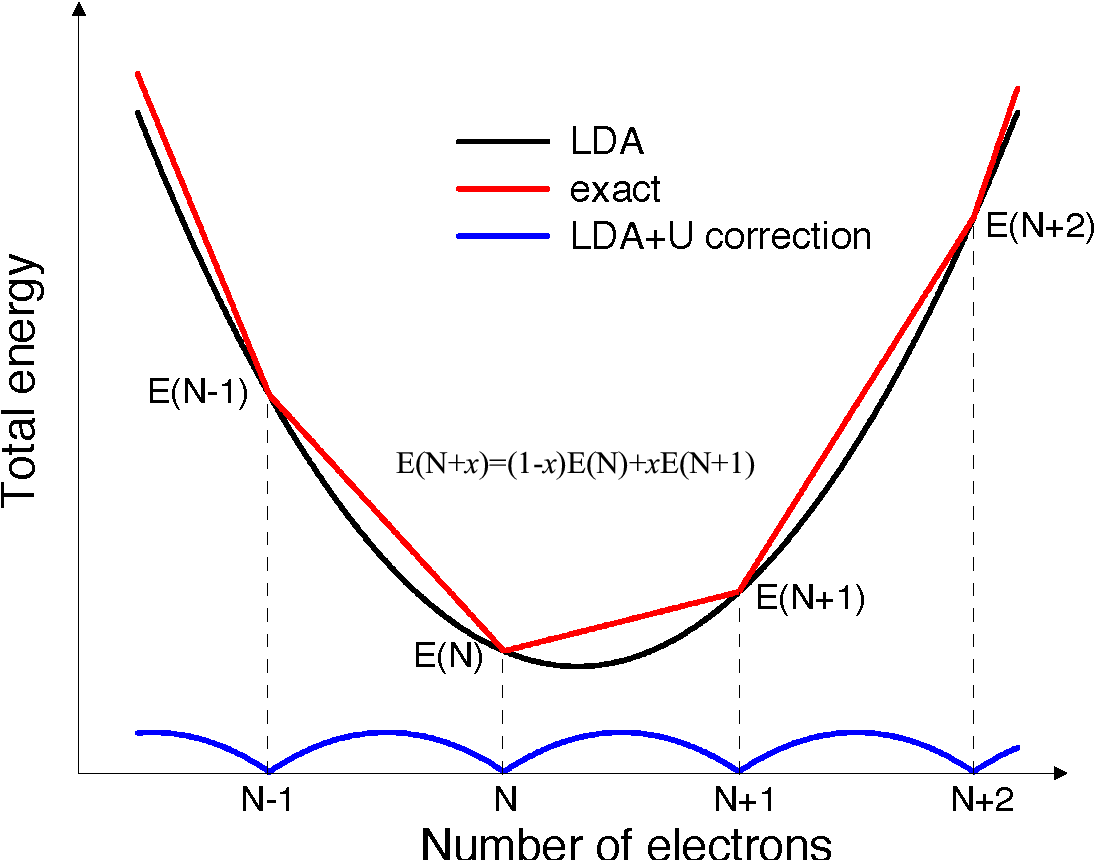
\includegraphics[height=2.4in,width=2.8in,viewport=0 0 1000 880,clip]{Koopmans-condition_LDA-U.png}
\caption{\small \textrm{The dependence of the total energy on the number of electron is a series of straight-line segments.}}%(与文献\cite{EPJB33-47_2003}图1对比)
\label{exact-DFT}
\end{figure}

Gunnarsson和Schonhammer\cite{PRL56-1968_1986}证明,单电子势的不连续对能带的带隙有很大的贡献。LDA泛函的另一个不足还在于,LDA计算得到的轨道能量(定义为能量$E$对轨道占据数$n_i$的导数,即$\varepsilon_i=\partial E/\partial n_i$),不满足\textrm{Koopmans}定理\cite{Physica1-104_1933},与实验或者严格计算得到的轨道能量差相去甚远。但是另一方面,LDA泛函得到的体系总能量一般与实验结果符合的较好。一个典型的例子就是\textrm{H}原子的计算,LDA计算的轨道能为$-0.54\,\mathrm{Ry}$(实际结果为$-1.0\,\mathrm{Ry}$),总能量($-0.976\,\mathrm{Ry}$)则非常接近$-1.0\,\mathrm{Ry}$\cite{PRB37-9919_1988}。文献\inlinecite{PRB44-943_1991}提出通过对LDA势加入轨道校正克服LDA方法的不足(称为LDA+$U$方法)。LDA+$U$方法与\textrm{Andersen}掺杂模型\cite{PR124-41_1961}思想相同,对局域的{\textit d}\,或{\textit f}\,电子,采用模型Hamiltonian方法考虑$d$-$d$或$f$-$f$间相互作用(定域Coulomb相互作用$U$),离域的{\textit s}\,和{\textit p}\,电子的运动用LDA近似描述。

%在文献\inlinecite{Herring}中,
\textrm{Herring}讨论了$U$值的物理意义:~含有$n$个3{\textit d}\,电子的原子中,如果定义两个原子间转移一个{\textit d}\,电子,即
$$2(d^n)\rightarrow d^{n+1}+d^{n-1}$$
能量的改变为$U$
$$U=E(d^{n+1})+E(d^{n-1})-2E(d^n)$$
在\textrm{DFT}框架下,\textrm{L(S)DA}是弱耦合的平均场(\textrm{mean-filed, MF})理论,对于{\textit d}\,电子数目发生变化的原子/离子体系,$d$-$d$电子间的相互作用可以表示为$E=UN(N-1)/2$\cite{PRB48-16929_1993},将总能量中扣除LDA的$d$-$d$电子相互作用,再加上局域的电子间相互作用,可有
\begin{equation}
  E=E_{LDA}-UN(N-1)/2+\frac12U\sum_{i\neq j}n_in_j
  \label{eq:solid-251}
\end{equation}
由式\eqref{eq:solid-251}对轨道占据数$n_i$求导得轨道能
\begin{equation}
  \varepsilon_i=\frac{\partial E}{\partial n_i}=E_{LDA}+U(\frac12-n_i)
  \label{eq:solid-252}
\end{equation}
\begin{figure}[h!]
\centering
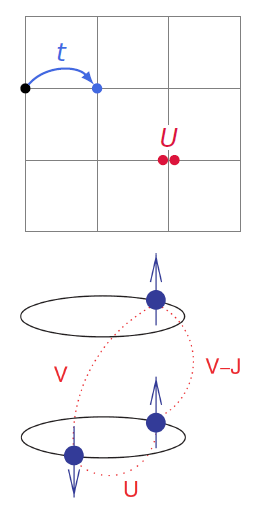
\includegraphics[height=1.35in,width=0.92in,viewport=1 1 240 375,clip]{LDA_U-1.png}
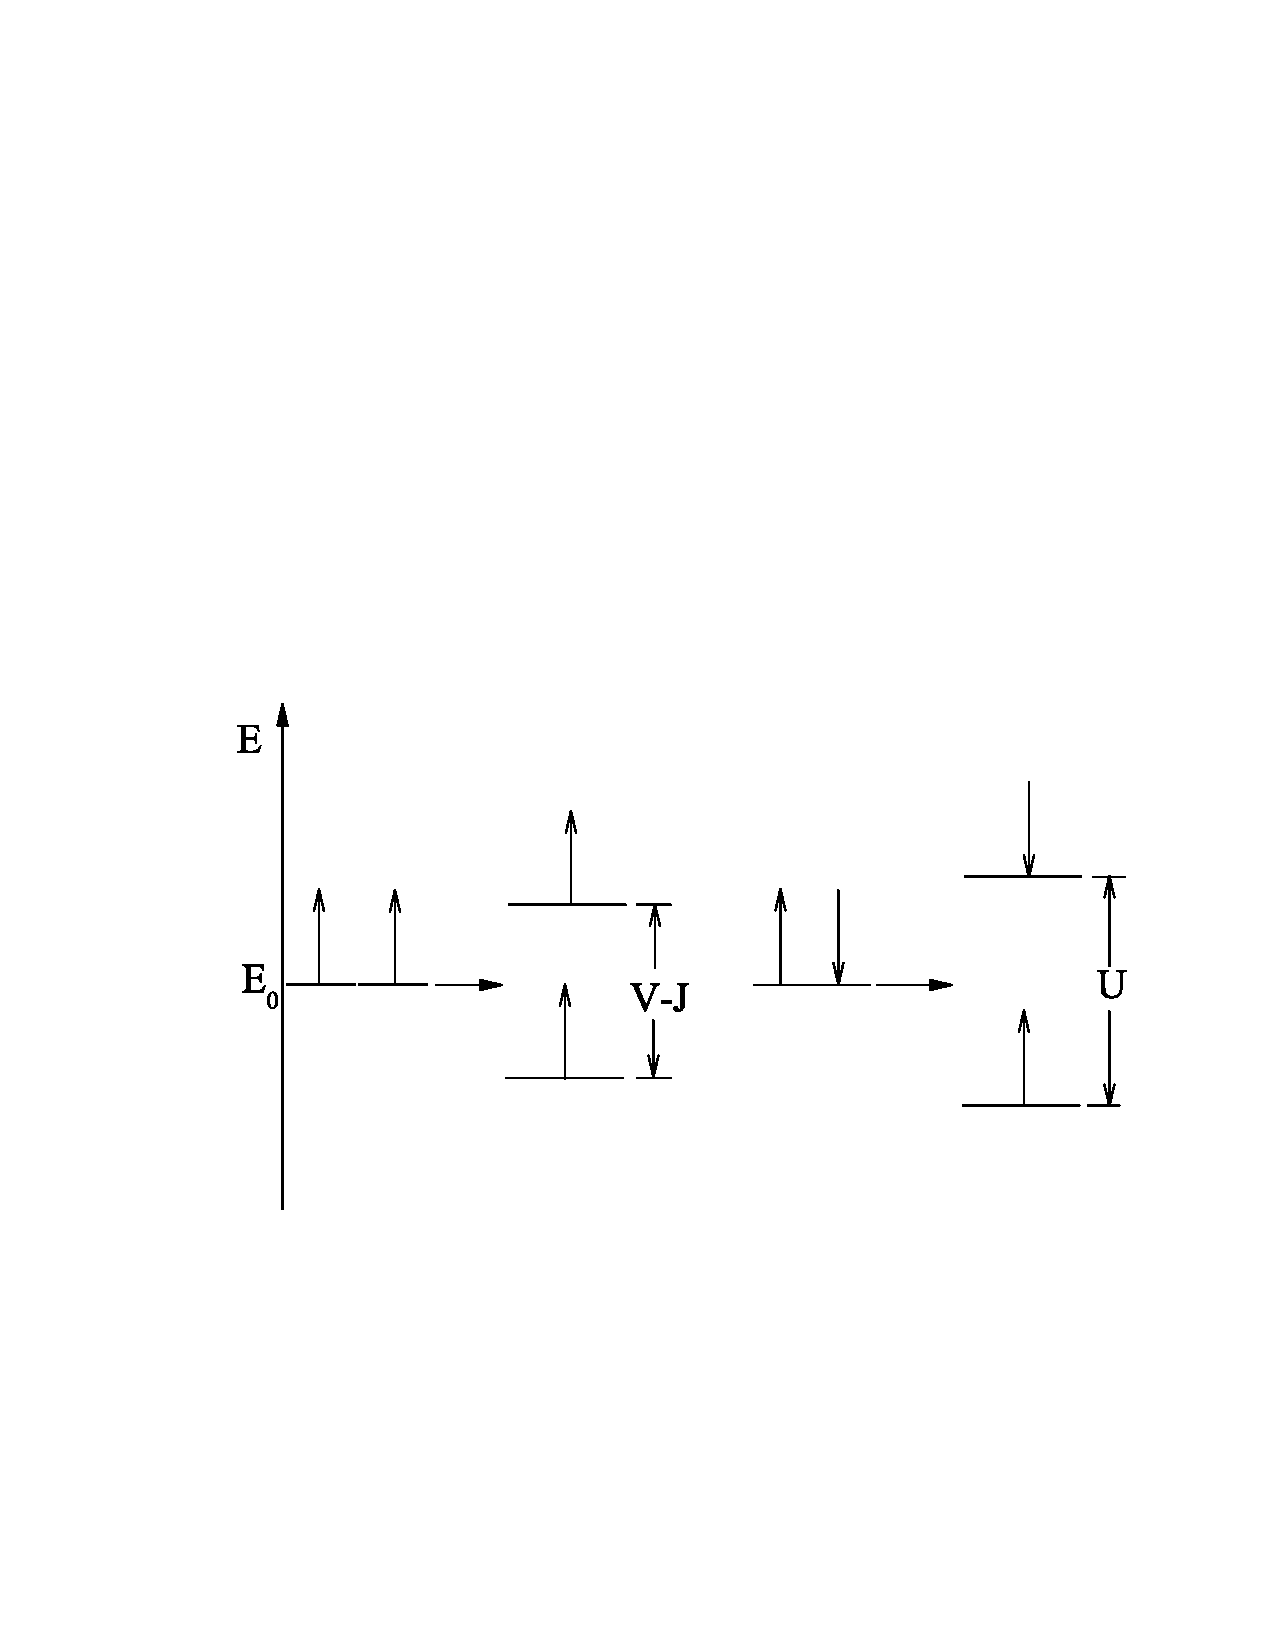
\includegraphics[height=1.35in,width=2.32in,viewport=110 210 545 455,clip]{LDA_U.pdf}
\caption{\small \textrm{The meaning of $U$, when the Coulomb-interaction of each electron is taken into account.}}%(与文献\cite{EPJB33-47_2003}图1对比)
\label{U_means}
\end{figure}
该式将占据态轨道($n_i$=1)和非占据态轨道($n_i$=0)的LDA轨道能分别移动-$U$/2和+$U$/2,由此得到的轨道相关势[$V_i(\vec r)=\delta E/\delta n_i(\vec r)$]为
\begin{equation}
  V_i(\vec r)=V_{LDA}(\vec r)+U(\frac12-n_i)
  \label{eq:solid-253}
\end{equation}
式\eqref{eq:solid-253}表明\textrm{LDA}+$U$,通过简单引入唯象参数$U$,保留了精确密度泛函理论的单电子势能所必需的不连续特征。图\ref{U_means}给出了参数$U$的物理含义示意:~$U$表示位于同一格点上电子间的排斥相互作用。

式\eqref{eq:solid-251}没有考虑相同自旋电子的交换作用。设自旋$\sigma$的{\textit d}-{\textit d}\,电子间交换参数为{\textit J}\,,则{\textit N}\,电子的LDA近似下{\textit d}-{\textit d}\,相互作用为$UN(N-1)/2-JN(N-2)/4$。

如果进一步考虑Coulomb势和交换势的非球形部分的贡献(与{\textit d}\,轨道的$m$和$m^{\prime}$相关部分),引入矩阵元$U_{mm^{\prime}}$和$J_{mm^{\prime}}$,有
\begin{equation}
  U_{mm^{\prime}}=\sum_ka_kF^k
  \label{eq:solid-210}
\end{equation}
\begin{equation}
  J_{mm^{\prime}}=\sum_kb_kJ^k
  \label{eq:solid-211}
\end{equation}
\begin{equation}
  a_k=\frac{4\pi}{2k+1}\sum_{q=-k}^k\langle lm|Y_{kq}|lm\rangle\langle lm|Y_{kq}^{\ast}|lm^{\prime}\rangle
  \label{eq:solid-212}
\end{equation}
\begin{equation}
  b_k=\frac{4\pi}{2k+1}\sum_{q=-k}^k|\langle lm|Y_{kq}|lm^{\prime}\rangle|^2
  \label{eq:solid-213}
\end{equation}
这里$F^k$是Slater积分,$\langle lm|Y_{kq}|lm^{\prime}\rangle$是三个球谐函数$Y_{lm}$的乘积的积分。

由此得到的总能量为
\begin{equation}
  \begin{split}
	  E=&E_{\mathrm{LDA}}-[UN(N-1)/2-JN(N-2)/4]\\
  &+\frac12\sum_{m,m^{\prime},\sigma}U_{mm^{\prime}}n_{m\sigma}n_{m^{\prime}\sigma}\\
  &+\frac12\sum_{m\neq m^{\prime},m^{\prime},\sigma}(U_{mm^{\prime}}-J_{mm^{\prime}})n_{m\sigma}n_{m^{\prime}\sigma}
  \end{split}
  \label{eq:solid-214}
\end{equation}
式\eqref{eq:solid-214}应占据数$n_{m\sigma}$求导,得到轨道相关的单电子势能
\begin{equation}
  \begin{split}
	  V_{m\sigma}(\vec r)=&V_{\mathrm{LDA}}(\vec r)+\sum_{m^{\prime}}(U_{mm^{\prime}}-U_{\mathrm{eff}})n_{m-\sigma}\\
	  &\sum_{m\neq m^{\prime}}(U_{mm^{\prime}}-J{mm^{\prime}}-U_{\mathrm{eff}})n_{m\sigma}+U_{eff}\left(\frac12-n_{m\sigma}\right)-\frac12J
  \end{split}
  \label{eq:solid-215}
\end{equation}
这里$U_{\mathrm{eff}}=U-J/2$。

为了计算矩阵元$U_{mm^{\prime}}$和$J_{mm^{\prime}}$,必须知道Slater积分$F^k$(对{\it d}\,电子是$F^0$,$F^2$和$F^4$)。文献\cite{PRB43-7570_1991}用超晶胞近似(supercell approximation)给出Coulomb参数$U$,和$F^0$相等,将矩阵元$U_{mm^{\prime}}$和$(U_{mm^{\prime}}-J_{mm^{\prime}})$对所有$mm^{\prime}$求平均,可以得到$U$和$(U-J)$,根据Clebsch-Gordan系数性质,有平均值为
\begin{equation}
  U=\frac1{(2l+1)^2}\sum_{mm^{\prime}}U_{mm^{\prime}}=F^0
  \label{eq:solid-216}
\end{equation}
\begin{equation}
  U-J=\frac1{2l(2l+1)}\sum_{mm^{\prime}}(U_{mm^{\prime}}-J_{mm^{\prime}})=F^0-(F^2+F^4)
  \label{eq:solid-217}
\end{equation}
\begin{equation}
  J=(F^2=F^4)/4
  \label{eq:solid-218}
\end{equation}
为了由$U$和$J$得到所有的Slater积分,只需要知道$F^4/F^2$\cite{PRB42-5459_1990}。

LDA+$U$方法最重要的特征是具备了单电子势的不连续性。计算表明LDA+$U$方法对含有定域强Coulomb相互作用的体系是可靠的\cite{PRB48-16929_1993,JPCS56-1521_1995,EPL36-551_1996}。无论对含有近芯层的局域4{\textit f}\,电子的稀土金属离子还是对过渡金属的氧化物(金属的3{\textit d}\,电子与氧原子2{\textit p}\,轨道有很强的相互作用)体系都有效。尽管LDA+$U$方法只是通过参数$U$唯象地考虑电子间的关联效应,并未突破平均场近似框架,因此不足以描述金属-绝缘体的\textrm{Mott}转变和具有强关联的金属。但对诸如FeSi和LaCaO$_3$这类化合物,LDA+$U$已经能够给出有关于金属-绝缘体转变的有用信息\cite{JPCM9-767_1997}。甚至对含有5{\textit f}\,电子的化合物的研究也取得一定的成功\cite{PRB54-R3706_1996}。

\subsection{电子激发与GW近似}
Landau的Fermi液体理论是研究群体激发和多体Fermi子体系物理性质的重要方法\cite{Landau}。Fermi液体的特征是准粒子分布$\varepsilon=\varepsilon(\vec k)$由体系总能量$E$对分布函数的变分,即
\begin{equation}
  \frac{\delta E}{\delta n(\vec k)}=\varepsilon(\vec k)
  \label{eq:solid-219}
\end{equation}
关联函数$f(\vec k,\vec k^{\prime})$由准粒子能量对整个$\vec k$空间粒子分布变分得到
\begin{equation}
  \frac{\delta\varepsilon(\vec k)}{\delta n(\vec k^{\prime})}=\frac{\delta^2E}{\delta n(\vec k)\delta n(\vec k^{\prime})}=f(\vec k,\vec k^{\prime})
  \label{eq:solid-220}
\end{equation}
考虑准粒子间相互作用,体系激发能记作
\begin{equation}
  W=\sum_{\vec k}\varepsilon(\vec k)\delta n(\vec k)+\frac12\sum_{\vec k}\sum_{\vec k^{\prime}}f(\vec k,\vec k^{\prime})\delta n(\vec k)\delta(\vec k^{\prime})
  \label{eq:solid-221}
\end{equation}

Green函数是研究Fermi液体的重要数学工具。对宏观体系,Green函数定义为\cite{Lifshitz}
\begin{equation}
	\tilde G(x,x^{\prime})=-\mathrm{i}\langle T\hat\Psi(x)\hat\Psi^{\ast}(x^{\prime})\rangle
  \label{eq:solid-222}
\end{equation}
这里$x$表示时间$t$和位置$\vec r$,$\langle\cdots\rangle$表示对体系基态求平均,$T$表示按时间先后乘积算符。$\hat\Psi$是Heisenberg算符,对式\eqref{eq:solid-222}进行Fourier变换,得到以$\vec r$,$E$为表象的Green函数$\tilde G(\vec r,\vec r^{\prime};E)$是Dyson方程\cite{Lifshitz}
\begin{equation}
	(\dfrac12\nabla^2+E)\tilde G(\vec r,\vec r^{\prime};E)-\int\mathrm{d}\vec r^{\prime\prime}\Sigma(\vec r,\vec r^{\prime\prime};E)\tilde G(\vec r^{\prime\prime},\vec r^{\prime};E)=\delta(\vec r-\vec r^{\prime})
  \label{eq:solid-223}
\end{equation}
的解。这里$\Sigma(\vec r,\vec r^{\prime};E)$是描述交换和相关效应的质量或自能算符,这是个与能量有关的非定域的非-Hermitian算符,考虑到粒子与体系中其他粒子的相互作用。晶体中的质量具有平移对称性,
\begin{equation}
  \Sigma(\vec r+\vec a,\vec r+\vec a;E)=\Sigma(\vec r,\vec r^{\prime};E),
  \label{eq:solid:224}
\end{equation}
这里$\vec a$是晶体平移格矢。

临近Green函数的极点,式\eqref{eq:solid-223}右面的$\delta$函数为0,所得积分-微分方程的本征值确定体系激发能谱\cite{Lifshitz,PR145-561_1966}
\begin{equation}
	-\delta^2\Phi_{\vec k}(\vec r,E)+\int\mathrm{d}\vec r^{\prime}\Sigma(\vec r,\vec r^{\prime};E)\Phi_{\vec k}(\vec r^{\prime},E)=\varepsilon_{\vec k}\Phi_{\vec k}(\vec r,E) 
  \label{eq:solid-225}
\end{equation}
这里函数$\Phi_{\vec k}(\vec r,E)$类似于周期场中的单电子Bloch波函数。对金属中的Fermi电子液体中用式\eqref{eq:solid-225}替代一般Schr\"odinger方程。与一般的Schr\"odinger方程不同,式\eqref{eq:solid-225}的能量本征值是复数,因为质量算符$\Sigma(\vec r,\vec r^{\prime};E)$是复数。

由式(\ref{eq:solid-223},\ref{eq:solid-225})得到Green函数
\begin{equation}
	\tilde G(\vec r,\vec r^{\prime};E)=\sum_{\vec k}\frac{\Phi_{\vec k}(\vec r,E)\Phi_{\vec k}^{\ast}(\vec r^{\prime},E)}{E-\varepsilon_{\vec k}(E)+\mathrm{i}0\mathrm{sgn}E}
  \label{eq:solid-226}
\end{equation}
$\varepsilon_{\vec k}(E)$是体系中加入一个粒子引起的能量改变。如果将单个准粒子改变引起得能量变化$\varepsilon_{\vec k}(E)$定义为式\eqref{eq:solid-219}中的准粒子能量,对临近Fermi面的态,函数$\tilde G(\vec r,\vec r^{\prime};E)$在$E=\varepsilon_{\vec k}(E)$有极值。因此Green函数极值确定了多Fermi子体系的元激发能谱。一般说,因为和其他粒子相互作用,准粒子能量为复数。复数能量使得体系激发态的寿命有限$(\tau\sim1/|\mathrm{Im}\varepsilon|)$\cite{Landau-Lifshitz}。能量宽度由$\mathrm{Im}\varepsilon$确定。

%临近Fermi能级,$\mathrm{Im}\varepsilon_{\vec k}(E)\rightarrow0$,相应的$\mathrm{Im}\Sigma\rightarrow0$,于是解方程\eqref{eq:solid-225}得到$\mathrm{Re}\varepsilon_{\vec k}(E)$和实数形式的$\Sigma(\vec r,\vec r^{\prime};E)$和$\epsilon_{\vec k}(E)$。

根据Hohenberg-Kohn定理,本征值$\Sigma(\vec r,\vec r^{\prime};E)$由体系基态确定,它也是电子密度的函数。Sham和Kohn建议可用局域电子密度近似表示$\Sigma(\vec r,\vec r^{\prime};E)$\cite{PR145-561_1966}:
\begin{equation}
  \Sigma(\vec r,\vec r^{\prime};E)=V_C(\vec r)\delta(\vec r-\vec r^{\prime})+\Sigma_0(\vec r-\vec r^{\prime};E-V_C(\vec r_0);\rho(\vec r_0))
  \label{eq:solid-227}
\end{equation}
这里$\Sigma_0$是密度为$\rho$的无相互作用电子气的本征能量,$V_C(\vec r_0)$是位于$\vec r_0=(\vec r+\vec r^{\prime})/2$的静电Coulomb势。此外式\eqref{eq:solid-227}已将能量$\Sigma$中的局域部分以Hartree势的形式分离出来,因此可以利用$\Sigma_0$的短程效应。

对本征函数$\Phi_{\vec k}$作近似
$$\Phi_{\vec k}(\vec r,E)=A(\vec k)\exp[\mathrm{i}\vec p(\vec r)\vec r]$$
并认为$A$和电子动量与$\vec r$无关,将式\eqref{eq:solid-225}称为类似Kohn-Sham方程的表达式\cite{JPC4-2064_1971},
\begin{equation}
  [-\dfrac12\nabla^2+V_C(\vec r)+\Sigma_{xc}(\rho(\vec r),E)]\Phi_{\vec k}(\vec r,E)=\varepsilon_{\vec k}(\vec r,E)
  \label{eq:solid-228}
\end{equation}
若$E=\mu$,$\Sigma_{xc}(\rho(\vec r),\mu)\equiv\mu_{xc}(\rho(\vec r))$我们因此得到符合局域密度近似的DFT方程,两者的交换-相关势$\mu_{xc}$是相同的。因此对于低激发能,可以使用近似$\Sigma_{xc}(\rho(\vec r),E)\simeq\mu_{xc}$,此结果对应于忽略准粒子间的相互作用,即Landau函数$f(\vec k,\vec k^{\prime})=0$。

因此基于DFT的能带计算,如果充分考虑交换-相关效应,可以计算多电子体系的元激发能量。注意,采用单电子近似,要求能带比较宽,即中心位于不同格点的波函数有较大的重叠,电子间相互作用不是很强。

Hedin和Lundqvist详细回顾了用Green函数技术解决电子相关的问题\cite{Hedin-Lundqvist}。在单粒子近似下的Green函数,准粒子与谱函数的峰联系在一起。如果峰足够尖锐,表明存在一个明确的准粒子能量,对一般的非均匀体系,准粒子能量和波函数可以通过解Dyson方程\eqref{eq:solid-225}求得。对于准粒子问题,核心问题是对自能算符$\Sigma(\vec r,\vec r^{\prime};E)$的足够好的近似。常用的方法是GW近似\cite{PR139-A796_1965},自能用屏蔽相互作用$W$计算到最低阶。
\begin{equation}
	\Sigma(\vec r,\vec r^{\prime};E)=\dfrac{\mathrm{i}}{2\pi}\int_{-\infty}^{\infty}\mathrm{d}E^{\prime}\tilde G(\vec r,\vec r^{\prime};E+E^{\prime})W(\vec r,\vec r^{\prime};E^{\prime})
  \label{eq:solid-229}
\end{equation}
Green函数$\tilde G$由准粒子的波函数和能量表示,屏蔽Coulomb作用$W$
\begin{equation}
	W(\vec r,\vec r^{\prime};E)=\frac1{\Omega}\int\mathrm{d}^3r^{\prime\prime}\varepsilon^{-1}(\vec r,\vec r^{\prime\prime};E)V(\vec r^{\prime\prime}-\vec r^{\prime})
  \label{eq:solid-230}
\end{equation}
这里$V$是未屏蔽的Coulomb势,$\varepsilon^{-1}$是介电函数矩阵的逆阵,
\begin{equation}
	\varepsilon^{-1}(\vec r,\vec r^{\prime};E)=\delta(\vec r-\vec r^{\prime})+\int\mathrm{d}^3r^{\prime\prime}V(\vec r^{\prime}-\vec r^{\prime\prime})P(\vec r^{\prime\prime},\vec r^{\prime};E)
  \label{eq:solid-231}
\end{equation}
这里$P$是完全响应函数,于是
\begin{equation}
  W(\vec r,\vec r^{\prime};E)=V(\vec r-\vec r^{\prime})+W_c(\vec r,\vec r^{\prime};E)
  \label{eq:solid-232}
\end{equation}
这里
\begin{equation}
	W_c(\vec r,\vec r;E)=\int\mathrm{d}^3r_1d^3r_2V(\vec r^{\prime}-\vec r_1)P(\vec r_1,\vec r_2;E)V(\vec r_2-\vec r^{\prime})
  \label{eq:solid-233}
\end{equation}
Green函数可以写成谱表示
\begin{equation}
	G(\vec r,\vec r^{\prime};E)=\int_{-\infty}^{\mu}\mathrm{d}E^{\prime}\frac{A(\vec r,\vec r^{\prime};E^{\prime})}{E-E^{\prime}-i\delta}+\int_{\mu}^{\infty}\mathrm{d}E^{\prime}\frac{A(\vec r,\vec r^{\prime};E^{\prime})}{E-E^{\prime}+i\delta}
  \label{eq:solid-234}
\end{equation}
这里$A(\vec r,\vec r^{\prime};E)=-\frac1{\pi}\mathrm{Im}G(\vec r,\vec r^{\prime};E)\mathrm{sgn}(E-\mu)$

实际计算中,取零阶Green函数,有
\begin{equation}
  A(\vec r,\vec r^{\prime};E)=\sum_{kn}\psi_{kn}(\vec r)\psi_{kn}^{\ast}(\vec r^{\prime})\delta(E-E_{kn})
  \label{eq:solid-235}
\end{equation}
于是自能可以写成
\begin{equation}
  \Sigma(\vec r,\vec r^{\prime};E)=\Sigma_x(\vec r,\vec r^{\prime})+\Sigma_c(\vec r,\vec r^{\prime};E)
  \label{eq:solid-236}
\end{equation}
这里$\Sigma_x$是净的交换势,
\begin{equation}
	\Sigma_x(\vec r,\vec r^{\prime})=-\sum_{kn}^{\mathrm{occ}}\psi_{kn}(\vec r)\psi_{kn}^{\ast}(\vec r^{\prime})V(\vec r-\vec r^{\prime})
  \label{eq:solid-254}
\end{equation}
$E_c$自能的相关部分,
\begin{equation}
  \begin{split}
	  \Sigma_c(\vec r,\vec r^{\prime};E)=&\sum_{kn}^{\mathrm{occ}}\psi_{kn}(\vec r)\psi_{kn}^{\ast}(\vec r^{\prime})W_c^-(\vec r,\vec r^{\prime};E-E_{kn})\\
	  &+\sum_{kn}^{\mathrm{occ}}\psi_{kn}(\vec r)\psi_{\vec r}^{\ast}(\vec r^{\prime})W_c^+(\vec r,\vec r^{\prime};E-E_{kn})
  \end{split}
  \label{eq:solid-237}
\end{equation}
其中$W_c^{\pm}(\vec r,\vec r^{\prime};E)=\dfrac{\mathrm{i}}{2\pi}\int_{-\infty}^{+\infty}\mathrm{d}E^{\prime}\frac{W_c(\vec r,\vec r^{\prime};E^{\prime})}{E+E^{\prime}\pm i\delta}$。于是$\Sigma(\vec r,\vec r^{\prime};E)$可以记作\cite{JPCM9-767_1997},
\begin{displaymath}
  \Sigma(\vec r,\vec r^{\prime};E)=-\sum_{kn}\psi_{kn}(\vec r)\psi_{kn}^{\ast}(\vec r^{\prime})W_0(\vec r,\vec r^{\prime};E-E_{kn})
\end{displaymath}
其中
\begin{displaymath}
  \begin{aligned}
    W_0(\vec r,\vec r^{\prime};E-E_{kn})\equiv&[V(\vec r-\vec r^{\prime})-W_c^-(\vec r,\vec r^{\prime};E-E_{kn})]\theta(\mu-E_{kn})\\
    &-W_c^+(\vec r,\vec r^{\prime};E-E_{kn})\theta(E_{kn}-\mu)
  \end{aligned}
\end{displaymath}
这样的GWA近似的自能与Hartree-Fock方法具有相同的形式,但是自能是能量的函数且因为包含相关作用,因此也依赖于未占据态。GWA可以看作是包含动态屏蔽Coulomb势$W_0$的推广Hartree-Fock方法,注意这里的$W_0$与动态屏蔽势$W$不同。

在各种能带计算方法中引入GW近似,包括赝势方法\cite{PRB34-5390_1986},LMTO-TB方法\cite{PRL74-3221_1995}。GWA校正主要应用于简单金属和过渡金属体系,但由于计算过程比较复杂所以目前还没有广泛应用到复杂体系的计算中。GWA校正的另一个问题是计算屏蔽相互作用所需的响应函数,要借助LDA得到的波函数和能带来计算得到\cite{JPCM9-767_1997}。但是这样的方法只适用于电子相关较小的体系(比如绝缘体或者半导体);对电子强相关体系,则需要采用比LDA近似更好的Hamiltonian,一般可以通过自洽迭代来计算自能\cite{PRL74-3221_1995}。

\subsection{LDA+$U$和GWA校正的关系$^\ast$}
尽管GWA是由多体微扰理论导出的最简单的自能近似,但是计算量已经很大。GWA和LDA+$U$可以分别看作包含依赖于频率和轨道屏蔽Coulomb作用的Hartree-Fock方法。至少对含有局域的{\textit d}\,或{\textit f}\,轨道的过渡金属和稀土金属离子,LDA+$U$可以看作是对GWA更粗略的近似\cite{JPCM9-767_1997}。

LDA+$U$是针对包含在离域态中的定域态轨道的自能校正,定域态的强Coulomb相关用参数$U$校正,而离域态可以用LDA很好的描述。为了确定LDA+$U$和GWA之间的关系,对态$\psi_d$,考虑GWA中自能的相关部分
\begin{equation}
  \begin{split}
    \langle\psi_d|\Sigma_c(E_d)|\psi_d\rangle=&\langle\psi_d\psi_d|W_c^-|\psi_d\psi_d\rangle\\
    &+\sum_{kn\neq d}^{\mathrm{occ}}\langle\psi_d\psi_{kn}|W_c^-(E_d-E_{kn})|\psi_{kn}\psi_d\rangle\\
    &+\sum_{kn}^{\mathrm{unocc}}\langle\psi_d\psi_{kn}|W_c^+(E_d-E_{kn})|\psi_{kn}\psi_d\rangle
  \end{split}
  \label{eq:solid-238}
\end{equation}
严格地说,自能应该是$\tilde E_d=E_d+$自能校正。如果$\psi_d$是局域的而且能量与其他态很好的分离,则式\eqref{eq:solid-238}第一项比剩下的其余项大得多,最后一项含未占据的$\psi_d$态,但因为这些项与占据态正交,因此这一项比第一项小得多。可作近似\cite{JPCM9-767_1997}
\begin{equation}
  \langle\psi_d|\Sigma_c(E_d)|\psi_d\rangle\approx\langle\psi_d\psi_d|W_c^-(0)|\psi_d\psi_d\rangle=-\frac12\langle\psi_d\psi_d|W_c(0)|\psi_d\psi_d\rangle
  \label{eq:solid-239}
\end{equation}
将屏蔽势关联部分写成谱函数表象,
\begin{equation}
	W_c(E)=\int_{-\infty}^0\mathrm{d}E^{\prime}\frac{B(E^{\prime})}{E-E^{\prime}-i\delta}+\int_0^{\infty}\mathrm{d}E^{\prime}\frac{B(E^{\prime})}{E-E^{\prime}+i\delta}
  \label{eq:solid-240}
\end{equation}
这里$B(E)=-\dfrac1{\pi}W_c(E)\mathrm{sgn}(E)$。
$W_c$是$E$的偶函数,因此$B(E)$是奇函数,因此$W_c^-(0)=-1/2W_c(0)$,类似的对未占据的{\textit d}\,态,有$+1/2\langle\psi_d\psi_d|W_c(0)|\psi_d\psi_d\rangle$,因此能量差为
\begin{equation}
  \begin{split}
	  \Delta&=E_2^{\mathrm{HF}}-E_1^{\mathrm{HF}}+\langle\psi_d\psi_d|W_c(0)|\psi_d\psi_d\rangle\\
    &=\langle\psi_d\psi_d|V|\psi_d\psi_d\rangle+\langle\psi_d\psi_d|W_c(0)|\psi_d\psi_d\rangle\\
    &=\langle\psi_d\psi_d|W(0)|\psi_d\psi_d\rangle
  \end{split}
  \label{eq:solid-241}
\end{equation}
这符合屏蔽Coulomb相互作用$\Delta=U\approx W(0)$。

上述近似中,局域态的GW自能为
\begin{equation}
  \Sigma(\vec r,\vec r^{\prime};E_d)=\Sigma_x(\vec r,\vec r^{\prime})+\sum_{kn=d}\psi(\vec r)\psi_{kn}^{\ast}(\vec r^{\prime})W_c^0(\vec r,\vec r^{\prime};E_d)
  \label{eq:solid-242}
\end{equation}
这里$$W_c^0(\vec r,\vec r^{\prime};E)=-\frac12W_c(\vec r,\vec r^{\prime};0)[\theta(\mu-E_d)-\theta(E_d-\mu)]$$
LDA的自能校正
\begin{equation}
  \Delta\Sigma(\vec r,\vec r^{\prime};E_d)=\Sigma(\vec r,\vec r^{\prime};E_d)-V_{xc}^{LDA}(\vec r)\delta(\vec r-\vec r^{\prime})
  \label{eq:solid-243}
\end{equation}
应该与LDA+$U$方法的$U$值相等。按照LDA+$U$思想,将空间分为定域部分$\phi_m$(一般是{\textit d}\,和{\textit f}\,态)和离域部分$\psi_{kn}$
$$\delta(\vec r-\vec r^{\prime})=\sum_m\phi_m(\vec r)\phi_m^{\ast}(\vec r^{\prime})+\sum_{kn}\psi_{kn}(\vec r)\psi_{kn}^{\ast}(\vec r^{\prime})$$
自能校正可以写成
\begin{equation}
  \begin{split}
    \Delta(\vec r,\vec r^{\prime};E_d)=&\sum_{mm^{\prime}}\phi_m(\vec r)\Delta\Sigma_{mm^{\prime}}(E_d)\phi_{m^{\prime}}^{\ast}(\vec r^{\prime})+\sum_{knn^{\prime}}\psi_{kn}(\vec r)\Delta\Sigma_{nn^{\prime}}(E_d)\psi_{kn}^{\ast}(\vec r^{\prime})\\
    &+\sum_{knm}\psi_{kn}(\vec r)\delta\Sigma_{nm}(\vec k,E_d)\phi_m^{\ast}(\vec r^{\prime})+\sum_{kmn}\phi_m(\vec r)\Delta\Sigma_{mn}(\vec k,E_d)\psi_{kn}^{\ast}(\vec r^{\prime})
  \end{split}
  \label{eq:solid-244}
\end{equation}
其中第一项是主要的,有近似
$$\Delta\Sigma(\vec r,\vec r;E_d)\approx\sum_{mm^{\prime}}\phi_m(\vec r)\Delta\Sigma_{mm^{\prime}}(E_d)\phi_{m^{\prime}}^{\ast}(\vec r^{\prime})$$
这里$$\Delta\Sigma_{mm^{\prime}}(E_d)=\langle\phi_m|\Sigma_x-V_{xc}|\phi_m\rangle+\sum_{m^{\prime}m^{\prime\prime}}\langle m,m^{\prime\prime}|W_c^0|m^{\prime\prime\prime},m^{\prime}\rangle n_{m^{\prime\prime},m^{\prime\prime\prime}}$$
这里$$n_{m^{\prime\prime},m^{\prime\prime\prime}}=\sum_{kn=d}\langle\phi_{m^{\prime\prime}}|\psi_{kn}\rangle\langle\psi_{kn}|\phi_{m^{\prime\prime\prime}}\rangle$$
注意到选择的$\phi_m$是原子内的局域轨道,剩下的自能很小,可以包含在单电子项中。

假设只有一个{\it d}\,轨道$\psi_{m\sigma}$的{\it d}\,离子,根据上述近似,局域态的GWA自能为
\begin{equation}
  \Sigma(\vec r,\vec r^{\prime};E_{m\sigma})=\Sigma_x(\vec r,\vec r^{\prime})+\sum_{m^{\prime}\omega^{\prime}}\psi_{m^{\prime}\omega^{\prime}}(\vec r)\psi_{m^{\prime}\sigma^{\prime}}^{\ast}(\vec r^{\prime})W_c^0(\vec r,\vec r^{\prime};E_{m\sigma})
  \label{eq:solid-245}
\end{equation}
这里$$W_c^0(\vec r,\vec r^{\prime};E_{m\sigma})=-\frac12W_c(\vec r,\vec r^{\prime};0)[\theta(\mu-E_{m\omega})-\theta(E_{m\sigma}-\mu)]$$
GWA中的电子-电子相互作用的总势能的矩阵元可以写成
\begin{equation}
  \begin{split}
	  \langle\psi_{m\sigma}&|V_{\mathrm{H}}+\Sigma_x+\Sigma_c|\psi_{m\sigma}\rangle\\
	  =&\sum_{m^{\prime}\sigma^{\prime}}^{\mathrm{occ}}\iint\mathrm{d}\vec rd\vec r^{\prime}\psi_{m\omega}^{\ast}(\vec r)\psi_{m\omega}(\vec r)V(\vec r-\vec r^{\prime})\psi_{m^{\prime}\sigma^{\prime}}^{\ast}(\vec r^{\prime})\psi_{m^{\prime}\sigma^{\prime}}(\vec r^{\prime})\\
	  &-\sum_{m^{\prime}}^{\mathrm{occ}}\iint\mathrm{d}\vec rd\vec r^{\prime}\psi_{m\omega}^{\ast}(\vec r)\psi_{m^{\prime}\omega^{\prime}}(\vec r)V(\vec r-\vec r^{\prime})\psi_{m\sigma}^{\ast}(\vec r^{\prime})\psi_{m^{\prime}\sigma^{\prime}}(\vec r^{\prime})\\
    &+\left(\frac12-n_{m\sigma}\right)\sum_{m^{\prime}}\iint\mathrm{d}\vec rd\vec r^{\prime}\psi_{m\omega}^{\ast}(\vec r)\psi_{m^{\prime}\omega^{\prime}}(\vec r)W_c(\vec r,\vec r^{\prime};0)\psi_{m\sigma}^{\ast}(\vec r^{\prime})\psi_{m^{\prime}\sigma^{\prime}}(\vec r^{\prime})
  \end{split}
  \label{eq:solid-246}
\end{equation}
这里$n_{m\sigma}$是$m\sigma$轨道占据状态,如$\mu-E_{m\sigma}>0$则$n_{m\sigma}=1$;$\mu-E_{m\sigma}<0$,有$n_{m\sigma}=0$。上述矩阵元可以写成
$$V_{m\sigma}^{\mathrm{GWA}}=\sum_{m^{\prime}\sigma^{\prime}}U_{mm^{\prime}}^0n_{m^{\prime}\sigma^{\prime}}-U_{mm}^0n_{m\sigma}-\sum_{m^{\prime}\neq m}J_{mm^{\prime}}n_{m^{\prime}\sigma}+\left(\frac12-n_{m\sigma}\right)\sum_{m^{\prime}}W_{mm^{\prime}}$$
这里$U_{mm^{\prime}}^0$是未屏蔽的Coulomb相互作用矩阵元。$J_{mm^{\prime}}$是交换矩阵,$W_{mm^{\prime}}$是交换势$W_c(\vec r,\vec r^{\prime};0)$矩阵元。将屏蔽参数定义为$W=-\sum\limits_{m^{\prime}}W_{mm^{\prime}}$,最终GWA的势能矩阵元表达式为\cite{JPCM9-767_1997}
\begin{equation}
	V_{m\sigma}^{\mathrm{GWA}}=\sum_{m^{\prime}\sigma^{\prime}}U_{mm^{\prime}}^0n_{m^{\prime}\sigma^{\prime}}-(U_{mm}^0-W)n_{m\sigma}-\sum_{m^{\prime}\neq m}J_{mm^{\prime}}n_{m^{\prime}\sigma}-\frac12W
  \label{eq:solid-247}
\end{equation}
为了将LDA的校正写成GWA形式,必须将LSDA的势能矩阵元写成上述相似的形式,因为LSDA并非由轨道-轨道相互作用导出,而由类似于均匀电子气的处理方式,用与Coulomb相互作用能有关的电荷密度计算得到的与轨道无关的有效局域势,无法严格处理。{\textit d}\,电子的相互作用能作为总的{\textit d}\,电子数$N$的函数,$E_{\mathrm{LSDA}}[\rho(\vec r)]=E_{\mathrm{LSDA}}[N|\psi_{m\sigma}(\vec r)|^2]$。已知LSDA中单电子本征能不是很准确,但是总能量比较准确,于是假设Hartree-Fock计算是好的近似
\begin{equation}
  \begin{split}
	  E_{\mathrm{LSDA}}[\rho_{\sigma}(\vec r)]&=E_{\mathrm{LSDA}}[N_{\sigma}|\psi_{m\sigma}(\vec r)|^2]\\
   &=\frac12F^0N(N-1)-\frac14JN(N-2)\frac14J(N_{\uparrow}-N_{\downarrow})^2
 \end{split}
  \label{eq:solid-248}
\end{equation}
这里$F^0$是第一Slater积分,$J$是交换能参数,$N_{\sigma}=\sum\nolimits_mn_{m\sigma}$,$N=N_{\uparrow}+N_{\downarrow}$

LSDA的电子相互作用势能是总能量对电荷密度$\rho(\vec r)$的变分导数,相互作用能作为总的{\it d}\,电子总数$N_{\sigma}$的变分导数为:
\begin{equation}
  \begin{split}
	  \frac{\partial E_{\mathrm{LSDA}}[N_{\sigma}|\psi_{m\sigma}(\vec r)|^2]}{\partial N_{\sigma}}&=\int\mathrm{d}\vec r\frac{\delta E_{\mathrm{LSDA}}[\rho(\vec r)]}{\delta\rho_{\sigma}(\vec r)}\frac{\partial\rho_{\sigma}(\vec r)}{\partial N_{\sigma}}\\
	  &=\int\mathrm{d}\vec rV_{\mathrm{LSDA}}^{\sigma}(\rho(\vec r))|\psi_{m\sigma}(\vec r)|^2\\
    &=F^0N-\frac12(F^0-J)-JN_{\sigma}
  \end{split}
  \label{eq:solid-257}
\end{equation}
由此可有LSDA的势能矩阵元为$V_{m\sigma}^{\mathrm{LSDA}}=F^0N-\frac12(F^0-J)-JN_{\sigma}$。
GWA对LSDA的势能校正为\cite{JPCM9-767_1997}
\begin{equation}
  \begin{split}
	  \delta V_{m\sigma}=&V_{m\sigma}^{\mathrm{GWA}}-V_{m\sigma}^{\mathrm{LSDA}}\\
    =&\sum_{m^{\prime}\sigma^{\prime}}U_{mm^{\prime}}^0n_{m^{\prime}\sigma^{\prime}}-(U_{mm}^0-W)n_{m\sigma}-\sum_{m^{\prime}\neq m}j_{mm^{\prime}}n_{m^{\prime}\sigma}-\frac12W\\
    &-F^0\sum_{m^{\prime}\sigma^{\prime}}n_{m^{\prime}\sigma^{\prime}}+J\sum_mn_{m\sigma}+\frac12(F^0-J)\\
    =&\sum_{m^{\prime}\sigma^{\prime}}(U_{mm^{\prime}}^0-F^0)n_{m^{\prime}\sigma^{\prime}}-(U_{mm}^0-W)n_{m\sigma}-\sum_{m^{\prime}\neq m}j_{mm^{\prime}}n_{m^{\prime}\sigma}\\
    &-\frac12W+J\sum_mn_{n\sigma}+\frac12(F^0-J)
  \end{split}
  \label{eq:solid-249}
\end{equation}
差值$U_{mm^{\prime}}^0-F^0$与Slater积分$F^0$无关(只与Slater积分$F^k$且$k\neq0$有关),而且有$U_{mm^{\prime}}^0-F^0=U_{mm^{\prime}}-U$,这里$U=F^0-W$是屏蔽Coulomb参数,$U_{mm^{\prime}}$是屏蔽Coulomb矩阵元。
\begin{equation}
  \begin{split}
	  \delta V_{m\sigma}=&V_{m\sigma}^{\mathrm{GWA}}-V_{m\sigma}^{\mathrm{LSDA}}\\
    =&\sum_{m^{\prime}}U_{mm^{\prime}}n_{m^{\prime}-\sigma}+\sum_{m^{\prime}\neq m}(U_{mm^{\prime}}-J_{mm^{\prime}})n_{m^{\prime}\sigma}\\
    &-U(N-\frac12)+J(N_{\sigma}-\frac12)
  \end{split}
  \label{eq:solid-250}
\end{equation}
如果占据矩阵是对角化的,式\eqref{eq:solid-250}等价于LDA+$U$势校正\eqref{eq:solid-215}。GWA和LDA+$U$的本质差别在于计算屏蔽Coulomb势参数$U$,在LDA+$U$中,$U$是通过构造LSDA超晶胞计算的,在GWA中则是通过计算响应函数得到的。
%\newpage
%\bibliographystyle{mythesis}
%%  \phantomsection\addcontentsline{toc}{section}{bibliography}
%  {\small\bibliography{bib/Myref}}
%%  \nocite{*}
